\documentclass[lettersize,journal]{IEEEtran}
\usepackage{tabularx}
%\usepackage{subcaption}
%\usepackage{subfig}
\usepackage{floatrow}
\usepackage{colortbl}
\usepackage{amsmath,amsfonts}
\usepackage{algorithmic}
\usepackage{algorithm}
\usepackage{array}
\usepackage[caption=false,font=normalsize,labelfont=sf,textfont=sf]{subfig}
\usepackage{textcomp}
\usepackage{stfloats}
\usepackage{pgfplots}
\pgfplotsset{compat=1.18}
%\usepackage[breaklinks]{breakurl}
\usepackage{url}
\usepackage{verbatim}
\usepackage{graphicx}
\setlength{\marginparwidth}{2cm}
\usepackage{todonotes}
\usepackage{tikz}
\usepackage{pgf-pie}
\usepackage{xcolor}
\usepackage[noadjust]{cite}
\hyphenation{op-tical net-works semi-conduc-tor IEEE-Xplore}
% updated with editorial comments 8/9/2021
\definecolor{cor_tabela}{cmyk}{0.2706, 0.102, 0.102, 0.075}
\definecolor{cor_destaque}{cmyk}{0.4, 0.15, 0.15, 0.15}

\begin{document}

\title{A Systematic Mapping of Autonomous Vehicle Prototypes: Trends and Opportunities}

\author{Ericson Silva,
        Felipe Soares,
        Wenderson Souza,
        and~Henrique Freitas,~\IEEEmembership{Member,~IEEE},% <-this % stops a space

\thanks{The authors are with the Department of Computer Science, Pontificia Universidade Católica de Minas Gerais, Belo Horizonte,  30535-901, Brazil (e-mail: marquiere@unifei.edu.br; falsoares@sga.pucminas.br; juniowenderson@gmail.com; cota@pucminas.br)}% <-this % stops a space
\thanks{Manuscript received October X, 2023; revised Month Day, Year.}}

% The paper headers
% \markboth{Journal of \LaTeX\ Class Files,~Vol.~14, No.~8, August~2021}%
% {Shell \MakeLowercase{\textit{et al.}}: A Sample Article Using IEEEtran.cls for IEEE Journals}

\markboth{IEEE Transactions on Intelligent Vehicles}%
{Silva \MakeLowercase{\textit{et al.}}: A Systematic Mapping of Autonomous Vehicle Prototypes: Trends and Opportunities}

% \IEEEpubid{0000--0000/00\$00.00~\copyright~2021 IEEE}
% Remember, if you use this you must call \IEEEpubidadjcol in the second
% column for its text to clear the IEEEpubid mark.

\maketitle

\begin{abstract}
Autonomous driving vehicles (ADVs) are the next significant evolution in transportation systems. Using machine learning techniques supported by strong processing units and sensors, the driver would be removed and the vehicle would drive itself, bringing countless advantages to the commuting system. There are too many players developing their own ADV prototypes all over the world. For this reason, this paper aims to use a systematic mapping study (SMS) to identify trends and patterns in ADV development. From a set of academic databases, a total of 68 papers were selected from a total of 548 after applying inclusion and exclusion criteria and snowballing techniques. The results showed the technical characteristics of the platform required to develop real-size and mini ADV prototypes. In addition, the paper explains the detailed software and hardware architectures and their main aspects and requirements. Finally, the paper discusses the necessary set of sensors which are required and their characteristics and main suppliers. It was possible to map the publications distribution based on venues, year, authors' affiliation, and most prolific countries. This work can guide researchers to design their ADV prototype or identify development bottlenecks that could lead to narrow research and innovation possibilities in autonomous driving vehicle development.

\end{abstract}

\begin{IEEEkeywords}
Autonomous Driving Vehicle, Self-Driving Vehicle, Autonomous Vehicle Prototypes, Systematic Mapping Study
\end{IEEEkeywords}

\section{Introduction}
\IEEEPARstart{T}{he} Autonomous Driving  Vehicle (ADV) is almost a reality, and it is considered the next significant innovation in the upcoming years \cite{Rosenzweig2015}. All the major automakers and research groups spread all over the world are researching this technology and are showing their results in competitions or published papers \cite{Rosenzweig2015,Behere2015,Kato2015,Broggi2015}. As forecasted \cite{Liu2017c}, we entered 2020 in a mixed-mode era where ADV and traditional vehicles coexist. In 2040, traditional vehicles might even be forbidden to be on the streets, with only autonomous vehicles.

The adoption of autonomous vehicles are growing. In 2018, the Baidu auto company Apollo started mass production and deployed its autonomous minibus to run in geo-fenced areas in China \cite{Apollo}. In addition, the Chinese company Pony.ai has begun its self-driving taxi service in the city of Irvine \cite{Pony}. Google Company Waymo is offering a free ride in its upcoming autonomous taxi service in Phoenix East Valley  \cite{waymo} both in the USA. PerceptIn \cite{PerceptIn} is offering a low cost and low speed electrical autonomous vehicles to use in geo-fenced areas for travel distances between 1 to 5 miles in some countries in the world. Furthermore, during the COVID-19 outbreak in 2020, Cruise, a General Motors autonomous vehicles branch, made over fifty thousand contactless deliveries of meals in San Francisco to vulnerable communities using its self-driving fleet \cite{Cruise}. 

The Society of Automotive Engineers \cite{SAE} has defined levels of automation in vehicles. The ultimate goal is to reach level five, a fully automated vehicle. That means that the vehicle would have full capability to understand the environment in all weather conditions and navigate from one destination to another without any human intervention \cite{Lin2018}. It will cause a revolution in the transportation system, and the benefits are enormous. 

A massive reduction of problems like traffic congestion, accidents, parking space, vehicle insurance, and increased car sharing possibilities are some advantages expected from implementing the ADV \cite{Bimbraw2015} that aims to give comfortable, efficient, and safe driving for all. Fausten et al. \cite{Fausten2015} and Bartl and Rosenzweig \cite{Rosenzweig2015} put the advantages in numbers stating that we could achieve 80\% improvement in traffic throughput, 23\% to 39\% of fuel economy, an increase of 50\% of senior citizens mobility, 90\% reduction of traffic accidents and reduction to only 15\% of the actual car fleet.

Multiple technologies are combined in the ADV, making it a complex distributed information technology system \cite{Traub2017}. The final product will be a combination of results in research and development in several fields \cite{Kato2015}. Hardware, sensors, software stack, computing units, and \textcolor{black}{network protocols} capable of matching the requirements of the upcoming ADV are a topic of discussion among researchers \cite{Liu2017,Munir2018,Jo2015,Ziegler2014,Kato2015,tropea2021}.

However, there are too many results, and with the technology's rapid evolution, many hardware and software studied could be already outdated. 

The best way to understand what is working in this field of research is to look into the prototypes developed by car manufacturers and the research community. Even with the improvement of ADV simulation tools such as the digital twin simulation based \cite{yu2022}, that reduce the hours of road testing necessary to validate autonomous vehicles developments, the prototype will always be required. 



However, the car manufacturers' prototype details are often unavailable due to the fierce competition between the companies to become the first to deliver the ADV to the market. As a result, companies like Google, Uber, and Tesla hide their development details from the public. On the other hand, some companies make development details accessible. For example Nvidia offers a range of products to developers \cite{Nvidia} and Apollo \cite{Apollo} that goes even further, making its ADV code available on GitHub for anyone to use. These companies seek to be responsible for providing the necessary technology to developers to make autonomous vehicles.

\textcolor{black}{It is essential to understand how prototypes are being developed. Looking into the literature, it is possible to compare how the authors and manufacturers deal with the ADV prototype to find the best path for a suitable platform to test and develop autonomous driving systems. The first big choice is whether we go big or small. Is the real-size car necessary to develop autonomous vehicles, or could a miniature be used that would produce the same results as the real-size vehicle?}

\textcolor{black}{Going further, a discussion of what characteristics a vehicle has is critical. Every prototype has a different shape regarding sensors, hardware, and software. Finding a pattern in this development heterogeneity facilitates the research community toward a common goal. With many other issues to be addressed, the development of the ADV prototype has to be a stage to be quickly overcome so that the community can advance towards a myriad of other issues that surround the real deployment of intelligent transportation systems where the ADV is part of the whole scenario and not everything.}.


This paper focuses on mapping the recent and relevant published papers of ADV prototypes on real and diminished scales that had their development details disclosed. This mapping also includes the companies' development platforms for the research community. A Systematic Mapping Study (SMS) is used to structure a research area and provide an extensive overview \cite{keele2007guidelines}. The results of this study generate a report and visual data that shape the research field based on the research questions defined by Petersen et al. \cite{petersen2015guidelines}. 

\textcolor{black}{We intend to search for specific details regarding hardware, software, and sensors by cross-relating the information collected in the mapped prototypes. Specifically, we want to find the set of sensors necessary to build an ADV and design and architect hardware and software based on the intersection of features repeated in the prototypes mapped in the study. This mapping study aims to find prototypes that attempt to work without human interference, i.e., levels 4 and 5 of automation.}

\textcolor{black} {Hence, our goal is to find trends in ADV development by analyzing available prototypes that could lead to common choices for autonomous vehicle hardware, software, and sensors, as mentioned previously. Furthermore, it could guide and accelerate other researchers and developers to build prototypes or research platforms. In this work, aspects related to, e.g., vehicle networking, security, and simulation that do not deliver a prototype will not be addressed, as the aim is the development of the ego vehicle as a first step for those who want to start researching in this field with actual hardware and not simulation. Thus, our main contribution is the following:}

 \begin{itemize}
     \item A systematic mapping of recent papers in modern ADV prototypes development showing trends, technologies, and research opportunities.
 \end{itemize}
 
 The remainder of this paper is organized as follows: Section II presents the related work, Section III describes the research method, Section IV shows and analyzes the results, Section V presents threats to validity, Section VI discusses open research issues, and Section VII concludes this paper.


\section{{Related Work}\label{background}}


\textcolor{black} {
Systematic Mapping Study (SMS) plays an important role by offering a comprehensive overview of a particular field or area of interest. It enables researchers to identify the scope and depth of research within a specific domain, uncover patterns, trends, and gaps in the literature, and determine the concentration of studies across various categories, such as methodology, research focus, and results. } Our study found papers \cite{Bimbraw2015,Rosenzweig2015} that discuss the evolution of ADV research over the years and one paper \cite{Hussain2019} that did a systematic review of the existing situation of the research publications and results in all aspects regarding the ADV. This last paper lists other review papers discussing regulations, localization, and mapping. However, none focused on the aspects of hardware and software most applied in the autonomous vehicles being developed and tested.

In addition to the listed papers in Hussain and Zeadally \cite{Hussain2019} extensive survey, we located some papers that would map, review or survey specific aspects of the ADV, such as software techniques \cite{Bresson2017,Paden2016,Bevly2016}, machine learning application \cite{Mozaffari2020,Aradi2020}, external aspects related to the ADV \cite{Barnett2020,ElKhatib2020,Brito2017}, \textcolor{black}{vehicle-to-everything (V2X) networking \cite{hakak2023,ahangar2021,wu2023}, and cybersecurity related to autonomous vehicles \cite{PHAM2021, KIM2021, LIMBASIYA2022, sun2022} }. However, these topics differ from the ones covered in our mapping study.

\vspace{1em}

\subsubsection {\textcolor{black}{\textbf{History and Expectations}}}

\leavevmode\vspace{0.1\baselineskip}%

\textcolor{black}{The next two reviews papers explore the history of ADV development}. Bimbraw k. \cite{Bimbraw2015} traces a historical line from the first attempts to create an autonomous vehicle in 1926 to what is happening until 2015, and the trends for the future, dividing the paper into three relevant sections, as follows: historical antecedents, current progress, and prospective predictions. The author discussed what has changed in the past and what would change in the future in the population's regulations, laws, and daily life. Although the paper details the sensors applied during the ADV evolution, it does not mention the software and hardware used or their evolution in the vehicles. 

Bartl and Rosenzweig \cite{Rosenzweig2015} also bring a historical view focusing on the automotive evolution in the past 65 years with highlighting milestones in the progression of the technology. Furthermore, it tries to understand the research development in autonomous driving in the last years and to find the research gap by analyzing 399 academic publications from 1989 to 2015. The focus was to show publications over time, journal count, citation analysis, and most publication topics covered. Even though, at some point, the paper states that technology development will not soon be the main concern of researchers and developers, the authors found that 91,2\% of the papers published focus on technology development. Therefore, technology development is still, up to now, the main topic of interest in ADV.

Silva et al. \cite{SILVA2022154615} systematically reviewed the scientific literature on the environmental impacts of autonomous vehicles. The results reveal the benefits of autonomous vehicles due to improved techniques, new design possibilities, and better traffic flow. Finally, Li et al. \cite{LI2021101686} provides a systematic review of 80 studies. They researched future autonomous vehicles in urban mobility and logistics using an agent-based model, focusing on publications in urban areas and highlighting possibilities for future urban mobility and logistics integration.


\vspace{1em}

\subsubsection {\textcolor{black}{\textbf{Technological Review}}}

\leavevmode\vspace{0.1\baselineskip}%


S. Liu et al. \cite{Liu2017} comprehensively reviewed the computing systems needed for ADV, showing what has been done so far. Instead of mapping the application of technologies or researching trends, their focus was primarily on identifying and addressing the bottlenecks in technology development. Their book \cite{liu2020} condensed all the information regarding the ADV to lead researchers to build their own prototype. The emphases was on keeping the cost of the development as low as possible by using as an example its developed ADV that had been deployed in real life applications.

Hussein and Zeadaly \cite{Hussain2019} bring an extensive review of autonomous vehicles, emphasizing the communication aspects and discussing the state-of-the-art research results. Furthermore, the authors discuss the technological and non-technological challenges for ADV deployment as humanity's next source of transportation. However, their work still needs to give information about the software and hardware of the ADV in the available prototypes and deployed vehicles. It extensively reviews significant players and their challenges in building an ADV. However, it tends to emphasize the American companies' results and does not fully examine the attempts of significant players worldwide, such as the Chinese companies Pony.IA \cite{Pony} and Apollo \cite{Apollo}, or the Japanese ZMP \cite{ZMP} that had promising results in the ADV development.


S. Liu et al. \cite{Liu2019} reviewed all technologies applied in the ADV, ranging from sensors, computing units, runtime systems, middlewares, algorithms used to process the ADV common tasks, and vehicle-to-vehicle-to-anything networks. They dedicated a section to present the innovations in each vehicle subsystem, architecture, and network and show the challenges that the technology would encounter, focusing on the security features which are a new concern among researchers. That paper shows many authors' attempts to solve each topic's specific ADV challenge or problem. However, it does not show the most applied technology in each aspect of the ADV nor map the application of the technology in the research community.


Lopes et al. \cite{10.1145/3466933.3466990} followed the method of systematic literature to review 69 primary studies and to understand the technological limitations and impacts of using autonomous cars about feasibility, adaptation, traffic legislation, perceived benefits, people´s relation to cars and impacts on urban mobility. Khan et al. \cite{10.1145/3485767} discussed organizational issues that need to be addressed to achieve the highest level of automation in autonomous vehicles: sensors, communication, mobile edge computing, machine learning, data analytics, and distributed learning. 

\vspace{1em}

\subsubsection {\textcolor{black}{\textbf{Sensing and Perception Review}}}

\leavevmode\vspace{0.1\baselineskip}%

Some reviews were done specifically in the realm of sensing and perception systems of the ADV \cite{KHATAB202136,van2018,rosique2019}.
Khatab et al. \cite{KHATAB202136} presented operations and challenges of autonomous driving and reviewed state of the art in technologies, focusing on the sensory systems and algorithms. Van Brummelen et al. \cite{van2018} goes beyond the sensory systems, reviewing the entire perception system of the ADV including mapping and planning. It historically shows the problems solved by researchers and the most recent advances in the perception field for autonomous vehicles. Rosique at al. \cite{rosique2019} also did similar work by doing a systematic review of the ADV perception system. In addition, they also systematically reviewed many simulators for self-driving systems and its performances by comparing them the real life hardware.

\vspace{1em}

\subsubsection {\textcolor{black}{\textbf{Communication and Security Review}}}

\leavevmode\vspace{0.1\baselineskip}%

 \textcolor{black}{A critical component is the implementation of robust vehicle communication technologies. Key studies have reviewed the developments of communication technologies and their implications. Ahangar et al. \cite{ahangar2021} focus on enabling communication technologies that go from traditional short-range systems such as Bluetooth to more sophisticated networks such as cellular V2X (C-V2X) and 5G advances, underscoring their pivotal role in the safety and functionality of an autonomous vehicle. Meanwhile, hakak et al. \cite{hakak2023} broaden the scope to examine the comprehensive challenges and future trajectories of V2X communications, addressing interoperability issues and the critical need for robust infrastructure, especially in deploying 5G networks. On the other hand, Wu et al. \cite{wu2023} dive into the specific implications of V2X technologies within intelligent transportation systems (ITS), highlighting the essential nature of these communications to achieve the full potential of autonomous driving while highlighting the need for standardized security measures.}
 
  \textcolor{black}{The advent of implementing communication networks in autonomous vehicles, evolving them from an ego vehicle to a connected and autonomous vehicle, brought many security issues, which became a hot topic among the research community. Sun et al. \cite{sun2022} provide a comprehensive survey, categorizing cybersecurity risks into in-vehicle network attacks and external communications vulnerabilities, and present defense mechanisms critical for safeguarding ADV against potential cyber-attacks. Limbasiya et al. \cite{LIMBASIYA2022} explore the challenges introduced by adopting 6G technologies in ADV, highlighting the need for resilient malware code frameworks and advanced control-oriented defense strategies tailored to the unique requirements of a 6G-enabled infrastructure. Further compounding these challenges, Moubayed et al. \cite{moubayed2022} discuss the critical role of AI in enhancing the cyber security posture of ADV, focusing on AI-driven predictive analytics and anomaly detection systems designed to identify and neutralize cyber threats preemptively. Alazab et al. \cite{alazab2023} emphasize the importance of a holistic cybersecurity framework that includes technical solutions and regulatory standards to address the various cyber risks facing ADV. This includes advocating for continuous innovation in cyber-defense technologies and establishing rigorous cybersecurity standards and protocols.}

\vspace{1em}

\subsubsection {\textcolor{black}{\textbf{Overview}}}

\leavevmode\vspace{0.1\baselineskip}%
 
Table \ref{table:relatedWorks} compares related work and our proposed work in the context of Autonomous Driving Vehicles (ADVs). In summary, our proposal maps the recent papers on modern ADV prototype development, showing technologies, trends, and research opportunities. Furthermore, it brings detailed technical information on hardware, software, and sensors. Finally, the papers are organized to present the main publication aspects in this field of study.

\begin{table}[!ht]
  \centering  
  \captionsetup{
    format=hang, % Add this line to create hanging indent for the caption
    justification=raggedright,
    singlelinecheck=false,
    skip=9pt, % Adjust the distance between caption and table
  }
  \caption{\MakeUppercase{RELATED WORK OVERVIEW}}
  \label{table:relatedWorks}
  \def\arraystretch{1.09}
  \begin{tabularx}{\textwidth}{>{\centering\arraybackslash}m{1.7cm}>{\centering\arraybackslash}m{1.7cm}X}
    \arrayrulecolor{white}
    \rowcolor{white}
    \textbf{Works} & \textbf{Year} & \textbf{Review or Mapping} \\
    \cite{Bimbraw2015}\cite{Rosenzweig2015} & \cellcolor{cor_tabela}2015 & Evolution of the ADV research over the years \\
    \arrayrulecolor{cor_tabela} \hline
    \cite{Paden2016} \cite{Bevly2016} & \cellcolor{cor_tabela}2016 & Specific aspects of the ADV such as software techniques \\
    \arrayrulecolor{cor_tabela} \hline
    \cite{Bresson2017} & \cellcolor{cor_tabela}2017 & Specific aspects of the ADV such as software techniques \\
    \arrayrulecolor{cor_tabela} \hline
    \cite{Brito2017} & \cellcolor{cor_tabela}2017 & External aspects related to the ADV \\
    \arrayrulecolor{cor_tabela} \hline
    \cite{Liu2017} & \cellcolor{cor_tabela}2017 & Computing systems needed for the ADV \\
    \arrayrulecolor{cor_tabela} \hline
    \cite{van2018} & \cellcolor{cor_tabela}2018 & Review of vehicle perception systems \\
    \arrayrulecolor{cor_tabela} \hline
    \cite{Hussain2019} \cite{Liu2019} & \cellcolor{cor_tabela}2019 & Overview of the research publications and results in several aspects of the ADV \\
    \arrayrulecolor{cor_tabela} \hline
    \cite{rosique2019} & \cellcolor{cor_tabela}2019 & Review of vehicle perception systems and simulators \\
    \arrayrulecolor{cor_tabela} \hline
    \cite{liu2020}  & \cellcolor{cor_tabela}2020 & Complete overview of ADV development \\
    \arrayrulecolor{cor_tabela} \hline
    \cite{Mozaffari2020} \cite{Aradi2020}  & \cellcolor{cor_tabela}2020 & Machine learning application related to the ADV \\
    \arrayrulecolor{cor_tabela} \hline
    \cite{Barnett2020} \cite{ElKhatib2020} & \cellcolor{cor_tabela}2020 & External aspects related to ADV \\
    \arrayrulecolor{cor_tabela} \hline
    \cite{LI2021101686} & \cellcolor{cor_tabela}2021 & Future autonomous vehicles in urban mobility and logistics using an agent-based model \\
    \arrayrulecolor{cor_tabela} \hline
    \cite{10.1145/3466933.3466990} \cite{KHATAB202136} & \cellcolor{cor_tabela}2021 & Technological limitations, impacts, operations and challenges of autonomous driving \\
    \arrayrulecolor{cor_tabela} \hline
    \textcolor{black}{\cite{ahangar2021} & \cellcolor{cor_tabela}\textcolor{black}{2021} & \textcolor{black} {Sensor and vehicle comunnications (V2X)}} \\
    \arrayrulecolor{cor_tabela} \hline
    \textcolor{black}{\cite{PHAM2021, KIM2021} & \cellcolor{cor_tabela}\textcolor{black}{2021} & \textcolor{black} {CyberSecurity atacks and defense related to ADV}} \\
     \arrayrulecolor{cor_tabela} \hline
    \textcolor{black}{\cite{sun2022, LIMBASIYA2022} & \cellcolor{cor_tabela}\textcolor{black}{2022} & \textcolor{black}{CyberSecurity Overview for ADV}} \\
    \arrayrulecolor{cor_tabela} \hline
    \cite{10.1145/3485767} & \cellcolor{cor_tabela}2022 & Issues that need to be addressed to achieve the highest level of automation in autonomous vehicles \\
    \arrayrulecolor{cor_tabela} \hline
    \cite{SILVA2022154615} & \cellcolor{cor_tabela}2022 & Environmental impacts of autonomous vehicles \\
    \arrayrulecolor{cor_tabela} \hline
    \textcolor{black}{\cite{hakak2023}  & \cellcolor{cor_tabela}\textcolor{black}{2023} & \textcolor{black} {5G applied to ADV}} \\
    \arrayrulecolor{cor_tabela} \hline
    \textcolor{black}{\cite{wu2023}  & \cellcolor{cor_tabela}\textcolor{black}{2024} & \textcolor{black} {Vehicle Group Intelligence in V2X Environment }} \\
    \arrayrulecolor{cor_tabela} \hline
    Our Proposed Work & \cellcolor{cor_tabela}\textcolor{black}{2024} & ADV prototype development, technologies, trends, and research opportunities \\
    \arrayrulecolor{cor_tabela} \hline
  \end{tabularx}
\end{table}

In regard to publication venues with more related work papers, only two had more than one paper published. Therefore, Table \ref{table:venueRelatedWorks} shows two journals and the total number of papers published focusing on systematic reviews or mappings.

\begin{table}[!ht]
  \centering
  \captionsetup{
    format=hang, % Add this line to create hanging indent for the caption
    justification=raggedright,
    singlelinecheck=false,
    skip=9pt, % Adjust the distance between caption and table
  }
  \caption{\MakeUppercase{Venues with a higher number of related work}}
  \label{table:venueRelatedWorks}
  \def\arraystretch{1.5} 
  \begin{tabularx}{\textwidth}{X>{\centering\arraybackslash}m{0.7cm}>{\centering\arraybackslash}m{2.8cm}}
    \arrayrulecolor{white}
    \rowcolor{white}
    \textbf{Venue} & \textbf{Total} & \textbf{Papers} \\
    \arrayrulecolor{cor_tabela} \hline
    IEEE Transactions on Intelligent Vehicles & \cellcolor{cor_tabela}4 & \cellcolor{cor_tabela}\cite{Bresson2017,Paden2016,Bevly2016,Barnett2020} \\
    \arrayrulecolor{cor_tabela} \hline
    IEEE Transactions on Intelligent Transportation Systems & \cellcolor{cor_tabela}3 & \cellcolor{cor_tabela}\cite{Mozaffari2020,Aradi2020,ElKhatib2020} \\
    \arrayrulecolor{cor_tabela} \hline
  \end{tabularx}
\end{table}

\section{Research Methodology}\label{metodo}

%A systematic mapping study of a certain field of research

For conducting this SMS, we used the guidelines provided by Petersen et al. \cite{petersen2008systematic} and later updated by the same author in \cite{petersen2015guidelines}, besides the detailed instructions produced by Keele et al. \cite{keele2007guidelines}. This section presents the elements and details of this study.


\subsection{Research Question}

%RQx as research questions
%PQx as publication questions

This paper aims to provide an overview of the Autonomous Vehicle Prototypes. Hence, this paper focuses on mapping the study and organizing the results in the main aspects of architecture, i.e., hardware, software, and sensors employed on it. Furthermore, we found an ADV development common trend besides locations, frequency, and distribution of researchers and publications venues throughout the globe. The following questions cover the main goal by exploring a collection of selected and summarized papers.\\

\textbf{Research Questions}
\begin{itemize}
    \item[RQ1] What is the choice of vehicle platform to develop the ADV prototypes?
    \item[RQ2] What would be the hardware architecture and its characteristics for the upcoming ADV?
    \item[RQ3] What would be the software architecture and its characteristics for the upcoming ADV?
    \item[RQ4] Which would be the sensor set necessary for a fully functional ADV?
\end{itemize}

\textbf{Publication Questions}
\begin{itemize}
\item[PQ1] How is the publications distribution per venue?
\item[PQ2] How is the publications distribution per year?
\item[PQ3] What is the researchers' affiliation?
\item[PQ4] What are the most active publishing countries?
\textcolor{black}{\item[PQ5] What are the leading references?}
\textcolor{black}{\item[PQ5] What are the main research topics?}
\end{itemize}

\subsection{Research Strategy}

The initial step was to conduct a general search in the Google Scholar (GS) database to find the main terms used in the publications regarding autonomous vehicles. Therefore, prior to the definition of the Search String (SS), some papers were selected and read \cite{Hussain2019,Liu2017c,Burgio2017,Kato2018,Wang2017} to find the correct search string terms. Based on these first readings and the references in these papers, the SS was built with three parts. 

The first part of the SS consists of the word autonomous, and synonyms found in the literature. The second part was to choose words related to the object of study: the vehicle. The last part was composed of architecture, hardware, and prototype. We found out that the word software, when used in the last part of the SS, would bring too many unrelated results to the goal of this SMS. Therefore, we did not use it on the SS, but it was not excluded from the search results either. We excluded aerial and underwater vehicles from the string since both terms are outside the scope of this work. The final SS is presented below:
\\

\begin{itemize}
    \item[] \center (\textit{self-driving} OR \textit{automated} OR \textit{autonomous} OR {driverless})
    \item[] \center AND
    \item[] (\textit{vehicle} OR \textit{car} OR \textit{automobile} OR \textit{automotive}) 
    \item[] \center AND
    \item[] (\textit{architecture} OR \textit{hardware} OR \textit{prototype})
    \item[] \center AND
    \item[] NOT (\textit{aerial} OR \textit{underwater})
\end{itemize}


\subsection{Inclusion and Exclusion Criteria} \label{InclusionExclusionCriteria}

The evolution of vehicles and their path to becoming autonomous extends throughout time and has its first attempts in the early 20th century \cite{Bimbraw2015}. Nevertheless, the main milestone most cited in the recent papers was the Darpa Urban Challenge and its winner prototype Boss \cite{Urmson2008}, a competition held in 2007. Although there were previous Darpa competitions, that year was the first to be held in an urban environment. Even though many ideas and sensors used in the Boss prototype are still applied nowadays, it could be considered an obsolete prototype mainly due to the computer processing power revolution and the advances in artificial intelligence applied to image detection and recognition.

The winner of the ILSVRC-2012 competition \cite{Krizhevsky2017} set a new way to recognize objects using convolutional neural networks (CNN). In addition, the use of hardware and software solutions designed specifically for vehicle applications instead of general-purpose computers started to increase in 2015, as could be seen in some papers \cite{Wang2017,Lin2018,Liu2017,Oh2019}. Two important milestones to support this choice are the release of the Nvidia Drive Computing Platform \cite{NvidiaDrive} specific for ADV applications and the open source library for machine learning TensorFlow \cite{TensorFlow}, both in 2015, which are largely used in the ADV prototypes studied so far. For these reasons, the search was limited from 2015 to 2023 (\textcolor{black} {November}) \textcolor{black}{to what could be called the modern approaches to developing an ADV. Furthermore, other inclusion and exclusion criteria are listed below:}\\

\begin{itemize}
    \item[]\textbf{Inclusion Criteria} 
    \item[-] Publications focused on developing an ADV prototype in any size scale
    \item[-] Papers written in the English language
    \item[-] Papers published from 2015
    \item[-] Papers from the engineering or computer science field\\
\end{itemize}

\begin{itemize}
    \item[]\textbf{Exclusion Criteria} 
    \item[-] Review papers
    \item[-] Papers focused on non-urban vehicles like military, aerial, and underwater
    \item[-] Papers focused on simulations
    \item[-] Anything that could be considered grey literature, like books or poster sessions
    \item[-] Duplicated papers (only the last upgraded version was counted)
    \item[-] Publications not accessible in full text
\end{itemize}

\subsection{Analysis and Selection}

In \textcolor{black} {November} 2023, a search was conducted on databases to identify relevant and high-quality publications for a proposed mapping study. The results are shown in Table \ref{table:qtd_artigos}. The search initially identified a group of successful secondary studies such as \cite{Belmonte2019,Barros-Justo2018,Tiwari2018,Heradio2018,LaraSoares2019a}, which shared similarities with the proposed study. The screening strategy was then applied to each of these databases, where the first three components were searched in the paper title, and the last part was searched in the title, abstract, and keywords of the paper. As a result of this approach, major publications in the field were identified using the selected search criteria, as presented in Table 1. 

\begin{table}[!ht]
  \centering
  \captionsetup{
    format=hang, % Add this line to create hanging indent for the caption
    justification=raggedright,
    singlelinecheck=false,
    skip=9pt, % Adjust the distance between caption and table
  }
  \caption{\MakeUppercase{Papers found in each database}}
  \label{table:qtd_artigos}
  \def\arraystretch{1.5}
  \begin{tabularx}{\textwidth}{>{\centering\arraybackslash}X>{\centering\arraybackslash}X}
    \arrayrulecolor{white}
    \rowcolor{white}
    \textbf{Base} & \textbf{Quantity of Papers} \\
    \arrayrulecolor{cor_tabela} \hline
    ACM & \cellcolor{cor_tabela}13 \\
    \arrayrulecolor{cor_tabela} \hline
    IEEE & \cellcolor{cor_tabela}82 \\
    \arrayrulecolor{cor_tabela} \hline
    Web of Science & \cellcolor{cor_tabela}147 \\
    \arrayrulecolor{cor_tabela} \hline
    Scopus & \cellcolor{cor_tabela}218 \\
    \arrayrulecolor{cor_tabela} \hline
    \textit{Science Direct} & \cellcolor{cor_tabela}88 \\
    \arrayrulecolor{cor_tabela} \hline
    Total & \cellcolor{cor_destaque}548 \\
    \arrayrulecolor{cor_tabela} \hline
  \end{tabularx}
\end{table}




Although we did the first general research in Google Scholar (GS), its database was not applied now as it catalogs many papers from the previously mentioned databases. In addition, GS has some issues regarding liability as it could list nonscientific results as reported by Heradio et al. \cite{Heradio2018}. 

The repeated papers found in different databases were removed. Then, the inclusion and exclusion criteria were applied to the ones in the automatic search to define how many papers would have a full reading. It lasted 58 papers to read. After an entire reading, we included ten new papers using a snowballing technique by checking the relevant references in these papers. Thus, the number of selected papers for this SMS was 68.

It was a difficult task, as mentioned before, to find papers that would disclose the full details of an ADV prototype, especially commercial ones. We found many companies developing the ADV during the research, such as Nvidia, Tesla, Intel, Google, Bosch, Argo AI, NXP, BAIDU, UBER, Amazon, Mercedes, Audi, ZMP, and Percept In. However, most of them have yet to disclose the details of their developments in any document or report. Nevertheless, we found good papers to bring meaningful results to this SMS.


\section{Results and discussion}\label{resultadosediscussao}

The papers found were divided into two categories: real-size prototypes and mini prototypes. The first category, composed of 32 publications, consists of papers that described the ADV developed using real-size commercial vehicles. The second category comprises 36 publications and prototypes based on small vehicles like remote control toys. The research approach and levels of development and details will differ in each category, which will be explained through the discussions. The same research questions would need different answers for the real-size and mini prototypes.

\textcolor{black}{Subsection \ref{InclusionExclusionCriteria} - \textit{Inclusion and Exclusion Criteria} described that our search collected papers up to November} 2023. We found some papers published in 2023, but some were discarded from the final analysis because they did not fit the criteria. Therefore, we have not shown data \textcolor{black}{on that year's} results presented in texts, figures, and tables.


\subsection {\textbf{RQ1  What  is  the  choice  of  vehicle  platform  to  develop  the ADV prototypes?}}

\vspace{1em}

\subsubsection {\textcolor{black}{\textbf{Real-Size Prototypes}}}

\leavevmode\vspace{0.1\baselineskip}%

The real-size prototype platforms were separated into conventional gas, electric, and hybrid vehicles, as shown in Table \ref{table:vehicles}. It is possible to see differences in ADV development using each platform type.

\begin{table}[!ht]
  \centering
  \captionsetup{
    format=hang, % Add this line to create hanging indent for the caption
    justification=raggedright,
    singlelinecheck=false,
    skip=9pt, % Adjust the distance between caption and table
  }
  \caption{\MakeUppercase{Type of vehicles used as a platform for the ADV prototype development}}
  \label{table:vehicles}
  \def\arraystretch{1.5}
  \begin{tabularx}{\textwidth}{>{\centering\arraybackslash}X>{\centering\arraybackslash}p{1cm}>{\centering\arraybackslash}X}
    \arrayrulecolor{white}
    \rowcolor{white}
    \textbf{Type} & \textbf{Total} & \textbf{Papers} \\
    \arrayrulecolor{cor_tabela} \hline
    Conventional Gas & \cellcolor{cor_tabela}12 & \cellcolor{cor_tabela}\cite{Gupta2015, Jo2015, Kunz2015, Broggi2015a, Broggi2015, Bojarski2016, Belbachir2017, Zong2018, Tas2018a, Aramrattana2018, Belcarz2018, Buyval2019} \\
    \arrayrulecolor{cor_tabela} \hline
    Electric & \cellcolor{cor_tabela}17 & \cellcolor{cor_tabela}\cite{Buechel2015, Martin2016, Munir2018, Xu2018, buchegger2018, Tang2018, Kessler2019, Betz2019, Marin-Plaza2019, valera2019design, Angel2020, el2020autonomous, ORJUELA202015161, 9544320, 9359043, app11167225, electronics10192447} \\
    \arrayrulecolor{cor_tabela} \hline
    Hybrid & \cellcolor{cor_tabela}3 & \cellcolor{cor_tabela}\cite{Kato2015, Reke2020, 9977411} \\
    \arrayrulecolor{cor_tabela} \hline
  \end{tabularx}
\end{table}

\color{black}
Differences in integrating autonomous driving systems are evident across these types of platforms. Conventional gas vehicles, which are traditionally controlled mechanically with traditional technology, can present an additional burden to the prototype makers. The inherent delay of the vehicle actuation, meaning steering, braking, and accelerating, could be fatal for the time reaction limit of an ADV that must be within 100ms \cite{Lin2018}. Additionally, extra mechanical parts must be installed to control the vehicle, as done by Belbachir \cite{Belbachir2017} and Gupta et al. \cite{Gupta2015}.

The workaround for prototypes that do not have this system ready is to install a drive-by-wire system. It substitutes pure mechanical vehicle control commands with electrical or electromechanical ones. This system can be found in \cite{Gupta2015,Broggi2015a,Kunz2015,Bojarski2016,Belcarz2018,Buyval2019}. However, installing this in traditional gas vehicles is not trivial and could be dangerous. It may be necessary to exchange data with the vehicle Controller Area Network (CAN) and introduce modifications to its critical control and safety systems \cite{Belcarz2018}.

Many modern conventional gas vehicles are equipped with drive-by-wire capabilities to some extent, allowing electronic control over functions such as throttle and braking. The extent of these drive-by-wire features varies and may not encompass all vehicle controls.
\color{black}


On the other hand, electric and hybrid vehicles have the drive-by-wire system installed in many or all the vehicle controls, as the commands are electrical due to the engine that moves them. Therefore, it facilitates the insertion of the autonomous control system on the prototype. 

As can be seen in Figure 1, there was a growth in the electric vehicles used in recent years for prototyping the ADV, which shows a market trend to substitute traditional gas vehicles with electrical ones, as has been announced by some major manufacturers \cite{GM,Volks,Mercedes}. This trend shows that the electric vehicle can be the standard platform for the ADV offered to society. 


\begin{figure}[!t]
  \centering
  
  % Caption setup for this specific figure
  \captionsetup{
     labelfont={bf,large},       % label (e.g., "Figure 1:") in bold and large
     textfont={bf,large},        % caption text in bold and large
     justification=raggedright,  % left-align the caption
     singlelinecheck=off         % force left alignment even for short captions
  }
  
  \caption{\MakeUppercase{Type of vehicles used as a platform for the ADV prototype development (Conventional versus electric and Hybrid)}}
  \label{fig:types}
  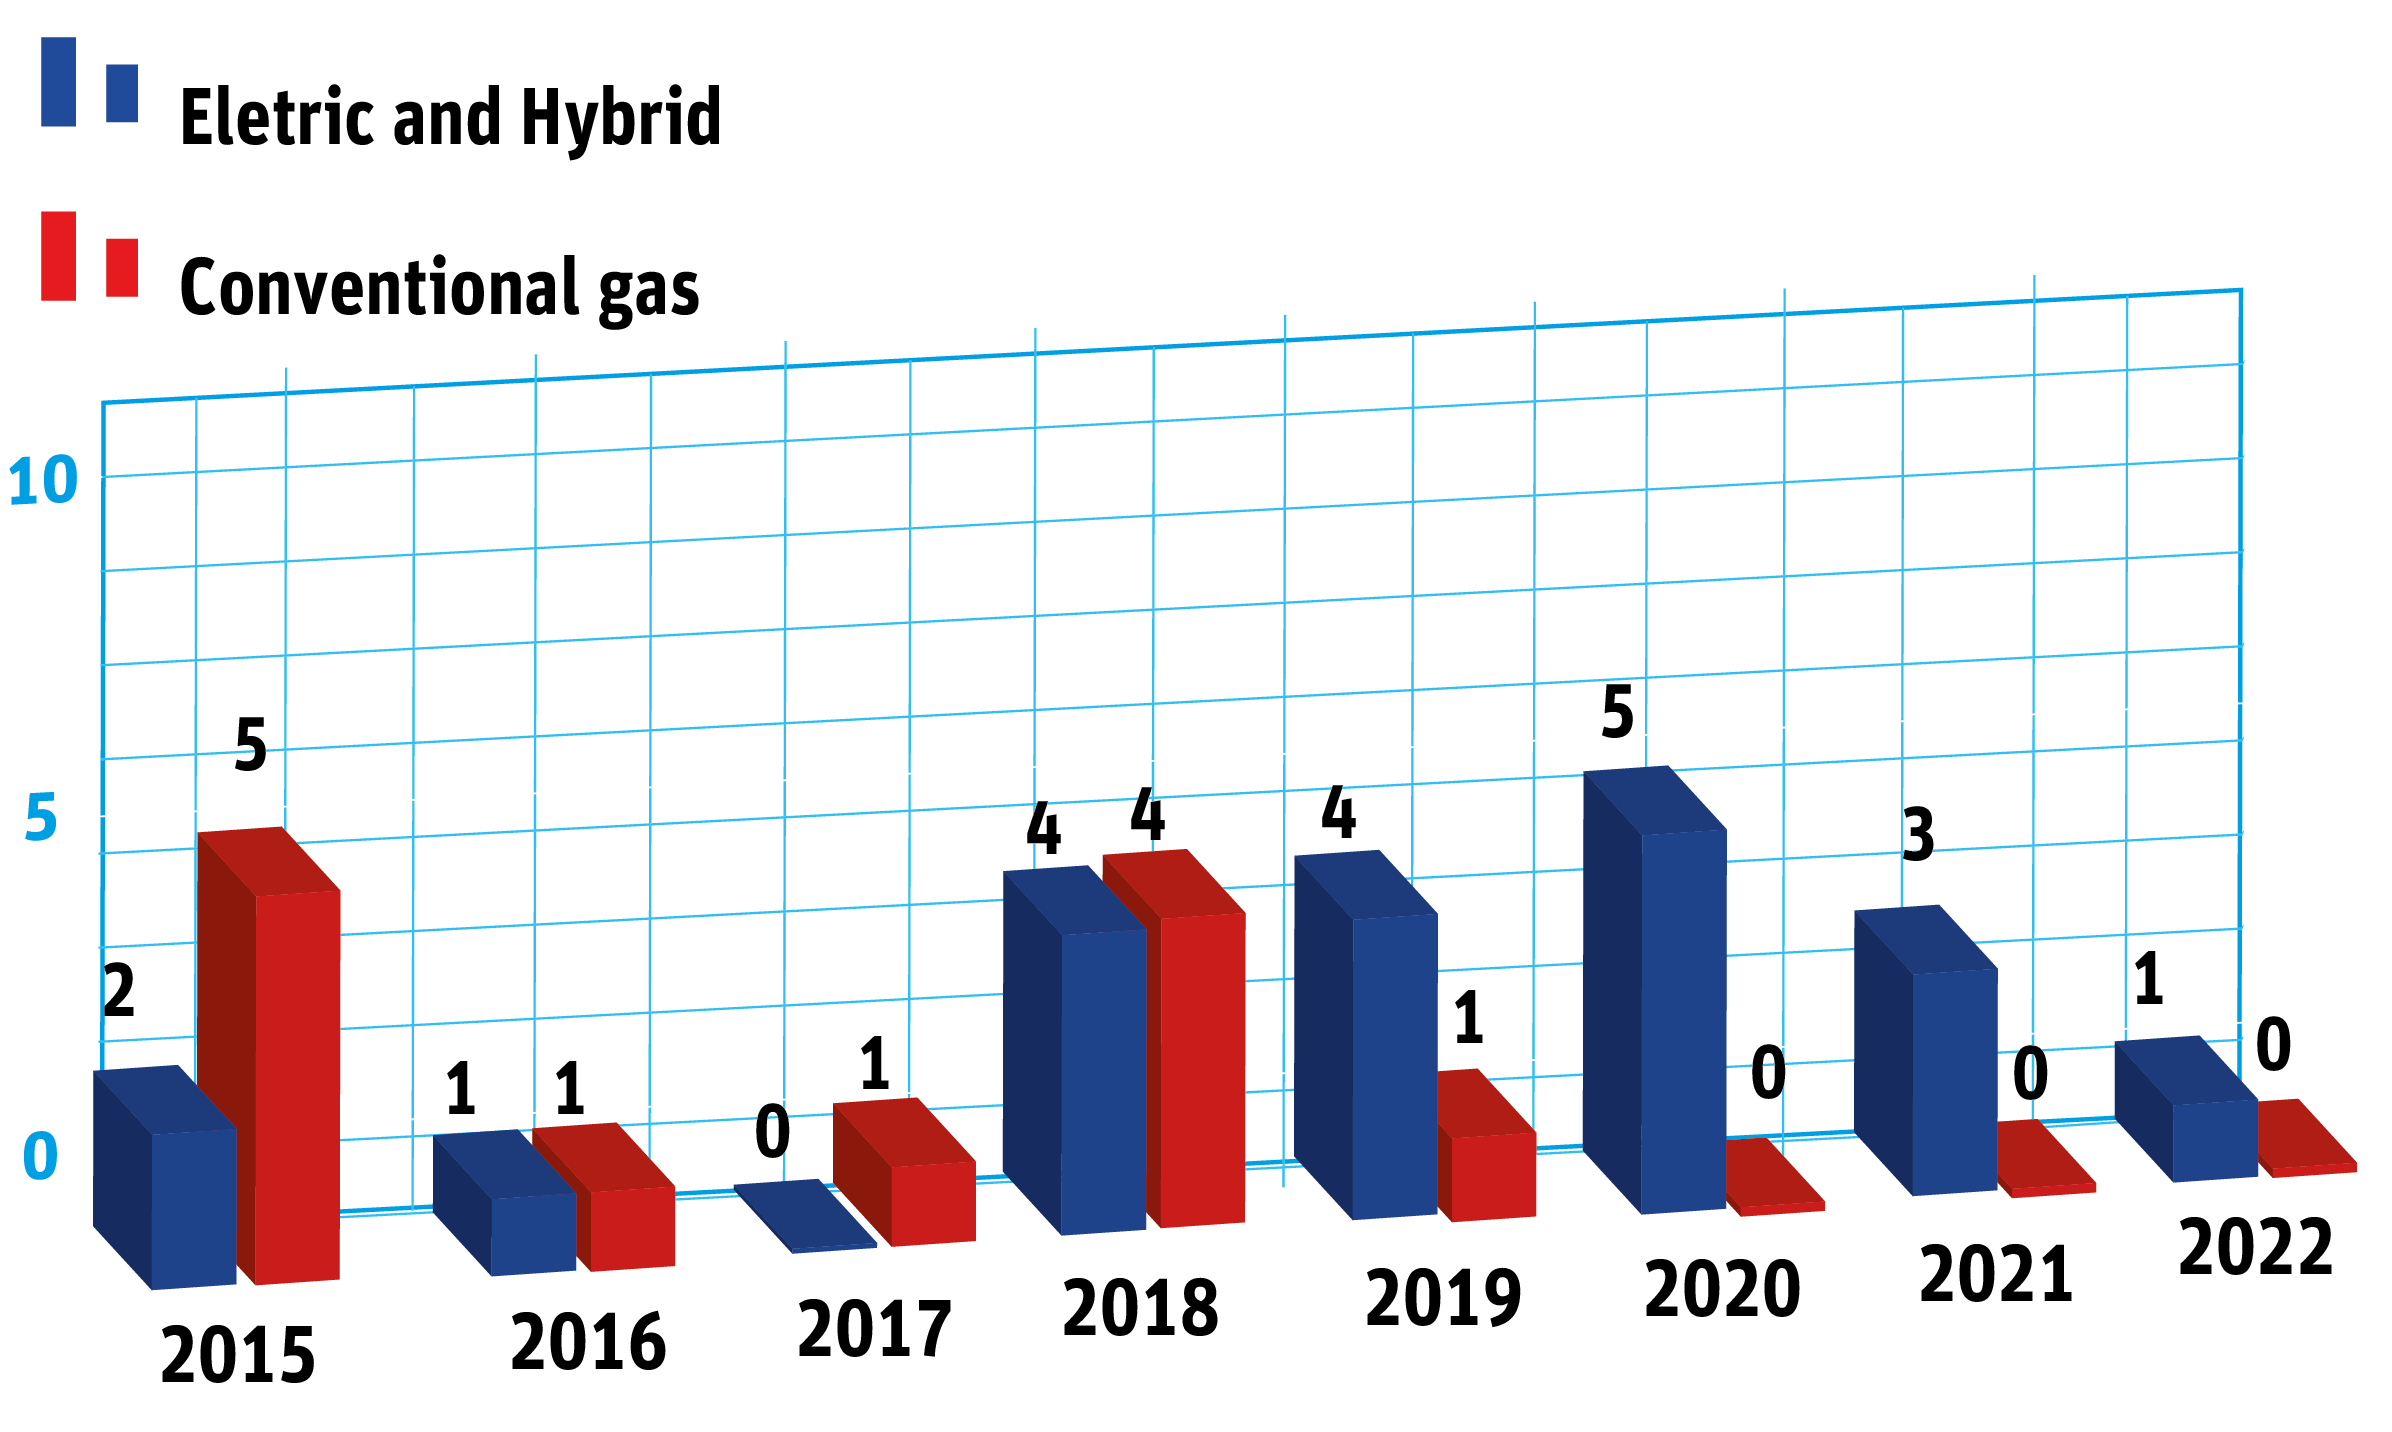
\includegraphics[width=\textwidth, keepaspectratio]{Prancheta 24.png} 
\end{figure}

\leavevmode\vspace{\baselineskip}%

\subsubsection {\textcolor{black}{\textbf{Mini Prototypes}}}

\leavevmode\vspace{0.1\baselineskip}%

Table \ref{table:miniP} shows the platform used for the mini ADV prototypes. The developers chose the do-it-yourself (DIY) car kit and the off-the-shelf remote control (RC) cars. The ones that were not in these two categories were classified as others.


\begin{table}[!ht]
  \centering
  \captionsetup{
    format=hang,
    justification=raggedright,
    singlelinecheck=false,
    skip=9pt,
  }
  \caption{\MakeUppercase{Type of vehicles used as a platform for the ADV mini prototype development}}
  \label{table:miniP}
  \def\arraystretch{1.5}
  \begin{tabularx}{\textwidth}{>{\raggedright\arraybackslash}p{2.0cm}>{\centering\arraybackslash}p{0.7cm}X}
    \arrayrulecolor{white}
    \rowcolor{white}
    \textbf{Type} & \textbf{Total} & \textbf{Papers} \\
    \arrayrulecolor{cor_tabela} \hline
    DIY Car Kit & \cellcolor{cor_tabela}\textbf{18} & \cellcolor{cor_tabela}\cite{azid2017,al2018,Sahu2019,Wang2019,roestam2019,Febbo2020,Fathy2020,el2020,10007388,9297973,albin2021design,JRC11091,Hartono_2020,10.1145/3556548.3559631,9690543,10.1007/978-3-030-55374-6_41,P2022108037,ILIE2020530}
 \\
    \arrayrulecolor{cor_tabela} \hline
    RC Cars 1:10 & \cellcolor{cor_tabela}\textbf{12} & \cellcolor{cor_tabela}\cite{Karaman2017,aguilar2017,Percinski2018,fayjie2018,deac2018,do2018,kwon2018,Gotlib2019,Walambe2019,Zhou2019,Valocky2019,Sajjad2020} \\
    \arrayrulecolor{cor_tabela} \hline
    Others & \cellcolor{cor_tabela}\textbf{6} & \cellcolor{cor_tabela}\cite{pannu2015,Bechtel2019,jain2018,Sun2019,chaitra2020,pehlivan2020} \\
    \arrayrulecolor{cor_tabela} \hline
  \end{tabularx}
\end{table}


The DIY car kits give more flexibility as researchers build their vehicles from scratch. A more advanced kit that would come even with the processing unit, battery, and sensors as the Elegoo Car Kit \cite{Febbo2020} was the choice of a few papers
\cite{Wang2019,Febbo2020,el2020}. On the other hand, a more basic kit was the one used by the researchers in the other five selected papers in this category\cite{azid2017,al2018,Sahu2019,roestam2019,Fathy2020}. It comes with the car chassis with wheels and steering system only \cite{Seeed}. All the other parts, like batteries, electric motors, and control systems, must be implemented. This approach gives a higher degree of freedom for the mini ADV development. However, it brings some extra work to set up the system properly, especially the car control system, meaning accelerating, braking, and steering.

The professional RC Cars 1:10 was the choice of most researchers. Buying a model with ready-made car controls removes the burden of implementing that and lets the development focus only on the autonomous details of the mini ADV prototype. Gotlib et al. \cite{Gotlib2019} developed a prototype for the F1 Tenth \cite{F1tenth} that promotes races between 1:10 autonomous vehicle prototypes worldwide and brings loads of information on how to build your own mini ADV prototype. Percinsky and Marcinkiewicz \cite{Percinski2018} and Blaga et al. \cite{deac2018} developed their prototype to enter the Carolo-Cup \cite{Carolo}. It was also an autonomous vehicle competition with 1:10 scale models.

Those mentioned competitions could be why most mini prototypes are professionally scaled 1:10 car models. In addition, the most used professional RC car found in the literature was the Traxxas models \cite{Traxxas}, which could be checked in some papers that mentioned the brand and in others by inspecting the model figure of the mini prototype.

The 1:10 scale, which means that the car is ten times smaller than the real size, gives enough room to put all the necessary processing units and sensors on it. Furthermore, the selection of professional RC models offers the advantage that the RC car is a replica of the real-size one in many aspects bringing the mini ADV prototype performance as close as possible to the implementation in real-size vehicles \cite{Walambe2019} \cite{Zhou2019}. Nevertheless, adaptations needed to be made, like swapping the radio control system with the autonomous one, installing the sensors, and distributing the battery power throughout all the included electric devices. The plastic body also needs to be removed.

Some mini ADV prototypes did not fit any category described in Table \ref{table:miniP}. Two papers did not mention details of the platform used for their prototypes \cite{chaitra2020}\cite{pannu2015}. Sun et al. \cite{Sun2019} employed a soccer bot as its prototype that would also participate in the Carolo Cup but in a different category than the ones mentioned before. Three other papers \cite{Bechtel2019,jain2018,pehlivan2020}
 applied a smaller size of an RC car for the prototype attempting to reduce its overall cost.

\subsection {\textbf{RQ2 What would be the hardware architecture and its characteristics for the upcoming ADV?}}

It is necessary to understand how every prototype works and its hardware configuration to visualize a general architecture of the ADV. Only some papers had diagrams to understand their architectures, so thoroughly inspecting the selected papers' topics was very important. Based on that, it was produced a generic hardware architecture for the ADV presented in Figure \ref{fig:hardware}. However, not every paper would give all details of its prototype such as the network protocol used or the computer configuration. Therefore, the results presented below reflect what was collected based on the available information .

\begin{figure}[ht]
  \centering
  
  % Caption setup for this specific figure
  \captionsetup{
     labelfont={bf,large},       % label (e.g., "Figure 1:") in bold and large
     textfont={bf,large},        % caption text in bold and large
     justification=raggedright,  % left-align the caption
     singlelinecheck=off         % force left alignment even for short captions
  }
  
  \caption{\MakeUppercase{ADV generic hardware architecture}}
  \label{fig:hardware}
  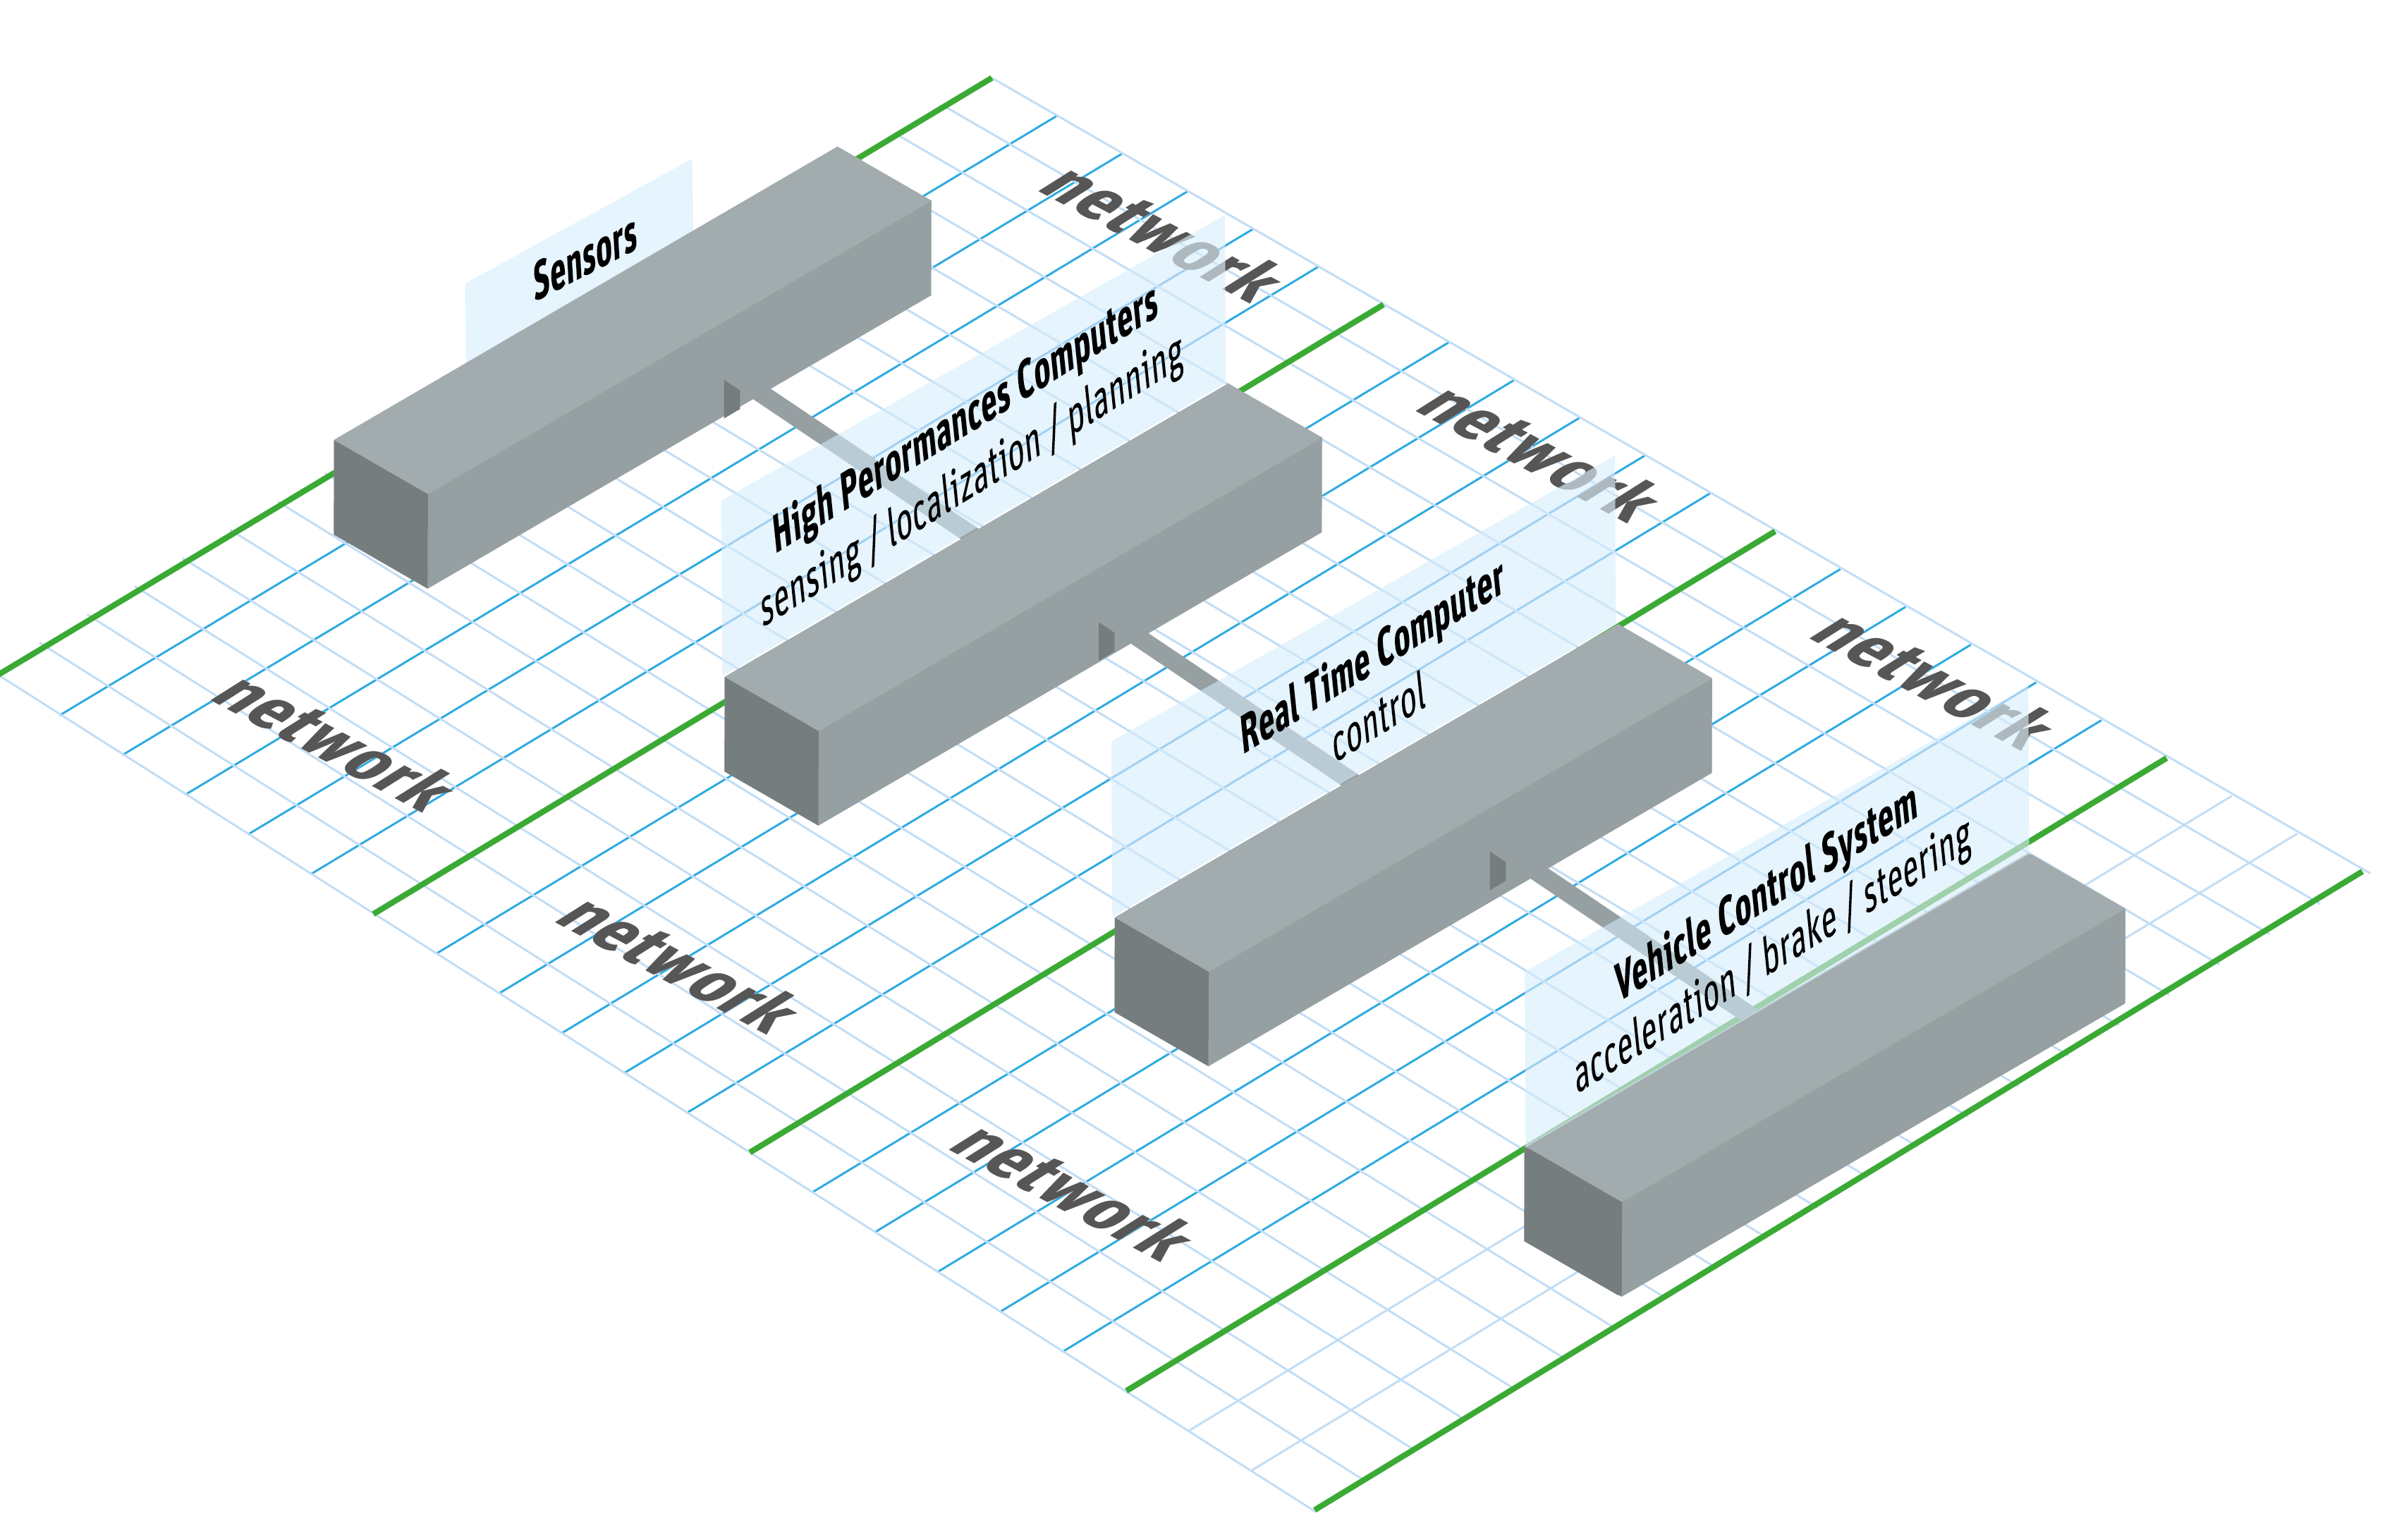
\includegraphics[width=\textwidth, keepaspectratio]{Prancheta 5 (2).png} 
\end{figure}

\subsubsection {\textcolor{black}{\textbf{Network Structure}}}

\leavevmode\vspace{0.1\baselineskip}%

\color{black}
The sensors are connected through a network to one or more computers. We found that in the real-size prototypes, the Ethernet and the CAN are the most used network protocols to connect the sensors \cite{Jo2015,Kunz2015,Kato2015,Broggi2015a,Broggi2015,Buechel2015,Aeberhard2015,Zong2018,Tas2018a,Munir2018,Aramrattana2018,Belcarz2018,Tang2018,Kessler2019,Betz2019,Reke2020,Angel2020,ORJUELA202015161,9544320,9359043,app11167225,electronics10192447}. Usually, the CAN network has the sensors the vehicle manufacturer provides as default, while the Ethernet network is used for inserting new sensors \cite{Kessler2019}. In addition, Munir et al. \cite{Munir2018} and Kessler et al. \cite{Kessler2019} required a USB protocol to connect their cameras for image processing, and Broggi et al. \cite{Broggi2015} required the same protocol to connect the LiDAR sensors to their prototype. 

\color{black}
The connection between the high processing and real-time computer was implemented using Ethernet, where three papers were using its high-speed variation, the Gigabit Ethernet \cite{Tang2018,Kessler2019,9359043}. The only exception was from Jo et al. \cite{Jo2015}, which interfaced the whole set of computers using the automotive FlexRay network, an alternative to the most traditional CAN network for inner vehicle sensor connections. The real-time computer and the vehicle control system were connected using the CAN network. It was a unanimous decision as the commercial vehicles have this network as default.

On the other hand, the mini prototypes relied on the USB protocol to connect their sensors, which is the pattern most used in the small-size sensors and computers applied in the mini ADV prototyping. Nevertheless, Wang et al. \cite{Wang2019} needed an Ethernet protocol due to the choice of a high-performance LiDAR for its prototype, the same applied in the real size ones.

\vspace{\baselineskip}

\subsubsection {\textcolor{black}{\textbf{Computing System for real-size prototypes}}}

\leavevmode\vspace{0.1\baselineskip}%

The computing system of the ADV could be divided into two parts: real-time computers and high-performance computers. The latter is responsible for the most computationally intense tasks, such as sensing, localization, and planning. In addition, it involves challenges like point cloud and convolutional neural network (CNN) processing within the time window required for safe and correct actions of the ADV prototype. Therefore, as described in Table \ref{table:hardware}, one or more computers were used for this purpose. 


\begin{table}[!ht]
  \centering
  \captionsetup{
    format=hang,
    justification=raggedright,
    singlelinecheck=false,
    skip=9pt,
  }
  \caption{\MakeUppercase{Number of Computers in Real-Size ADV Prototypes}}
  \label{table:hardware}
  \def\arraystretch{1.5}
  \begin{tabularx}{\textwidth}{>{\raggedright\arraybackslash}p{2.0cm}>{\centering\arraybackslash}p{0.7cm}X}
    \arrayrulecolor{white}
    \rowcolor{white}
    \textbf{Type} & \textbf{Total} & \textbf{Papers} \\
    \arrayrulecolor{cor_tabela} \hline
    \rule{0pt}{5.5ex}One & \cellcolor{cor_tabela}\textbf{7} & \cellcolor{cor_tabela}\cite{Kato2015,Bojarski2016,Zong2018,Belcarz2018,valera2019design,ORJUELA202015161,electronics10192447} \\
    \arrayrulecolor{cor_tabela} \hline
    \rule{0pt}{5.5ex}Two to Four & \cellcolor{cor_tabela}\textbf{18} & \cellcolor{cor_tabela}\cite{Kunz2015,Broggi2015a,Martin2016,Belbachir2017,Tas2018a,Munir2018,Aramrattana2018,Xu2018,Tang2018,Kessler2019,Betz2019,Marin-Plaza2019,Buyval2019,Reke2020,Angel2020,el2020,9359043,app11167225} \\
    \arrayrulecolor{cor_tabela} \hline
    \rule{0pt}{5.5ex}Five or more & \cellcolor{cor_tabela}\textbf{3} & \cellcolor{cor_tabela}\cite{Jo2015,Broggi2015,Buechel2015} \\
    \arrayrulecolor{cor_tabela} \hline
    \rule{0pt}{5.5ex}Not specified & \cellcolor{cor_tabela}\textbf{4} & \cellcolor{cor_tabela}\cite{Gupta2015,buchegger2018,9544320,9977411} \\
    \arrayrulecolor{cor_tabela} \hline
  \end{tabularx}
\end{table}



The real-time computer is responsible for the control functions of the vehicle: acceleration, brake, and steering. As the name says, it performs real-time actions critical for the correct response to the commands sent by high-performance computers. Every paper on Table \ref{table:hardware} with more than one computer on its prototype spared one specific computer for real-time applications. None of them employed more than one computer for that purpose.

As mentioned, the researchers combine one real-time computer and one or more high-performance computers, i.e., a heterogeneous architecture based on Central Processing Units (CPUs) and accelerators, e.g., Graphics Processing Units (GPUs), for the real-size ADV prototypes. However, there are some exceptions.

Valera et al.  \cite{valera2019design} designed from scratch a tubular go-kart to drive autonomously. They applied a Beaglebone cyan \cite{BeagleBone} as the vehicle computing unit responsible for processing camera and LiDAR signals and controlling the vehicle. It was an ambitious project to process all this information. This computer is equivalent to a Raspberry Pi 3 \cite{RaspberryPI}  or a Jetson Nano \cite{JetsonNano}, i.e., computers with limited processing power. The paper has no information about its real performance as only simulation data was presented even though a prototype was constructed.

Two papers adopted the Nvidia Drive Computers for autonomous drive \cite{NvidiaDrive} as their prototype single computers. It is a computer series comprising many computing devices (GPU and CPU) and integrated memory designed for autonomous applications. A paper from the Nvidia Corporation \cite{Bojarski2016} employed the discontinued Nvidia Drive PX as the vehicle computer in an end-to-end approach. It means that the vehicle control commands would be based exclusively on the cameras around the vehicles without any other sensors involved. This approach was followed by only some of the researchers, as could be seen in the selected papers.

Belcarz et al. \cite{Belcarz2018} and Chung and Yang \cite{electronics10192447} also employed the discontinued Nvidia Drive PX2 as their prototype computer. However, they did so in an architectural fashion close to the other researcher´s prototypes, relying not only on the camera but on a set of sensors such as LiDAR and GPS to control the autonomous vehicle. Additionally, Kessler et al. \cite{Kessler2019} and Betz et al. \cite{Betz2019} utilized the Nvidia Drive PX2 as its high-performance computer to process perception and planning tasks leaving other tasks like vehicle control to other computers.

 Kato et al. \cite{Kato2015} used a single computer with different combinations of Intel CPUs and Nvidia GPUs in their prototype. They argued that running all necessary tasks for autonomous driving in less than 100ms would need an improvement in the available GPUs by a factor of two. Zong et al. \cite{Zong2018} proposed a similar approach. However, they concluded that a computer with only a CPU would not be the best choice and believed that using an embedded computer like the ones from Nvidia could be the future trend for the ADV.

One different approach was to apply a distributed computing architecture compared to the centralized computing architecture presented in Figure \ref{fig:hardware}. It was considered a distributed architecture the ADV prototypes with five or more computing units. 

Jo et al. \cite{Jo2015} have fifteen computers in their prototype, two industrial computers (sensor fusion and planning) and another for vision processing, which compose the high-performance computing system. They employed one real-time computer for vehicle control algorithms processing but left the actuation to a separate Electronic Computing Unit (ECU) based on a 32-bit microcontroller. Other tasks, such as detection, positioning, and vehicle state, were distributed in the available MCUs.

In a similar distributed approach, Broggi et al. \cite{Broggi2015} developed a prototype with twenty-one computers, including seventeen computers equipped with an Intel i7 CPU. This prototype relies on image processing with thirteen stereo cameras, a highly intense computational task. So each computer is mapped to process one to two image sensors connected in a single network. Then, some application computers would get this processed data and execute the other tasks necessary for the autonomous vehicle to travel.

FPGAs were the choice of Buechel et al. \cite{Buechel2015} prototype. The system has five computers, each composed of two Xilinx Zynq FPGA and a Dual ARM CPU connected in a network. The author states that its architecture would be dramatically simplified if all components had a self-developed network protocol. However, these distributed architecture prototypes were from 2015, and the other selected prototypes from the subsequent years had not chosen that approach.

There is a trend to reduce the number of computers in commercial vehicles. Instead of having several ECU for each vehicle system, it will have a few computers to control every aspect of the ADV, moving towards a software-defined vehicle with less complexity and lower overall cost \cite{Aptiv}.

The Intel i7 CPU is the most used computer processor among the papers that described their prototype computing platform \cite{Kunz2015,Kato2015,Broggi2015,Buechel2015,Martin2016,Zong2018,Kessler2019,Betz2019,Marin-Plaza2019,Reke2020}.
This could be a sign that even the researchers that did not disclose their computer details, identifying it only as a PC, might use it as well. Nevertheless, it was identified some other attempts to use the discontinued Intel Core 2 Duo \cite{Jo2015} \cite{Broggi2015a}, Intel Xeon \cite{Tas2018a}, and an Intel i5 \cite{Aramrattana2018}.
 
 Another popular choice among researchers was the Nvidia GPU-based embedded computers for artificial intelligence \cite{Tang2018}
\cite{Buyval2019}
 and for autonomous driving \cite{Bojarski2016,Belcarz2018,Kessler2019,Betz2019}
employed alone or together with other computing devices. These devices provide powerful embedded GPUs to accelerate artificial algorithms processing. In addition, only a few prototypes give details about GPU configuration when using an Intel CPU in their development \cite{Kato2015,Tas2018a,Buyval2019,Angel2020}.

One more often used device as a real-time computer is the dSpace Micro Autobox, which was the choice of some developed real-size prototypes \cite{Kato2015,Tas2018a,Buyval2019,Angel2020}. This real-time system is designed for rapid prototyping of vehicle applications with many network protocols included and robust enough to be in the harsh vehicle environment \cite{dSpace}. The authors applied this device to connect to the commercial vehicle CAN bus to override the original system control commands with their control strategy developed on the Micro Autobox embedded PC running Linux operational system.

The hardware details of the mini prototypes could be seen in every selected paper.
Raspberry Pi 3, Nvidia Jetson series (TX1 \cite{Karaman2017,kwon2018,Zhou2019}
, TX2\cite{fayjie2018}
\cite{Wang2019},
 and Nano \cite{Febbo2020}) for high-performance tasks processing and Arduino (Uno and Mega\cite{Wang2019})
 for the real-time control were the choices of most papers, although there were prototypes with one computer and others with two. These details can be seen in Tables \ref{table:mini} and \ref{table:minicomp}. It is important to note that all computers employed had one or more ARM-based CPUs, with a GPU included for high-performance processing.



\begin{table}[!ht]
  \centering
  \captionsetup{
    format=hang,
    justification=raggedright,
    singlelinecheck=false,
    skip=9pt,
  }
  \caption{\MakeUppercase{Number of Computers in the Mini ADV Prototypes}}
  \label{table:mini}
  \def\arraystretch{1.5}
  \begin{tabularx}{\textwidth}{>{\raggedright\arraybackslash}p{2.0cm}>{\centering\arraybackslash}p{0.7cm}X}
    \arrayrulecolor{white}
    \rowcolor{white}
    \textbf{Type} & \textbf{Total} & \textbf{Papers} \\
    \arrayrulecolor{cor_tabela} \hline
    One & \cellcolor{cor_tabela}\textbf{17} & \cellcolor{cor_tabela}\cite{pannu2015,Karaman2017,azid2017,fayjie2018,deac2018,kwon2018,Sahu2019,Zhou2019,roestam2019,Sajjad2020,el2020,10007388,9297973,albin2021design,10.1145/3556548.3559631,9690543,10.1007/978-3-030-55374-6_41} \\
    \arrayrulecolor{cor_tabela} \hline
    Two & \cellcolor{cor_tabela}\textbf{18} & \cellcolor{cor_tabela}\cite{aguilar2017,Bechtel2019,Percinski2018,al2018,jain2018,do2018,Gotlib2019,Walambe2019,Sun2019,Wang2019,Valocky2019,Febbo2020,Fathy2020,chaitra2020,pehlivan2020,ILIE2020530,JRC11091,Hartono_2020} \\
    \arrayrulecolor{cor_tabela} \hline
    Not specified & \cellcolor{cor_tabela}\textbf{1} & \cellcolor{cor_tabela}\cite{P2022108037} \\
    \arrayrulecolor{cor_tabela} \hline
  \end{tabularx}
\end{table}






\begin{table}[!ht]
  \centering
  \captionsetup{
    format=hang,
    justification=raggedright,
    singlelinecheck=false,
    skip=9pt,
  }
  \caption{\MakeUppercase{Hardware Choice for the Mini ADV Prototypes}}
  \label{table:minicomp}
  \def\arraystretch{1.5}
  \begin{tabularx}{\textwidth}{>{\raggedright\arraybackslash}p{3cm}>{\centering\arraybackslash}p{0.7cm}X}
    \arrayrulecolor{white}
    \rowcolor{white}
    \textbf{Type} & \textbf{Total} & \textbf{Papers} \\
    \arrayrulecolor{cor_tabela} \hline
    \textcolor{black}{Raspberry Pi 3} & \cellcolor{cor_tabela}\textbf{17} & \cellcolor{cor_tabela}\cite{pannu2015,aguilar2017,Bechtel2019,al2018,deac2018,jain2018,do2018,Walambe2019,Sahu2019,Sun2019,Sajjad2020,Fathy2020,el2020,chaitra2020,pehlivan2020,ILIE2020530} \\
    \arrayrulecolor{cor_tabela} \hline
    Nvidia Jetson Series & \cellcolor{cor_tabela}\textbf{9} & \cellcolor{cor_tabela}\cite{Karaman2017,kwon2018,Zhou2019,fayjie2018,Wang2019,Febbo2020,10007388,9297973,10.1145/3556548.3559631} \\
    \arrayrulecolor{cor_tabela} \hline
    Arduino & \cellcolor{cor_tabela}\textbf{16} & \cellcolor{cor_tabela}\cite{aguilar2017,azid2017,al2018,jain2018,do2018,Walambe2019,Wang2019,Valocky2019,roestam2019,Febbo2020,Fathy2020,chaitra2020,albin2021design,JRC11091,Hartono_2020,10.1007/978-3-030-55374-6_41} \\
    \arrayrulecolor{cor_tabela} \hline
    Others & \cellcolor{cor_tabela}\textbf{6} & \cellcolor{cor_tabela}\cite{Percinski2018,Gotlib2019,Sun2019,pehlivan2020,P2022108037,9690543} \\
    \arrayrulecolor{cor_tabela} \hline
  \end{tabularx}
\end{table}

\vspace{\baselineskip}

\subsubsection {\textcolor{black}{\textbf{Computing System for mini prototypes}}}

\leavevmode\vspace{0.1\baselineskip}%

The architecture choice of the mini prototypes was based on the number of high-performance processing functions to be implemented and the number of sensors to be connected. The ones with only one computer would accumulate high-performance and real-time tasks. The prototypes with only the Raspberry Pi or Arduino as a computing unit \cite{pannu2015,azid2017,deac2018,Sahu2019,roestam2019,Sajjad2020,el2020} would have fewer functions if compared with the prototypes implemented with the more powerful Nvidia Jetson series computers\cite{Karaman2017,fayjie2018,kwon2018,Zhou2019}. However, the first choice made the whole prototype less expensive.

The mini prototypes with two computers would follow the real-size prototypes fashion by separating the vehicle control from the high-performance tasks to ensure real-time actions for the commands issued by the high-performance computer. The microcontroller Arduino was the most used as a real-time computer as it emulates the use of an ECU applied on real-size vehicles. As mentioned before, the other vehicle tasks were implemented by a single-board computer.

Some slightly different approaches were found as well. Percinski and Marcinkiewicz \cite{Percinski2018} chose the single computer board Odroid XU4 \cite{odroid} for high-performance processing and an open source project AnyFCF7 \cite{ANYFCF7} for real-time motor control. In addition, a second prototype with the same hardware architecture was designed by Gotlib et al. \cite{Gotlib2019}. Furthermore, Pehlivan et al. \cite{pehlivan2020} opted for a different real-time vehicle control computer, which was the Robot Hat \cite{RobotHat}. That computer was designed specifically for robot movement control, which suits the mini ADV applications.

Due to the high-intense computational task of training a neural network, three papers opted to use an additional desktop or laptop computer for network training \cite{Bechtel2019,do2018,pehlivan2020}. It was not counted as a third computer, as those were off the prototype body. All of them were using a Raspberry Pi 3, which was unsuitable for the network training or would take too long to conclude.

\subsection{\textbf{RQ3  What would be the software architecture and its characteristics for the upcoming ADV?}}

\vspace{\baselineskip}

\subsubsection {\textcolor{black}{\textbf{Software Architecture}}}

\leavevmode\vspace{0.1\baselineskip}%

After inspecting every selected paper, it was possible to draw the generic software architecture for the ADV represented in Figure \ref{fig:software}. It is important to mention that not every ADV prototype had all functions and sensors represented in that generic architecture. Nevertheless, the prototypes would have at least one feature or sensor. 

The prototypes made of commercial vehicles, what was almost every full-size ADV prototype mapped, had a complete software architecture. In contrast, the mini prototypes mostly had a concise architecture due to the lack of processing power. Nevertheless, the prototypes from Wang et al. \cite{Wang2019} and Zhou et al. \cite{Zhou2019} were among the mini prototypes that developed a complete software architecture similar to the architecture of the full-size ones.

The processing system, as mentioned before, is composed of one or more computers with different characteristics and configurations from each selected prototype. Although various computer configurations exist, the operating system and middleware are practically a unanimous choice among researchers.

\begin{figure}[ht]
  \centering
  
  % Caption setup for this specific figure
  \captionsetup{
     labelfont={bf,large},       % label (e.g., "Figure 1:") in bold and large
     textfont={bf,large},        % caption text in bold and large
     justification=raggedright,  % left-align the caption
     singlelinecheck=off         % force left alignment even for short captions
  }
  
  \caption{\MakeUppercase{ADV generic software architecture}}
  \label{fig:software}
  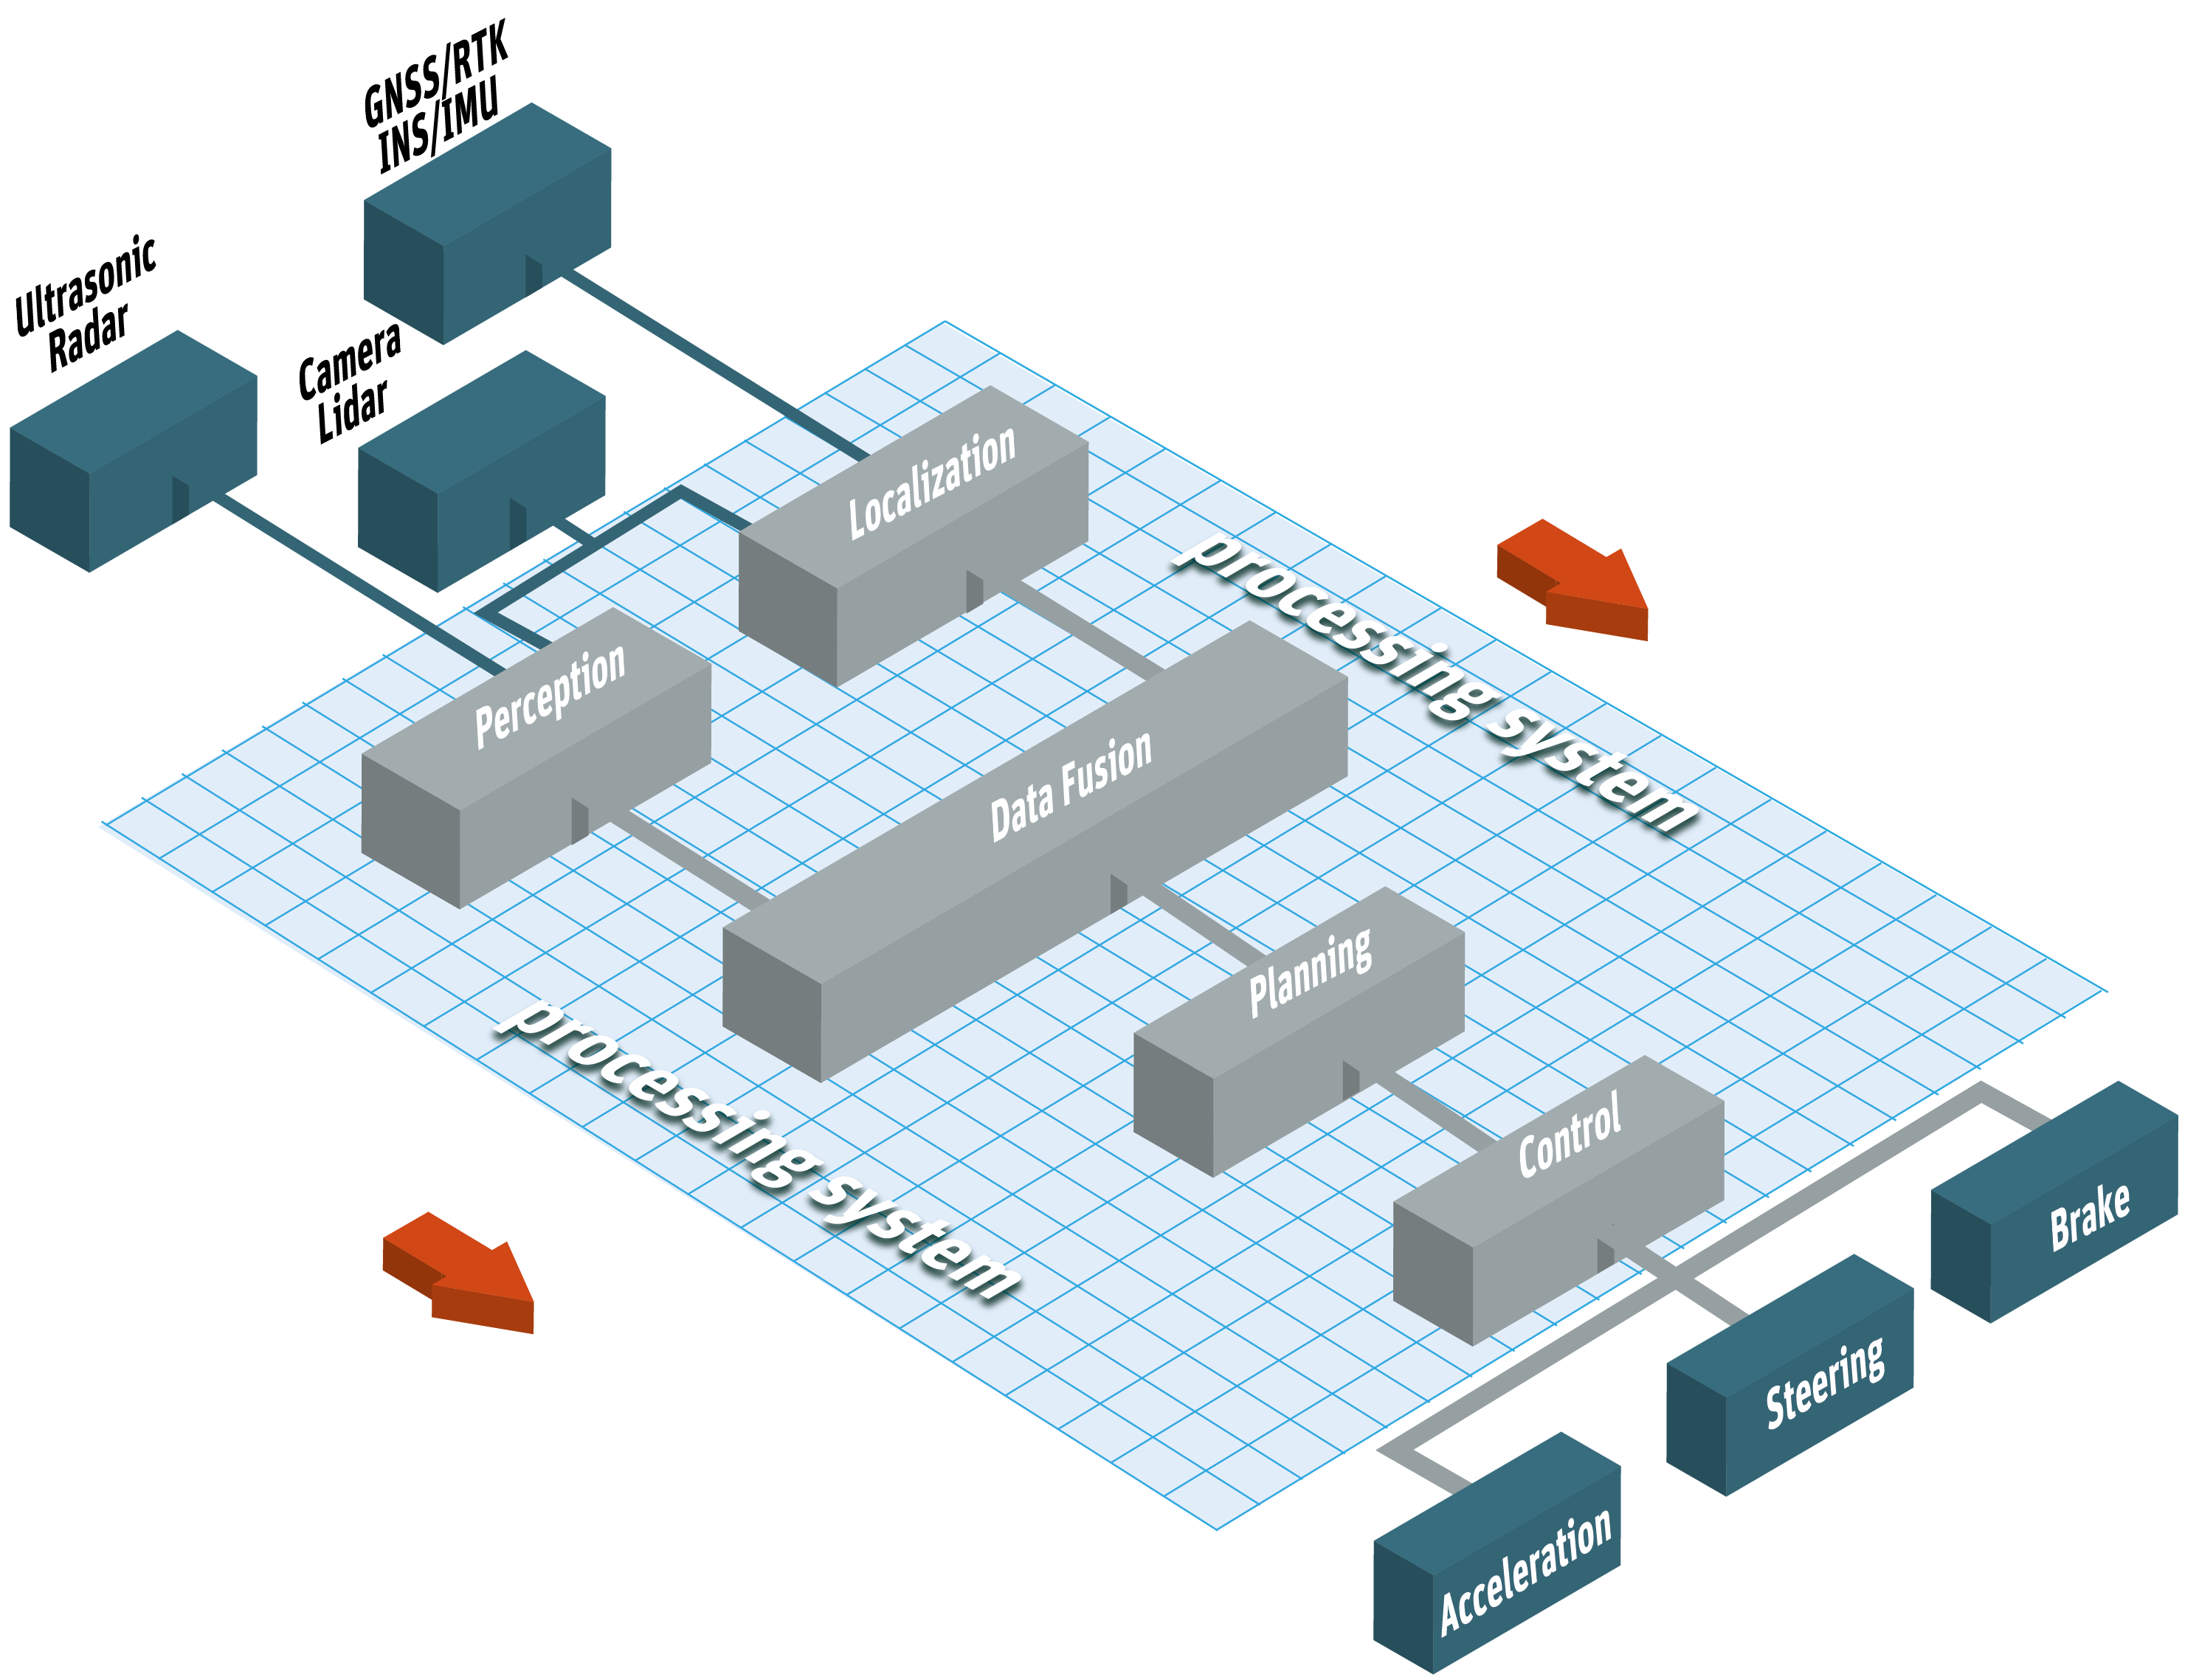
\includegraphics[width=\textwidth, keepaspectratio]{Prancheta 1 (1).png} 
\end{figure}


\vspace{\baselineskip}

\subsubsection {\textcolor{black}{\textbf{Middleware and Software Libraries}}}

\leavevmode\vspace{0.1\baselineskip}%


The most used software for ADV development in both mini and real-size prototypes was the Robot Operating System (ROS),\cite{Gupta2015,Martin2016,Tas2018a,Munir2018,Belcarz2018,Betz2019,Marin-Plaza2019,valera2019design,Reke2020,Angel2020,el2020,Karaman2017,al2018,Gotlib2019,Zhou2019,Wang2019,ILIE2020530,app11167225,10.1145/3556548.3559631}. ROS is an open-source midlleware \cite{Angel2020} or a meta operating system \cite{ros} developed for robotic applications such as autonomous vehicles. It provides libraries and communication layers for autonomous driving tasks \cite{Betz2019}. The tasks are separated into nodes, modularizing the software development and creating independence between different ADV functions. Although ROS provides some operating system functions like hardware abstraction, it must run over an operation system, which Ubuntu Linux is recommended by the ROS developers \cite{ros}.


In contrast, Kessler et al. \cite{Kessler2019} and Buyval et al. \cite{Buyval2019} chose the open-source Apollo framework for autonomous driving \cite{Apollo}. Apollo is an extended version of the ROS framework with decentralized node control and improved communications capabilities \cite{Kessler2019}. Buyal et al. have found many disadvantages in the planning and control modules of the Apollo firmware, so they decided to replace both with a Model Predictive Control module. Kato et al. \cite{Kato2015} used the Autoware framework \cite{Autoware} as the core of their prototype´s software, and El-Tawab et al. \cite{el2020autonomous} applied the mapping and localization algorithm provided by that. Autoware is based on ROS and provides a variety of modules for autonomous vehicle tasks \cite{Betz2019}. 

Furthermore, some researchers have decided to develop solutions to overcome some weak points of the ROS middleware. For example, Tang et al. \cite{Tang2018} stated that ROS is unsuitable for low-power edge computing systems, so they developed the $\pi$-OS middleware to overcome the high communication overhead and the large number of library dependencies imposed by ROS. The authors concluded that their middleware had $50\%$ lower latency than ROS. 

In order to overcome the same restrictions stated before, Zhang et al. \cite{Zhang2018} developed the Project Cocktail, a data transmission module to manage and improve system communications by dealing with data flows as binary streams, being independent of data format transmissions between network peers. The authors' module could outperform ROS with communication latency, which was crucial for the ADV system to achieve real-time performance.

Xu et al. \cite{Xu2018} developed the PACPUS middleware. Compared to ROS and other middleware, it focused on the execution performance of the software. It allows dynamic loading and networking distribution of components at execution time. Gold was also a firmware developed by Broggi et al. \cite{Broggi2015} \cite{Broggi2015a} and applied in their two ADV prototypes. It has similar characteristics to ROS and was developed in C++ language.

To overcome some of the downfalls, ROS has evolved to ROS2, a second version of the most popular firmware for autonomous driving. For example, the prototyped developed by Reke et al. \cite{Reke2020} employed ROS2. The author stated that the second version of the middleware would keep the modularity of the first version and bring real-time performance as an improvement.

Many prototype developers used two relevant software libraries, mostly in the mini ADVs, independent of the middleware in use. These were OpenCV, employed in \cite{Jo2015,Kato2015,pannu2015,deac2018,jain2018,Sahu2019,Zhou2019,Sun2019,chaitra2020,valera2019design,pehlivan2020,Sajjad2020,fayjie2018,al2018,Wang2019,Febbo2020} and TensorFlow, employed in \cite{Bechtel2019,do2018,chaitra2020,pehlivan2020,fayjie2018,Wang2019,Febbo2020,valera2019design} for image processing and classification. OpenCV is an open-source computer vision library that can handle images and videos \cite{jain2018} and is mostly used in the ADV for image collection and processing. TensorFlow is a library that allows to build and train a deep learning model \cite{chaitra2020} and is mostly used to classify images captured by the ADV. The OpenCV is progressing in its machine learning functionalities, but developers prefer to build the deep learning model on TensorFlow and import it to be applied by the OpenCV.

\subsection {\textbf{RQ4 Which would be the sensor set necessary for a   fully functional ADV?}}

 Figure \ref{fig:software} presents the six main sensors necessary to build an autonomous vehicle. Over the selected papers, not all prototypes would use all sensors. However, there are some real-size prototypes with the full set of sensors 
\cite{Tas2018a,Belcarz2018,Kessler2019,Betz2019,ORJUELA202015161,9544320,9359043}. There are fairly complex mini prototypes  as well \cite{Percinski2018,fayjie2018,jain2018,Zhou2019,Wang2019,roestam2019,el2020}, but none had the full set of sensors. Table \ref{table:sensor} shows what sensors were applied in each prototype.



\begin{table}[!ht]
  \centering
  \captionsetup{
    format=hang,
    justification=raggedright,
    singlelinecheck=false,
    skip=9pt,
  }
  \caption{\MakeUppercase{Sensor Utilization per Prototype}}
  \label{table:sensor}
  \def\arraystretch{1.5}
  \begin{tabularx}{\textwidth}{>{\raggedright\arraybackslash}p{2.0cm}>{\centering\arraybackslash}p{0.7cm}X}
    \arrayrulecolor{white}
    \rowcolor{white}
    \textbf{Type} & \textbf{Total} & \textbf{Papers} \\
    \arrayrulecolor{cor_tabela} \hline
    \rule{0pt}{4.5ex}LiDAR & \cellcolor{cor_tabela}\textbf{31} & \cellcolor{cor_tabela} 
\cite{Gupta2015,Kato2015,Broggi2015a,Broggi2015,Buechel2015,Belbachir2017,Zong2018,Tas2018a,Munir2018,Belcarz2018,Xu2018,buchegger2018,Kessler2019,Betz2019,Marin-Plaza2019,valera2019design,Angel2020,el2020,Karaman2017,aguilar2017,Percinski2018,fayjie2018,Wang2019,Gotlib2019,Zhou2019,Buyval2019,ILIE2020530,ORJUELA202015161,app11167225,10.1145/3556548.3559631,electronics10192447}

\\
    \arrayrulecolor{cor_tabela} \hline
    \rule{0pt}{4.5ex}Camera & \cellcolor{cor_tabela}\textbf{48} & \cellcolor{cor_tabela}
\cite{Jo2015,Kunz2015,Kato2015,Broggi2015a,Broggi2015,Buechel2015,Bojarski2016,Belbachir2017,Zong2018,Tas2018a,Munir2018,Belcarz2018,Kessler2019,Betz2019,Marin-Plaza2019,valera2019design,Reke2020,Angel2020,el2020,pannu2015,Karaman2017,Bechtel2019,Percinski2018,fayjie2018,deac2018,jain2018,do2018,kwon2018,Sahu2019,Zhou2019,Sun2019,Wang2019,roestam2019,Sajjad2020,Febbo2020,Fathy2020,chaitra2020,pehlivan2020,Buyval2019,ILIE2020530,ORJUELA202015161,10007388,9297973,albin2021design,app11167225,10.1145/3556548.3559631,9690543,electronics10192447}



 \\
\arrayrulecolor{cor_tabela} \hline
    \rule{0pt}{4.5ex}Radar & \cellcolor{cor_tabela}\textbf{14} & \cellcolor{cor_tabela} 
\cite{Kunz2015,Broggi2015a,Buechel2015,Zong2018,Tas2018a,Aramrattana2018,Betz2019,Kessler2019,Belcarz2018,Reke2020,Broggi2015,Buyval2019,electronics10192447}

 \\
\arrayrulecolor{cor_tabela} \hline
    \rule{0pt}{4.5ex}Ultrasonic & \cellcolor{cor_tabela}\textbf{21} & \cellcolor{cor_tabela}
\cite{Kunz2015,Tas2018a,Aramrattana2018,Belcarz2018,Kessler2019,Betz2019,pannu2015,al2018,Valocky2019,roestam2019,Sajjad2020,el2020,Buechel2015,Marin-Plaza2019,pehlivan2020,Sahu2019,azid2017,ORJUELA202015161,JRC11091,Hartono_2020,10.1145/3556548.3559631}


 \\
 
    \arrayrulecolor{cor_tabela} \hline
    \rule{0pt}{4.5ex}GNSS/RTK & \cellcolor{cor_tabela}\textbf{27} & \cellcolor{cor_tabela} 
\cite{Gupta2015,Jo2015,Kunz2015,Kato2015,Broggi2015a,Broggi2015,Buechel2015,Belbachir2017,Zong2018,Tas2018a,Munir2018,Aramrattana2018,Belcarz2018,Xu2018,buchegger2018,Kessler2019,Reke2020,Angel2020,el2020,aguilar2017,deac2018,roestam2019,Buyval2019,al2018,Betz2019,Marin-Plaza2019,ORJUELA202015161}


 \\
 
    \arrayrulecolor{cor_tabela} \hline
    \rule{0pt}{4.5ex}INS/IMU & \cellcolor{cor_tabela}\textbf{26} & \cellcolor{cor_tabela}
\cite{Jo2015,Belbachir2017,Zong2018,Tas2018a,Belcarz2018,Tang2018,buchegger2018,Reke2020,Angel2020,el2020,Karaman2017,Percinski2018,fayjie2018,Gotlib2019,Zhou2019,Betz2019,Buechel2015,Marin-Plaza2019,Buyval2019,Munir2018,Broggi2015,Broggi2015a,deac2018,Kessler2019,ILIE2020530,ORJUELA202015161}

 \\
   \arrayrulecolor{cor_tabela} \hline
  \end{tabularx}
\end{table}



\vspace{\baselineskip}

\subsubsection {\textcolor{black}{\textbf{LiDAR}}}

\leavevmode\vspace{0.1\baselineskip}%

The LiDAR (light detection and ranging) is an important sensor that can be used for perception and localization. It produces point cloud data that can be processed to map the environment, locate the ADV, detect objects, and measure the distance from them \cite{Kato2015}. It can be processed in popular libraries such as OpenCV. However, this sensor is the barrier to popularizing the ADV due to its high cost, which can get up to 75,000 dollars \cite{Lin2018}. This makes prototype developers search for alternatives for that sensor, like using only cameras as proposed by Tang et al. \cite{Tang2018}. However, Kessler et al. \cite{Kessler2019} consider the LiDAR a mandatory sensor for autonomous vehicles.

There are two types of LiDAR. The 2d LiDAR is applied to object detection and distance measurement. The 3d LiDAR increases the sensing capabilities by measuring height, width, and depth, which is necessary to identify objects' characteristics. The simultaneous localization and mapping (SLAM) algorithm is a popular application that uses the 3d LiDAR to make a real-time environment map with detailed object information.

In order to reduce the cost, mini prototypes use a 2d LiDAR with a price starting from 100 dollars for 2d mapping, object detection, and ranging. In addition, it can have its data merged with a camera to get similar functions to the expensive 3d LiDAR \cite{fayjie2018}. The cited manufacturers for LiDAR were Velodyne, Hokuyo, Ibeo, Sick, and Slamtec.


\vspace{\baselineskip}

\subsubsection {\textcolor{black}{\textbf{Camera}}}

\leavevmode\vspace{0.1\baselineskip}%

The camera can be applied to localization and perception as well. We found various camera types applied to ADV, ranging from static and moving, monochrome and color, stereo, spherical, and smart cameras. Some prototypes have very low-resolution cameras with 640 x 480 pixels \cite{Bechtel2019} in contrast to powerful cameras that could get up to 4416 x 1242 \cite{Karaman2017}, which is higher than the Full HD resolution commonly seen on television transmissions.

The most often camera applications throughout the selected paper are to detect objects following their type classification. However, some prototypes use the camera images as the only system sensor for obstacle avoidance without classification in an end-to-end approach,
 driving the ADV only with the camera information \cite{Bechtel2019,fayjie2018,jain2018,do2018,kwon2018,Valocky2019,Bojarski2016}. The camera used for only detection was applied when it was inserted in a real-size prototype with more sensors \cite{Bojarski2016,Belbachir2017,Munir2018,Betz2019,Marin-Plaza2019,el2020,al2018} or with the only function of object avoidance in mini prototypes with limited computer resources \cite{pannu2015}
\cite{Percinski2018}. In addition, some prototypes employed the camera also for mapping the environment in SLAM applications\cite{Tang2018,Martin2016,Zhou2019,Wang2019}.


Monochrome or color cameras detect road lanes, traffic signals, pedestrians, and any road objects. Furthermore, more complex cameras were also applied in the ADV development. The stereotype camera, employed by some authors \cite{Broggi2015a,Broggi2015,Martin2016,Belcarz2018,Marin-Plaza2019,el2020,fayjie2018,Fathy2020,Tas2018a,Karaman2017,roestam2019}, has two lenses, collecting two separated images that, when matched and compared, can provide depth information through a disparity map \cite{Marin-Plaza2019}. The main advantage of this approach is that it is possible to know the exact distance from each obstacle detected, which cannot be done with monocular cameras.

Moreover, Kato et al. \cite{Kato2015} used a camera system mounted on the ADV roof that could provide a 360 view of spherical images. Reke et al. \cite{Reke2020} employed the Intel Mobileye camera system with the main advantage of processing its images, saving processing power from the computing system of the ADV. 
 
The main camera manufacturers for the ADV application found were Baumer, Flir, Point Grey, IDS, Seknonix, Zed, and Kurokesu. However, the most popular mini ADV prototype was the PiCamera.

\vspace{\baselineskip}

\subsubsection {\textcolor{black}{\textbf{Radar and Ultrassonic}}}

\leavevmode\vspace{0.1\baselineskip}%
 
The radar is used for obstacle detection in the area surrounding the vehicle in short, medium, and long ranges as part of the perception system \cite{Tas2018a}. It gives precise range and velocity measurements compared to cameras at the cost of less accurate classification capabilities \cite{Kunz2015}. Thus, it is often used with other sensors such as LiDAR, Cameras, and GNSS systems. However, the most common application was as a long-range radar to detect obstacles in front and rear of the vehicle, helping it while in cruise mode. The perception range of 0.25 to 250 meters was found, and the main companies that supply it were Continental, SmartMicro, and Bosch.
 
 Ultrasonic is an ultra-low range sensor, up to 5 meters detection range that supports the vision system in low-speed tasks such as parking \cite{Zong2018}. It was the choice of most mini prototypes as it would function as the radars applied in the real-size ones that could not be applied on a small scale. However, some real-size prototypes use a collection of ultrasonic sensors surrounding the vehicle for obstacle detection of around 2.5 meters away \cite{Buechel2015,Betz2019,Reke2020}.
 
 Fathy et al. \cite{Fathy2020} argued that the delay of the ultrasonic waves to reach the obstacle and return could have produced more efficient results at long distances. Hence, they preferred a stereo camera, which gave a better result. That approach avoided combining two sensors like used by El-Hassan \cite{el2020} that combined ultrasonic and LiDAR sensors, and Sajjad et al. \cite{Sajjad2020} that combined an ultrasonic with a monocular camera.
 
 Some authors mentioned that these ultrasonic sensors are in a vehicle manufactured nowadays, and their information could be acquired through the vehicle's CAN bus. Only Buechel et al. \cite{Buechel2015}  detailed the sensor in use by showing its brand and version. For the mini prototype, the HC-SR04 is a low-cost sensor used by some developers \cite{azid2017,Valocky2019,roestam2019,Sajjad2020} that can be integrated into the electronic circuit board, suitable for low-cost ADV prototypes.

\vspace{\baselineskip}

\subsubsection {\textcolor{black}{\textbf{Navigation Sensors}}}

\leavevmode\vspace{0.1\baselineskip}%

The global navigation satellite system (GNSS), composed of regional systems worldwide (GPS, Galileo, Glonass, Compass), provides global ADV localization at an update frequency of 10 Hz, which is not enough for real-time applications \cite{Liu2019}. Another drawback is the GPS precision, which must be more accurate for ADV applications with a precision of centimeters.

Usually, the GNSS precision is around 6 meters which can be improved using the real-time kinematic (RTK) system that corrects the GNSS information and brings the precision down to centimeters \cite{Buyval2019}. The RTK comprises many base stations distributed on the ground, by some kilometers from each other, which get their position from the GNSS system and replicates the hover station mounted on the ADV.

The inertial navigation system (INS) is also combined with GNSS signals to improve the update rate. The INS uses the signal the inertial measurement unit (IMU) provides. As a result, the update rate of an INS system is about 200 Hz, twenty-fold higher than the GNSS system, which satisfies real-time applications. Nevertheless, its accuracy degrades over time, not allowing its single use. Therefore, combining the RTK, GNSS, and INS systems would provide real-time and accurate vehicle localization \cite{Liu2019}. In addition, the INS would function even when the GNSS-RTK is unavailable, which happens in an underground parking lot, bridges, and tunnels.

Reke et al. \cite{Reke2020} advise that other localization systems, using map and characteristics of known objects collected by cameras or LiDAR, should be used to increase the system reliability in case of GNSS signal loss for an extended period due to the INS localization degradation as mentioned before. Furthermore, an economical choice is to combine the GNSS with a camera localization system to improve accuracy, which is much cheaper than using a high-precision GNSS-RTK with INS included \cite{Tas2016}. 

Table \ref{table:gnss} shows how the navigation sensors were applied to the selected prototypes. It is possible to highlight that the GNSS-RTK-INS/IMU was the preferred combination of sensors for navigation, which is the best choice in performance, as mentioned before. The mini prototypes use only GPS or IMU due to their low-cost characteristics and focus on concept-proving specific aspects of the ADV. The most used navigation sensor brands were Novatel, U-blox, and OXTS.




\begin{table}[!ht]
  \centering
  \captionsetup{
    format=hang,
    justification=raggedright,
    singlelinecheck=false,
    skip=9pt,
  }
  \caption{\MakeUppercase{ADV Navigation Sensors}}
  \label{table:gnss}
  \def\arraystretch{1.2} 
  \begin{tabularx}{\textwidth}{>{\raggedright\arraybackslash}p{2.5cm}>{\centering\arraybackslash}p{0.7cm}X}
    \arrayrulecolor{white}
    \rowcolor{white}
    \textbf{Type} & \textbf{Total} & \textbf{Papers} \\
    \arrayrulecolor{cor_tabela} \hline
    
    GNSS-RTK-INS/IMU & \cellcolor{cor_tabela}14 & \cellcolor{cor_tabela}
\cite{Jo2015,Broggi2015a,Belbachir2017,Zong2018,Tas2018a,Munir2018,Aramrattana2018,Belcarz2018,Xu2018,Kessler2019,Angel2020,aguilar2017,Broggi2015,ORJUELA202015161}
\\
    \arrayrulecolor{cor_tabela} \hline

    GNSS-INS/IMU & \cellcolor{cor_tabela}7 & \cellcolor{cor_tabela}
\cite{Gupta2015,Buechel2015,buchegger2018,Reke2020,el2020,Betz2019,Marin-Plaza2019} \\
    \arrayrulecolor{cor_tabela} \hline

    GNSS-RTK & \cellcolor{cor_tabela}2 & \cellcolor{cor_tabela}
\cite{Kunz2015}, \cite{Kato2015} \\
    \arrayrulecolor{cor_tabela} \hline

    GNSS & \cellcolor{cor_tabela}3 & \cellcolor{cor_tabela}
\cite{al2018,roestam2019,el2020} \\
    \arrayrulecolor{cor_tabela} \hline

    INS/IMU & \cellcolor{cor_tabela}7 & \cellcolor{cor_tabela}
\cite{Tang2018,Percinski2018,fayjie2018,Gotlib2019,Zhou2019,Fathy2020,ILIE2020530} \\
    \arrayrulecolor{cor_tabela} \hline

  \end{tabularx}
\end{table}


\subsection*{\textbf{PQ1  How is the publication distribution per venue?}}

\textcolor{black}{Academic journals are vital in spreading scientific research and promoting the discussion of novel ideas.}
The data collected shows a higher concentration of publications in conferences rather than journals, as seen in Figure \ref{fig:venue}. In addition, only three have more than one paper published. Table \ref{table:venue} shows the names and number of papers published in each venue.

\begin{figure}[ht]
  \centering
  
  % Caption setup for this specific figure
  \captionsetup{
     labelfont={bf,large},       % label (e.g., "Figure 1:") in bold and large
     textfont={bf,large},        % caption text in bold and large
     justification=raggedright,  % left-align the caption
     singlelinecheck=off         % force left alignment even for short captions
  }
  
  \caption{\MakeUppercase{Number of papers per venue type}}
  \label{fig:venue}
  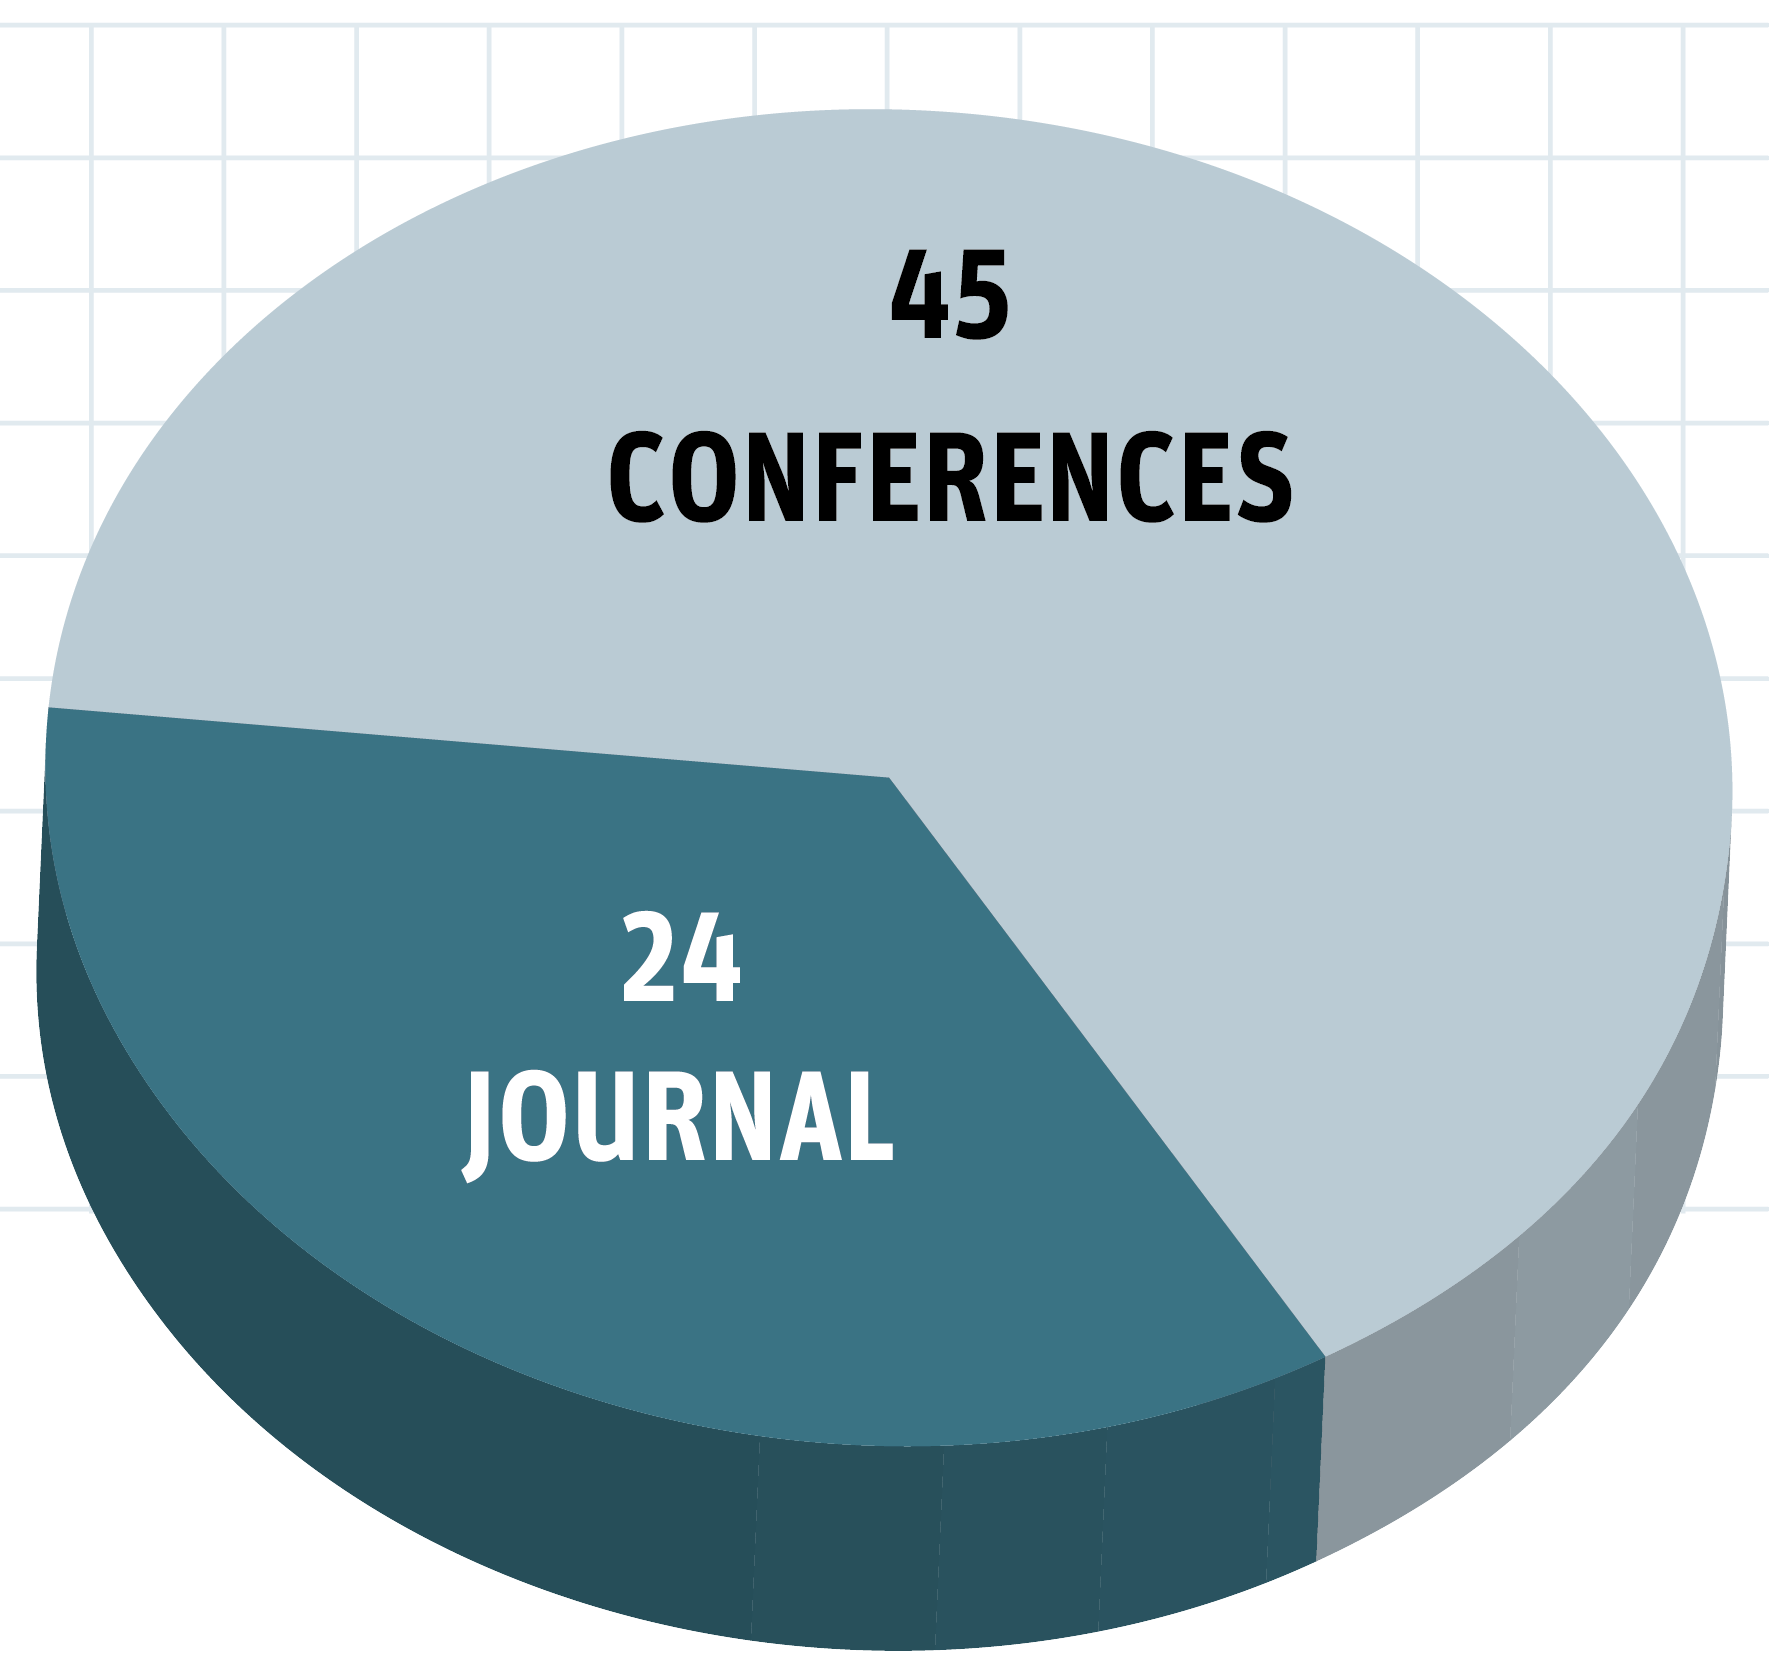
\includegraphics[width=0.92\textwidth, keepaspectratio]{Prancheta 3 (2).png} 
\end{figure}




\begin{table}[!ht]
  \centering
  \captionsetup{
    format=hang,
    justification=raggedright,
    singlelinecheck=false,
    skip=9pt,
  }
  \caption{\MakeUppercase{Venues with higher number papers}}
  \label{table:venue}
  \def\arraystretch{1.2} 
  \begin{tabularx}{\textwidth}{>{\raggedright\arraybackslash}p{4cm}>{\centering\arraybackslash}cX}
    \arrayrulecolor{white}
    \rowcolor{white}
    \textbf{Venue} & \textbf{Total} & \textbf{Papers} \\
    \arrayrulecolor{cor_tabela} \hline
    
    IEEE Transactions on Intelligent Transportation Systems & \cellcolor{cor_tabela}4 & \cellcolor{cor_tabela}\cite{Broggi2015a,Tas2018a,Aramrattana2018,Sajjad2020} \\
    \arrayrulecolor{cor_tabela} \hline
    
    IEEE Intelligent Vehicles Symposium & \cellcolor{cor_tabela}3 & \cellcolor{cor_tabela}\cite{Broggi2015,Kunz2015,Kessler2019} \\
    \arrayrulecolor{cor_tabela} \hline
    
    International Interdisciplinary PhD Workshop (IIPhDW) & \cellcolor{cor_tabela}2 & \cellcolor{cor_tabela}\cite{Percinski2018}, \cite{Gotlib2019} \\
    \arrayrulecolor{cor_tabela} \hline

  \end{tabularx}
\end{table}

\color{black}

Furthermore, citation analysis software \cite {vanEck2010} was used to generate a co-citation map. The co-citation analysis, when applied to venues, enables the identification of core journals and conferences in a specific field, highlighting those that significantly influence the development and dissemination of research. It also evaluates the prestige and impact of a publishing venue within the academic community \cite{MINGERS2015}.

\begin{figure*}[ht]
  \centering
  
  % Caption setup for this specific figure
  \captionsetup{
     labelsep=newline,
     labelfont={bf,large},       % label (e.g., "Figure 1:") in bold and large
     textfont={bf,large},        % caption text in bold and large
     justification=centering,  % left-align the caption
     singlelinecheck=off         % force left alignment even for short captions
  }
  
  \caption{\MakeUppercase{Co-citation journals from the ADV prototype papers}}
  \label{fig:Cosources}
  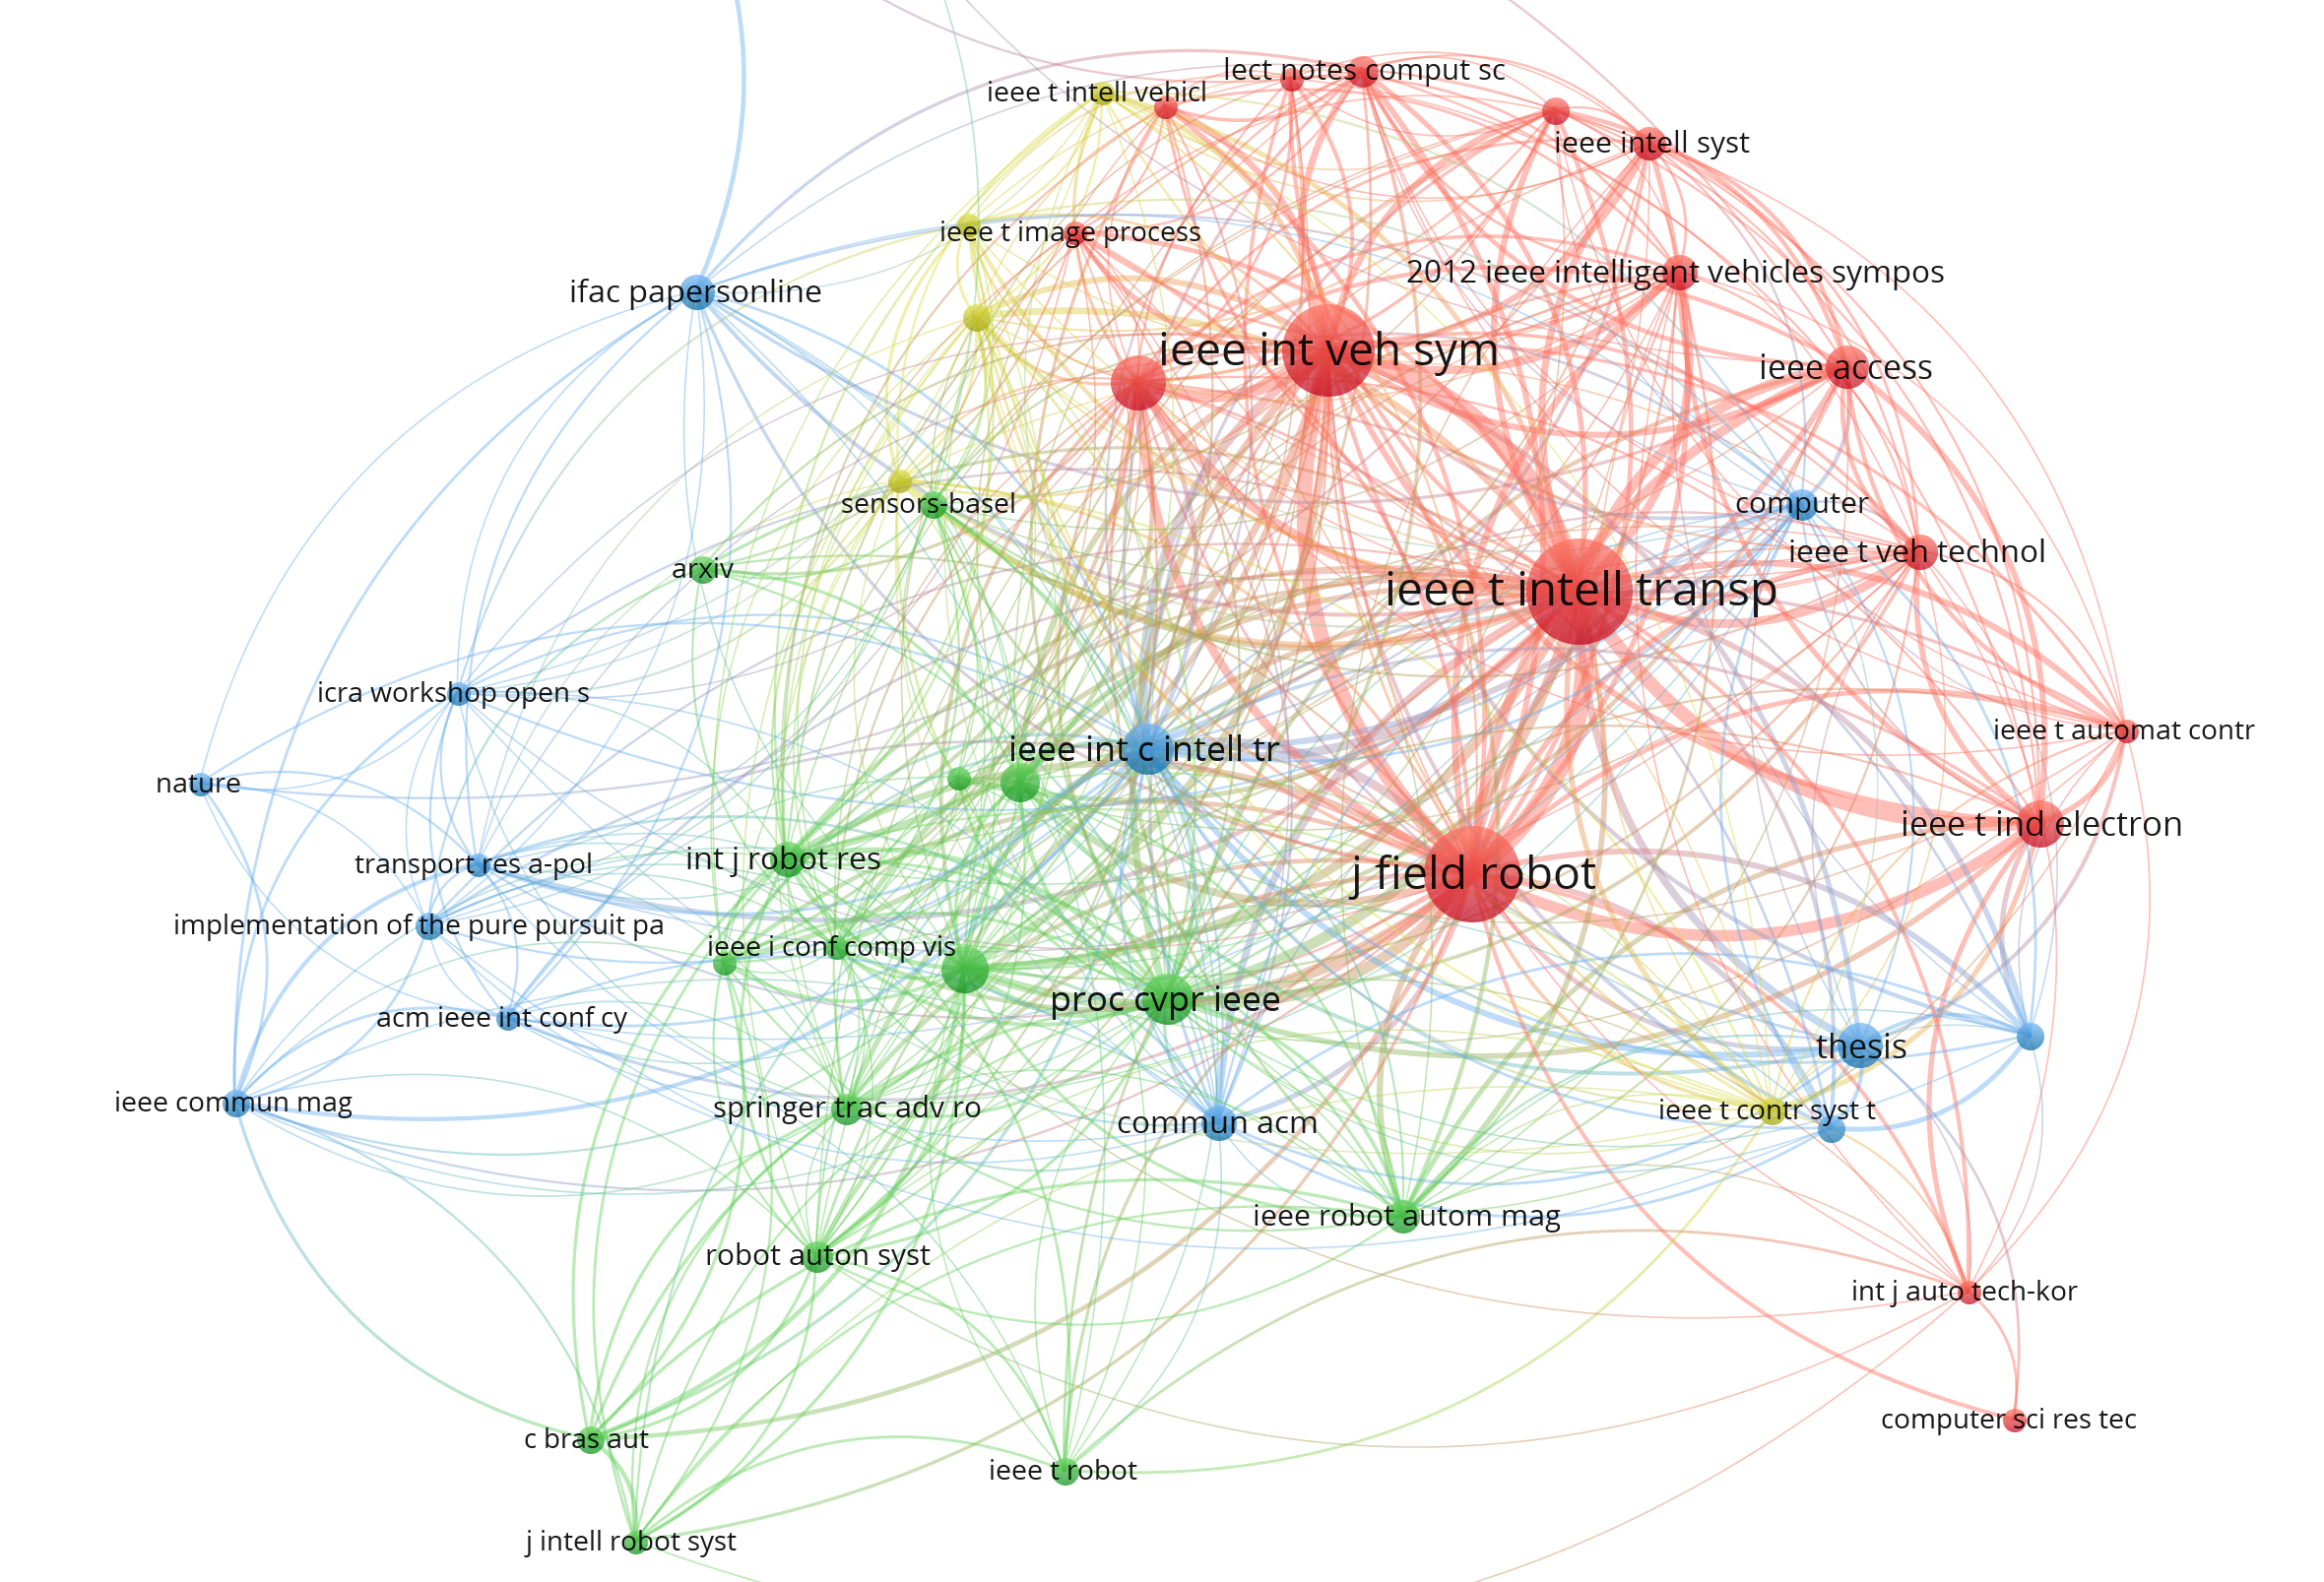
\includegraphics[width=.8\textwidth, keepaspectratio]{CocitationCitedSources.png} 
\end{figure*}

To generate the co-citation map from all references from the analyzed articles, the criteria of a minimum of three citations per journal were used, resulting in 55 publishers being shown in Figure \ref{fig:Cosources}. The map indicated that the IEEE Intelligent Vehicles Symposium conference, the IEEE Transactions on Intelligent Transportation Systems, and the Journal of Field Robotics journals are the most influential group of publishing venues, leading the red cluster and influencing all small clusters around them. Interestingly, the Journal of Field Robotics has a strong influence as the venue where one of the main articles of the field was published \cite{Urmson2008}, although none of the prototypes analyzed came from there.

\color{black}



\subsection*{\textbf{PQ2  How is the publication distribution per year?}}

Figure \ref{fig:year} shows the total number of publications per year. The number of publications decreased in 2016 and 2017, which could be the time necessary to adopt the changes in machine learning and processing power that happened up to 2015.

This also occurred in 2021 and 2022. In these two years, we found many papers about improvements in algorithms and technologies for autonomous vehicles. (e.g., artificial intelligence, computer vision, path planning, architectures, sensors). Therefore, the low number of publications on prototypes in 2021 and 2022 can be explained by the fact that, in this period, there was more research focused on improving technologies for autonomous driving vehicles because the publications in 2018, 2019, and 2020 proposed many contributions related to prototypes. 

\begin{figure}[ht]
  \centering
  
  % Caption setup for this specific figure
  \captionsetup{
     labelfont={bf,large},       % label (e.g., "Figure 1:") in bold and large
     textfont={bf,large},        % caption text in bold and large
     justification=raggedright,  % left-align the caption
     singlelinecheck=off         % force left alignment even for short captions
  }
  
  \caption{\MakeUppercase{Publications distribution per year}}
  \label{fig:year}
  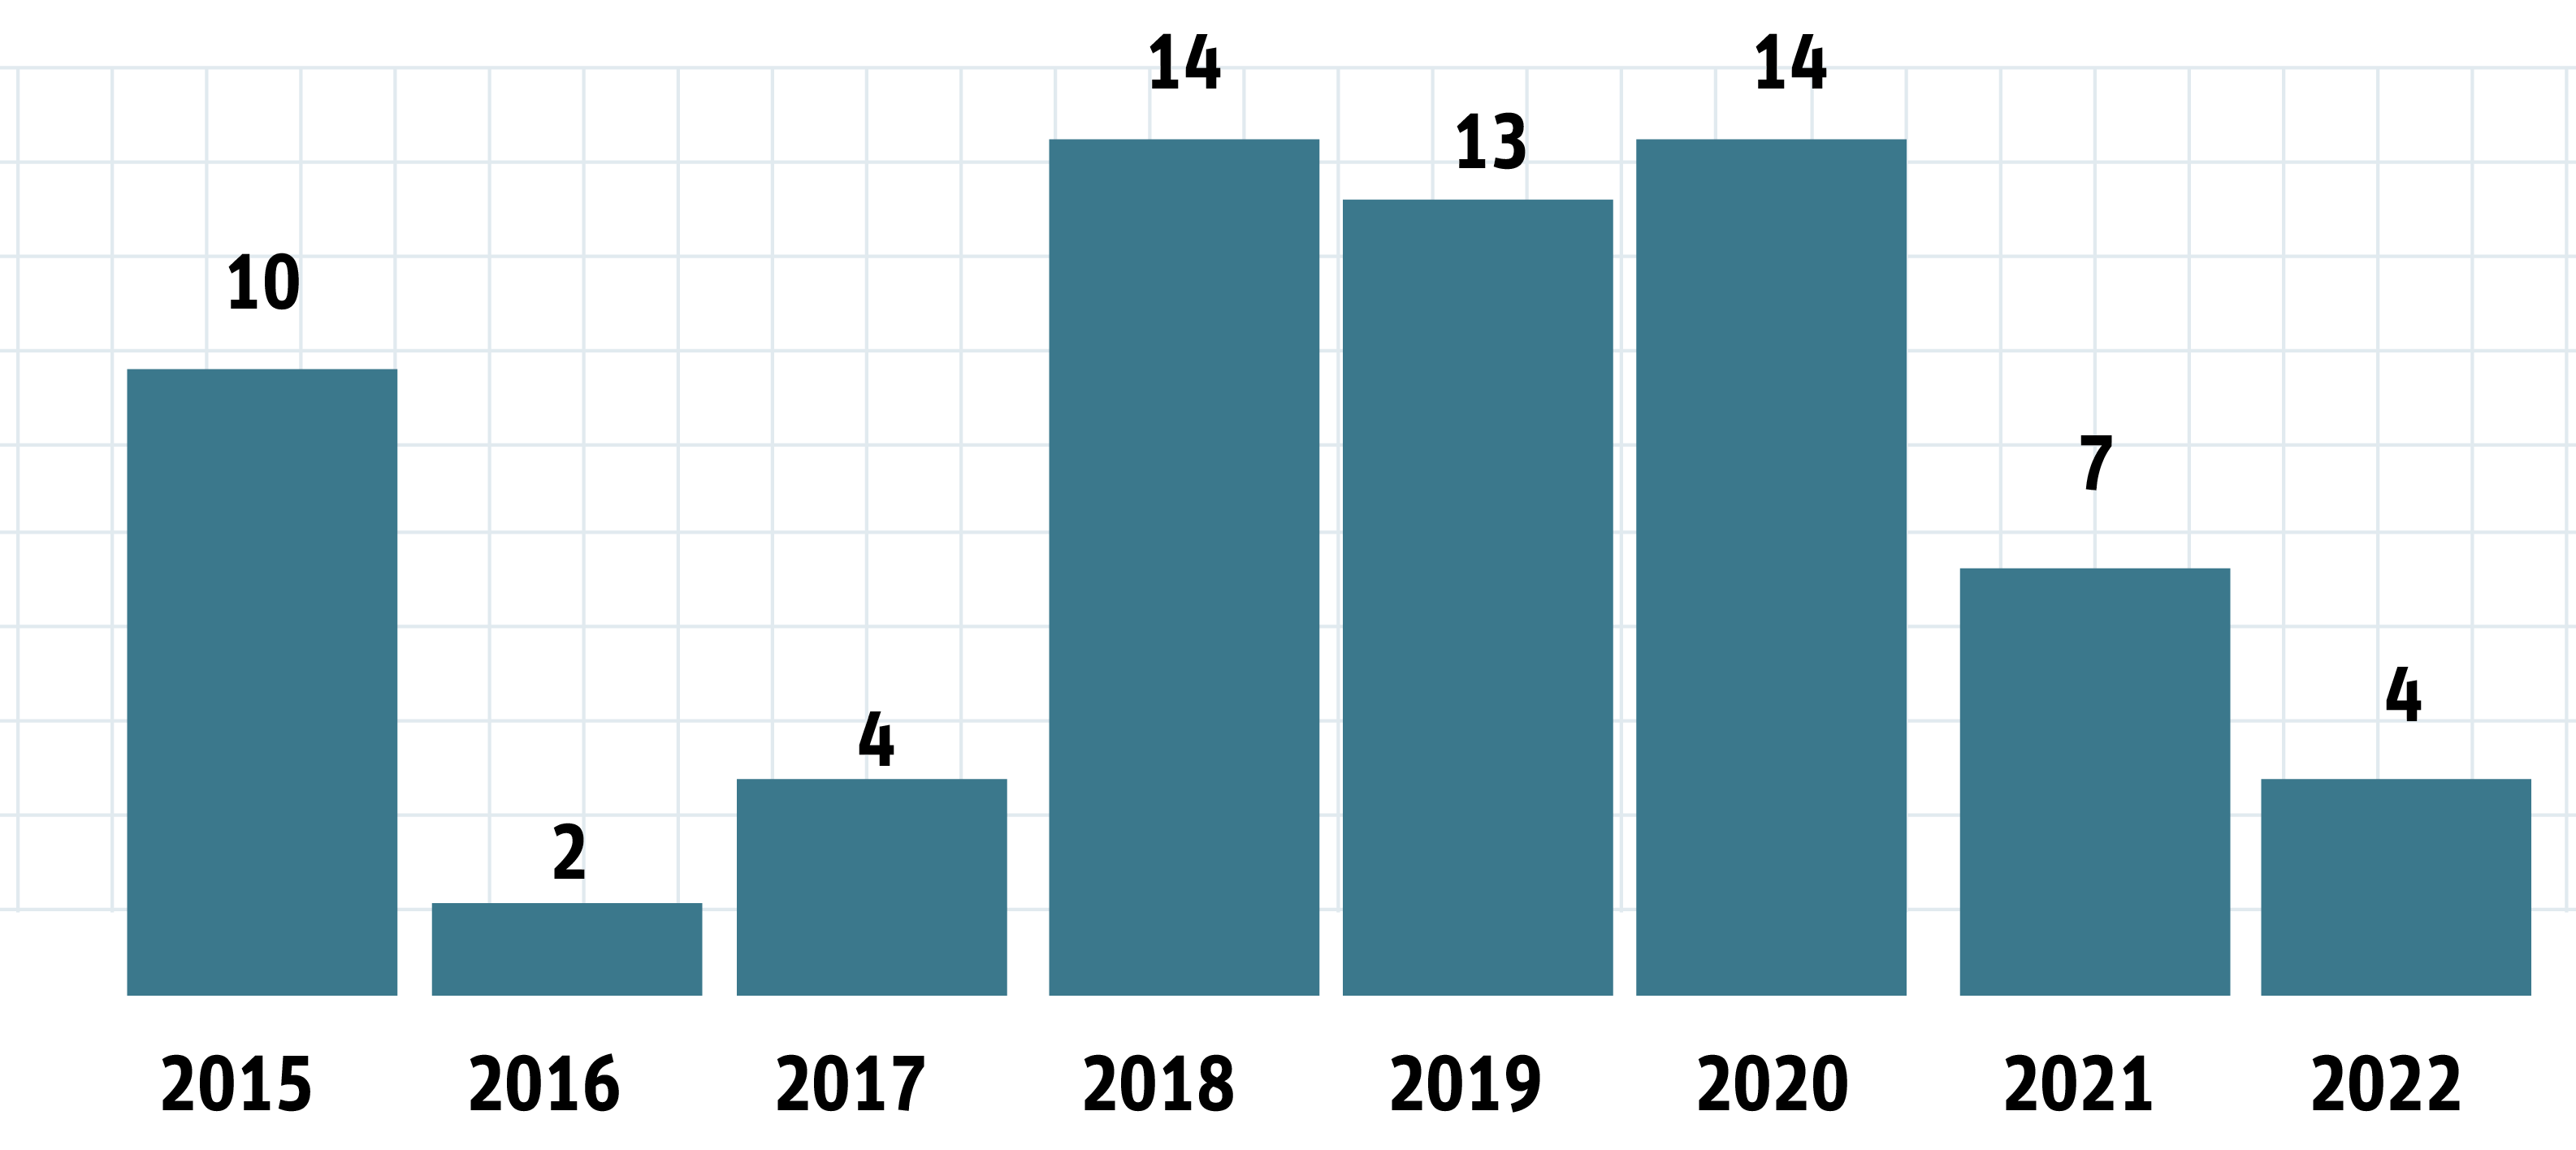
\includegraphics[width=\textwidth, keepaspectratio]{Prancheta 4 (2).png} 
\end{figure}


\subsection*{\textbf{PQ3  What is the researchers' affiliation?}}

We aim to identify if ADV development was most concentrated in academia, industry, or research centers. All the selected papers from mini prototypes were developed in academia. In the commercial vehicles prototypes it was found two papers that were a collaboration between academia and industry \cite{Buechel2015} \cite{buchegger2018}, three papers published by industry research teams \cite{Gupta2015,Bojarski2016,Belcarz2018} and one published by a research center \cite{Tas2018}. 

It does not mean that industry is not interested in ADV development, but rather that the information is not being disclosed in academic papers due to the intense competition between the companies aiming to be the ones to lead the autonomous vehicle market. Many companies advertise their ADV solutions, as mentioned in the previous sections. However, they must clarify the proposed solution with a few exceptions, such as the Apollo Company \cite{Apollo}.

\subsection*{\textbf{PQ4  What are the most active publishing countries}}

\color{black}
By applying the analysis software and using the information collected from the SCOPUS database, it could be possible to identify the most prolific countries and their number of citations in the development of ADV. The ADV papers used in this study have shown that researchers from 35 countries have developed an ADV prototype. Figure \ref{fig:country} shows the distribution of the leading countries. This graph considers the countries with more than one paper published according to this mapping study. Additionally, we generate the Table \ref{table:qtd_citacoes} to verify the depth of the influence of the publications from each country. 
 
\begin{figure}[ht]
  \centering
  
  % Caption setup for this specific figure
  \captionsetup{
     labelfont={bf,large},       % label (e.g., "Figure 1:") in bold and large
     textfont={bf,large},        % caption text in bold and large
     justification=raggedright,  % left-align the caption
     singlelinecheck=off         % force left alignment even for short captions
  }
  
  \caption{\MakeUppercase{Most active countries}}
  \label{fig:country}
  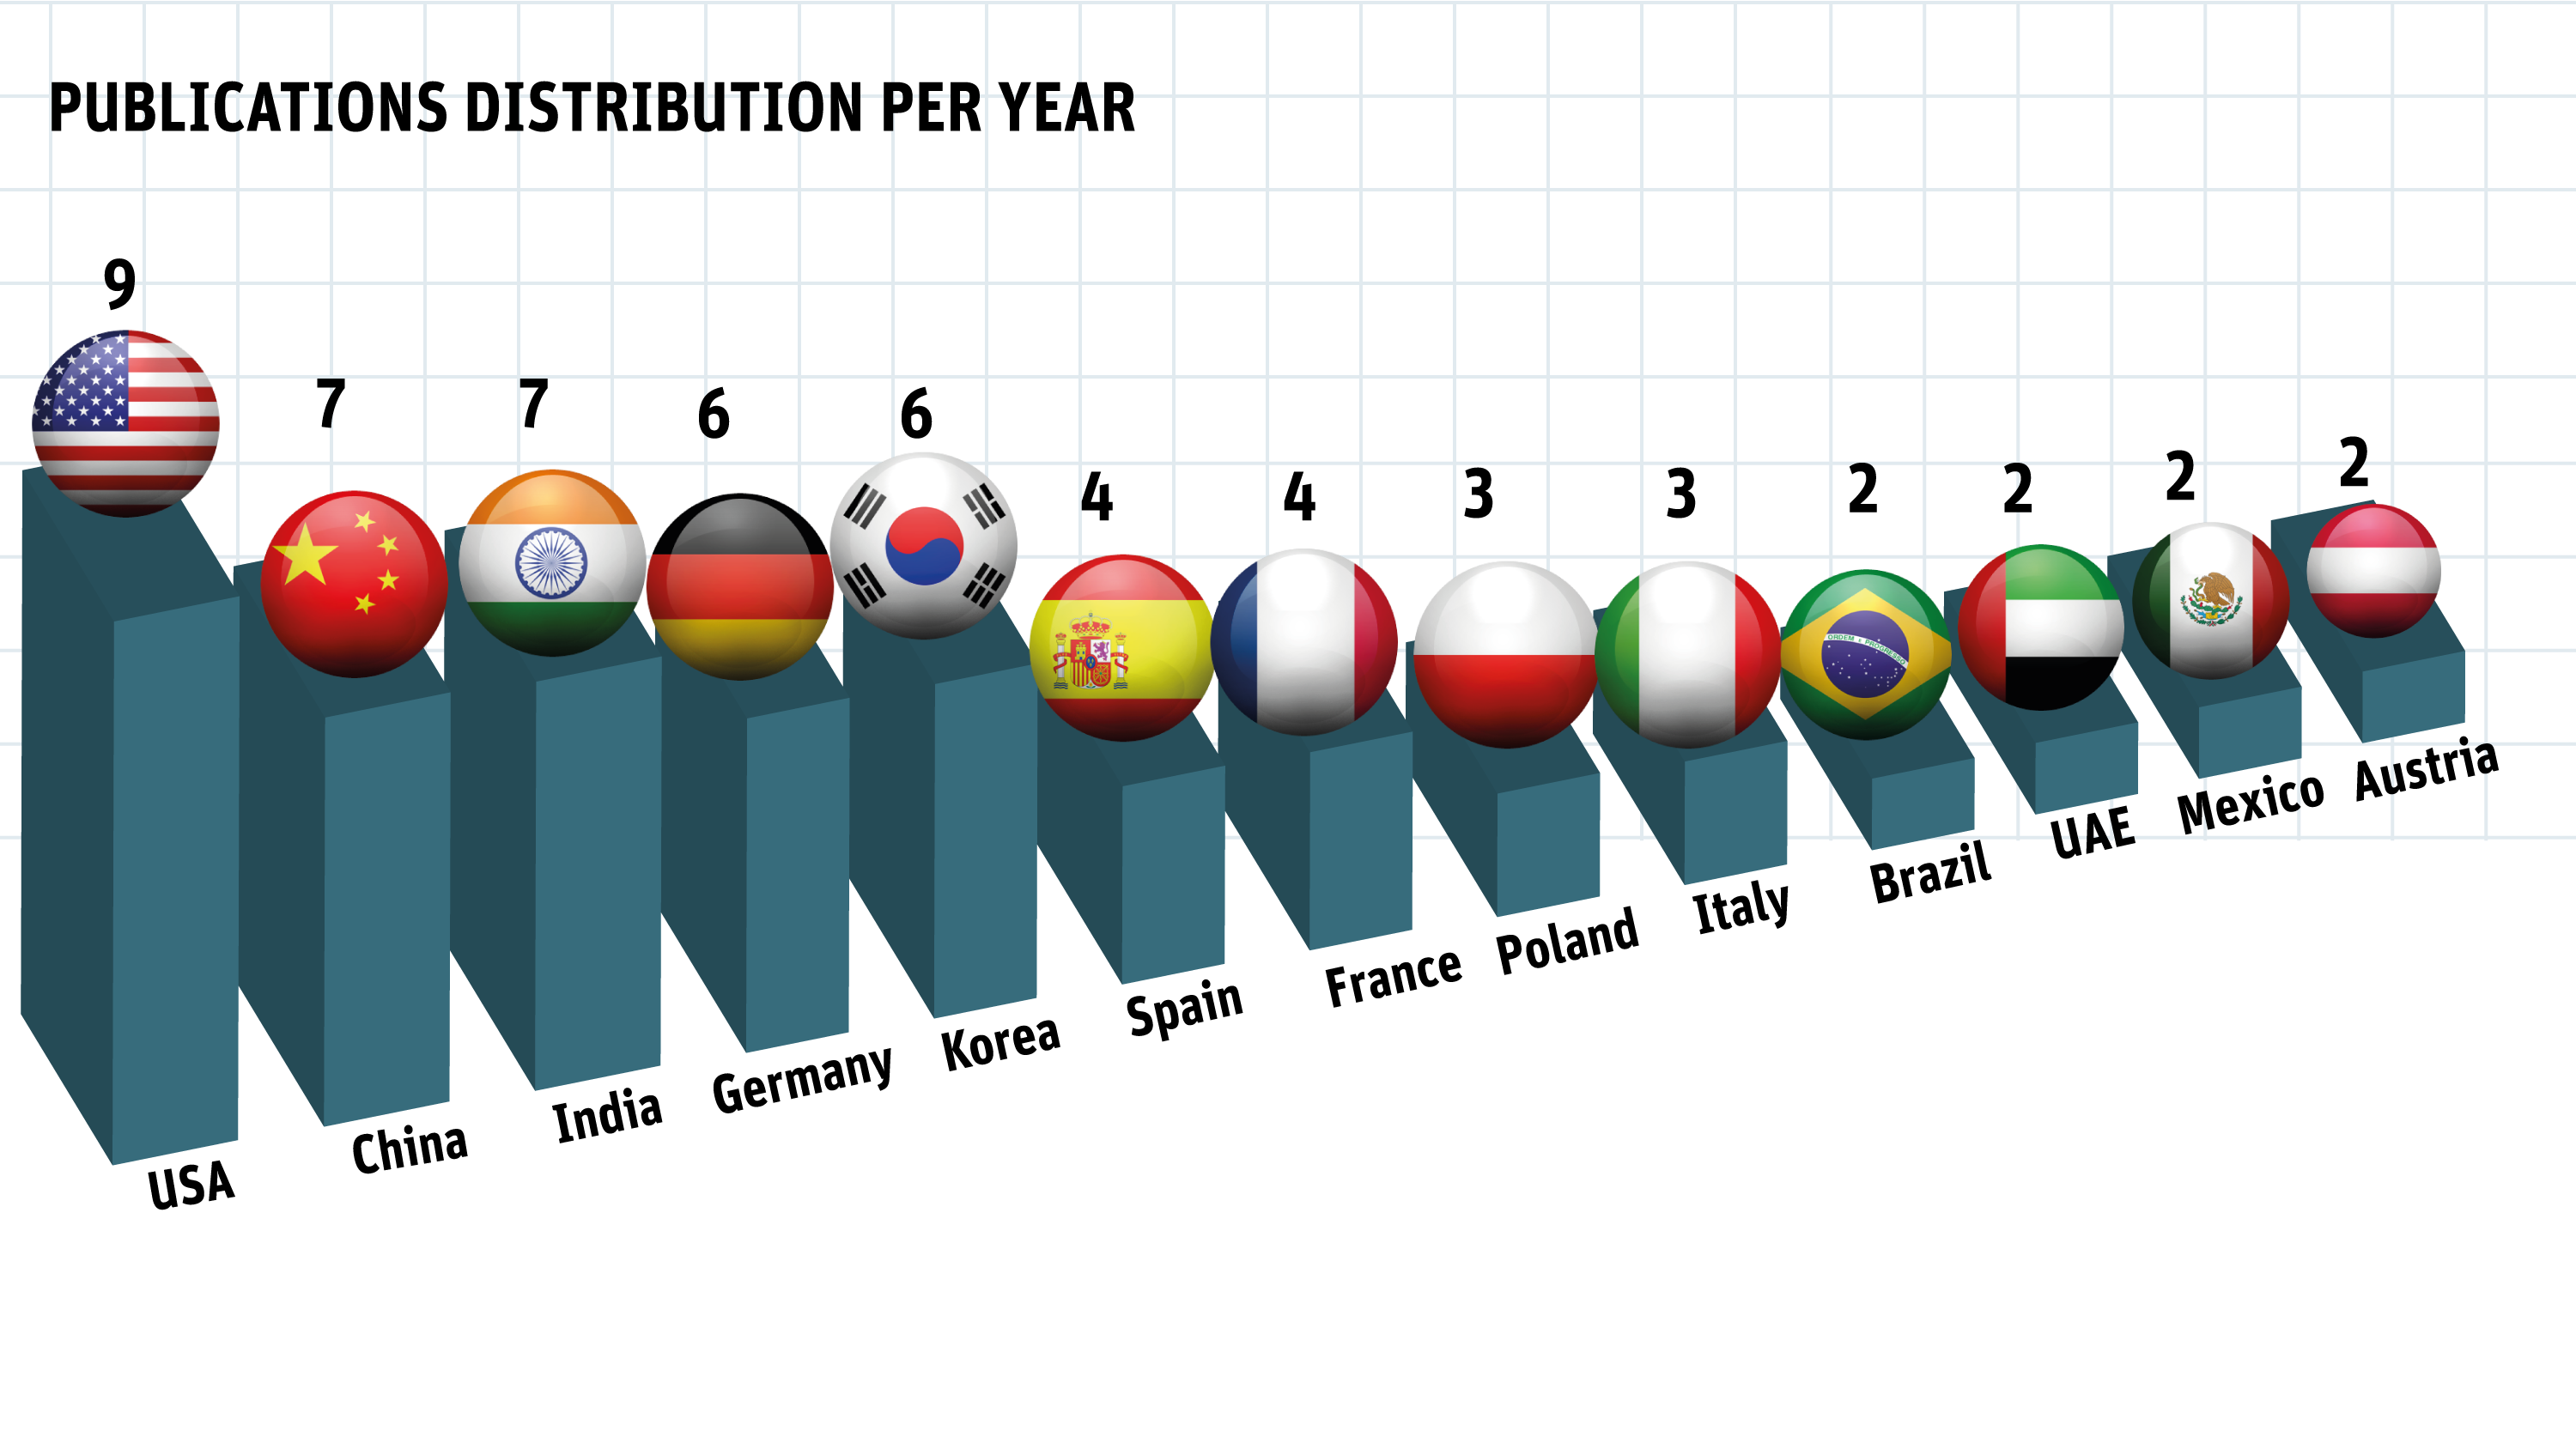
\includegraphics[width=\textwidth, keepaspectratio]{Prancheta 2 (2).png} 
\end{figure}


\color{black}
\begin{table}[!ht]
  \centering
  \captionsetup{
    format=hang, % Add this line to create hanging indent for the caption
    justification=raggedright,
    singlelinecheck=false,
    skip=9pt, % Adjust the distance between caption and table
  }
  \caption{\textcolor{black}{\MakeUppercase{Number of Total Citations per Country}}}
  \label{table:qtd_citacoes}
  \def\arraystretch{1.5}
  \begin{tabularx}{\textwidth}{>{\centering\arraybackslash}X>{\centering\arraybackslash}X}
    \arrayrulecolor{white}
    \rowcolor{white}
    \textbf{\textcolor{black}{Country}} & \textbf{\textcolor{black}{Quantity of Citations}} \\
    \arrayrulecolor{cor_tabela} \hline
    \textcolor{black}{Germany} & \cellcolor{cor_tabela}\textcolor{black}{938} \\
    \arrayrulecolor{cor_tabela} \hline
    \textcolor{black}{Japan} & \cellcolor{cor_tabela}\textcolor{black}{395} \\
    \arrayrulecolor{cor_tabela} \hline
    \textcolor{black}{South Korea} & \cellcolor{cor_tabela}\textcolor{black}{370} \\
    \arrayrulecolor{cor_tabela} \hline
    \textcolor{black}{Italy} & \cellcolor{cor_tabela}\textcolor{black}{244} \\
    \arrayrulecolor{cor_tabela} \hline
    \textcolor{black}{United States} & \cellcolor{cor_tabela}\textcolor{black}{189} \\
    \arrayrulecolor{cor_tabela} \hline
    \textcolor{black}{China} & \cellcolor{cor_tabela}\textcolor{black}{111} \\
    \arrayrulecolor{cor_tabela} \hline
    \textcolor{black}{Vietnam} & \cellcolor{cor_tabela}\textcolor{black}{74} \\
    \arrayrulecolor{cor_tabela} \hline
    \textcolor{black}{Brazil} & \cellcolor{cor_tabela}\textcolor{black}{72} \\
    \arrayrulecolor{cor_tabela} \hline
    \textcolor{black}{India} & \cellcolor{cor_tabela}\textcolor{black}{64} \\
    \arrayrulecolor{cor_tabela} \hline
    \textcolor{black}{France} & \cellcolor{cor_tabela}\textcolor{black}{40} \\
    \arrayrulecolor{cor_tabela} \hline
    \textcolor{black}{Spain} & \cellcolor{cor_tabela}\textcolor{black}{32} \\
    \arrayrulecolor{cor_tabela} \hline
  \end{tabularx}
\end{table}

\color{black}
It is interesting to see that the United States and China, being the top two in the number of publications, having nine and seven papers on ADV prototypes, are only in fifth and sixth place, with much fewer citations than the top three countries in the number of citations, showing a lack of impact of their publications in the research community. On the other hand, Germany shows a strong influence from their publications, having the most citations, much more than the second and third-place countries, Japan and South Korea. Japan is an interesting case, as only one ADV prototyping paper has been published. However, it was a breakthrough paper \cite{Kato2015} that developed the Autoware \cite{Autoware}, a software stack framework based on ROS \cite{ros} that was largely adopted by the research community, being the first open-source software developed for autonomous driving functionalities.





\color{black}
\subsection*{\textbf{PQ5  What are the leading references?}}

The published results of breakthroughs could influence the entire field of research, which is basically what happened in the ADV prototype development field. Applying co-citation mapping in references, these trend-creator papers could be easily found \cite{MINGERS2015}. From the 68 prototype papers, we have applied the co-citation analysis software, setting it up only to use the references cited at least twice to remove non-relevant references and make the network cleaner to Explorer. This left 59 references to be processed by the software.

\begin{figure*}[ht]
  \centering
  
  % Caption setup for this specific figure
  \captionsetup{
     labelfont={bf,large},       % label (e.g., "Figure 1:") in bold and large
     textfont={bf,large},        % caption text in bold and large
     justification=raggedright,  % left-align the caption
     singlelinecheck=off         % force left alignment even for short captions
  }
  
  \caption{\MakeUppercase{Co-citation reference from the ADV prototype papers}}
  \label{fig:Coref}
  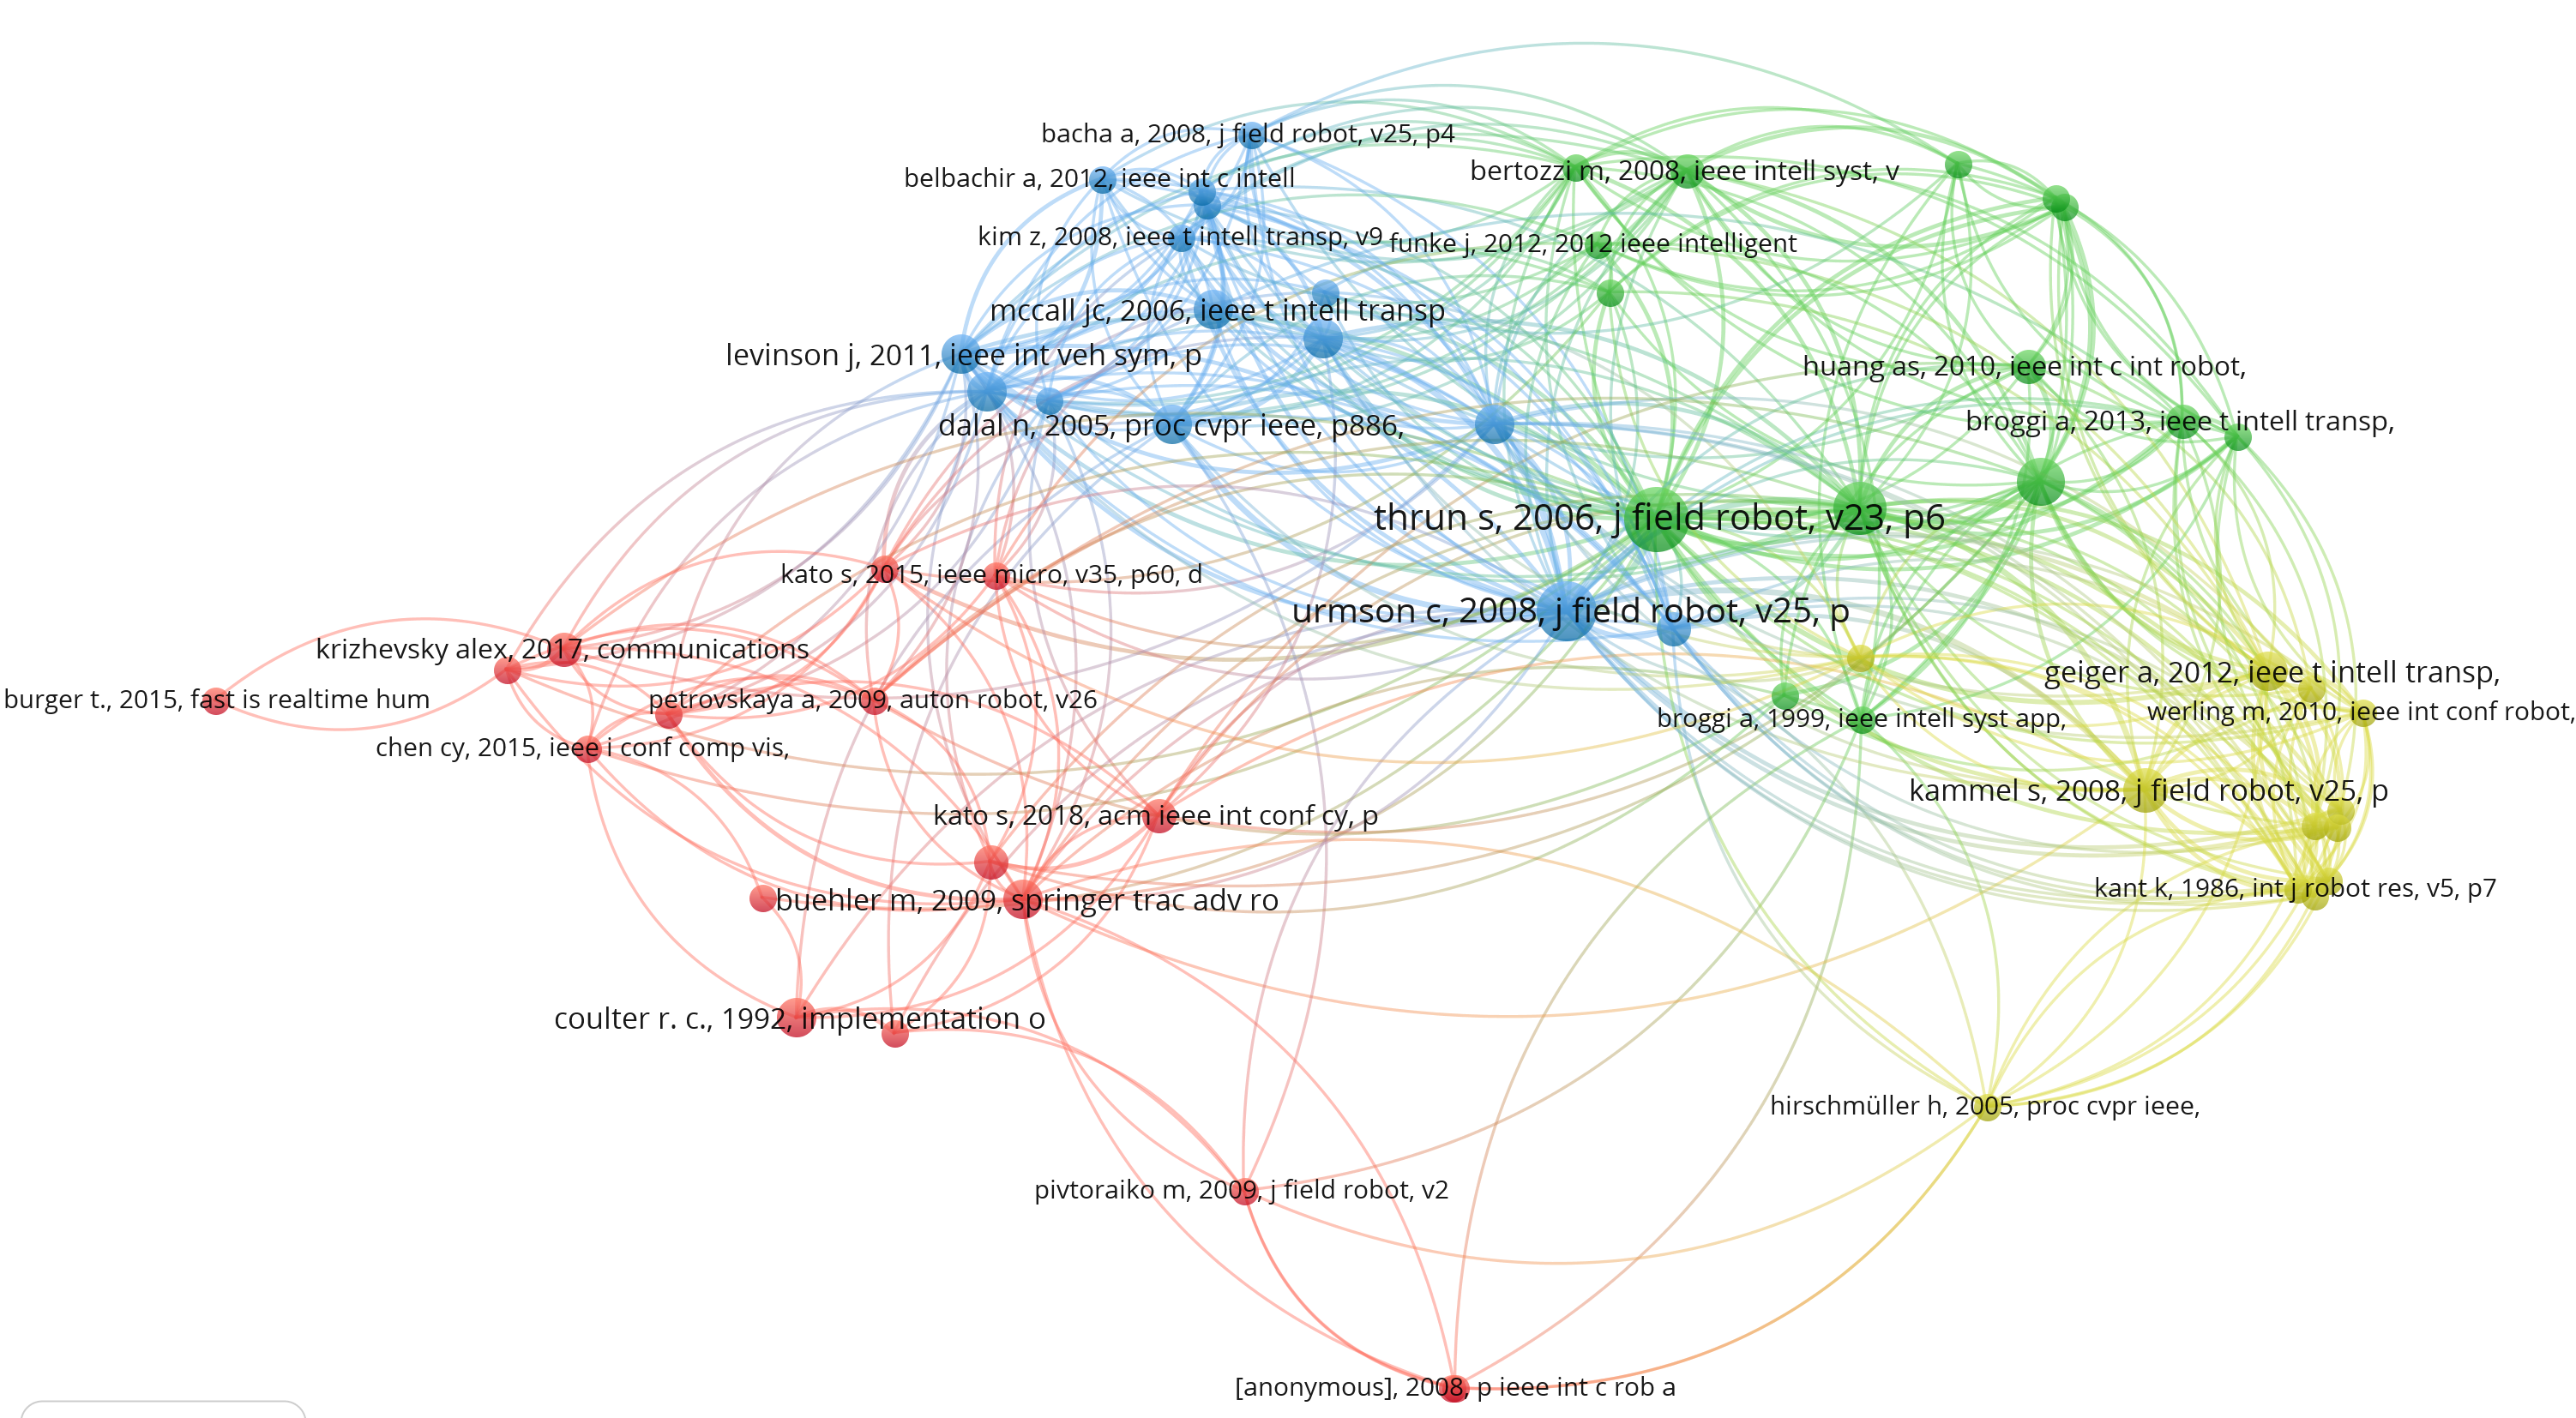
\includegraphics[width=\textwidth, keepaspectratio]{ReferencesCocitationMin2.png} 
\end{figure*}

The results shown in Figure \ref{fig:Coref} present four different clusters of reference nodes in the colors red, blue, yellow, and purple. The ones with strong citations, among other papers in the field, are represented by the bigger nodes that influence all the other researchers in the field. Looking at the main nodes of each cluster \cite{Urmson2008,Thrun2006,Buehler2009,Kammel2008}, it could be concluded that the incentive of the Darpa Challenges \cite{Darpa} from 2004 up to the recent days, but especially 2006, 2008, and 2009 competitions, by offering prestige and a million us dollars money prize, was pivotal for the development of the ADV prototyping technology as we see today. Furthermore, the Grand Cooperative Driving Challenge (GCDC) \cite{GCDC}, a competition between European universities, helped to boost the development of ADV by having a prototyping team that participates in both competitions \cite{Geiger2012}. The co-citation analysis also clarifies why the Journal of Field Robotics was so influential in the prototyping field as almost every participant of the Darpa challenge published its prototype research paper in it \cite{Leonard2008, Bacha2008,Montemerlo2008, Thrun2006,Kammel2008,Urmson2008,Urmson2009,Buehler2009}.

The red cluster is an interesting group of references as it brought together some milestone studies in the ADV field, not only related to prototypes but also to the supporting technology necessary to develop them, such as the release of the robot operating system (ROS) \cite{quigley2009}, the winning team for the ImageNet 2012 classification competition \cite{Krizhevsky2017} that made possible a significant advance in image detection and classification technology and the development of the open source software Autoware \cite{Kato2015} for the development of autonomous driving systems and its posterior application \cite{Kato2018}.

Although the main green cluster article is the winner vehicle of the 2006 Darpa challenge \cite{Thrun2006}, this group of publications focused on the deployment and testing of ego and cooperative ADV prototypes, influenced by Alberto Broggi \cite{Broggi1999, Broggi2013, Broggi2015, Broggi2015a} a senior researcher who has been deploying autonomous vehicles for more than 20 years. It shows how a strong researcher can lead a field with continuous publications. The yellow cluster of papers tends to aggregate publications related to ADV perception systems such as \cite{hirschmuller2005, dickmanns1990} and has as its main article the Team AnnieWay vehicle prototype \cite{Kammel2008} that could participate in both Darpa and GCDC competitions.

Furthermore, four participants in the Darpa challenge \cite{Montemerlo2008, Urmson2008, Bacha2008, Leonard2008} are in the blue cluster that heavily influenced the next generation of ADV prototypes \cite{levinson2011, Bertozzi2013, Chu2012, Jo2014}. In addition, the papers in these groups focus on lane detection and path planning strategies applied in the previous group of prototypes. This covers the majority of papers that have driven the development of ADV prototypes nowadays.

\color{black}
\subsection*{\textbf{PQ6  What are the main research topics?}}

The analysis of the co-occurrence of words can reveal the most prevalent concepts within a scientific field, showing changes and stability in topics over time. It can highlight persistent themes, those that fade, and new topics that emerge, often in response to technological developments. This analysis helps establish research priorities and academic planning \cite{Sedighi2016}.
 
With the help of the reference analysis software, excluding the keywords that appeared only once, 71 keywords were found that, after mapping, formed seven clusters, four of which are the main ones with relevant information. This can be seen in Figure \ref{fig:Cokey}. It shows a division between the hot topics studied by the community.


\begin{figure*}[ht]
  \centering
  
  % Caption setup for this specific figure
  \captionsetup{
     labelfont={bf,large},       % label (e.g., "Figure 1:") in bold and large
     textfont={bf,large},        % caption text in bold and large
     justification=raggedright,  % left-align the caption
     singlelinecheck=off         % force left alignment even for short captions
  }
  
  \caption{\MakeUppercase{Co-ocurrence keywords from the ADV prototype papers}}
  \label{fig:Cokey}
  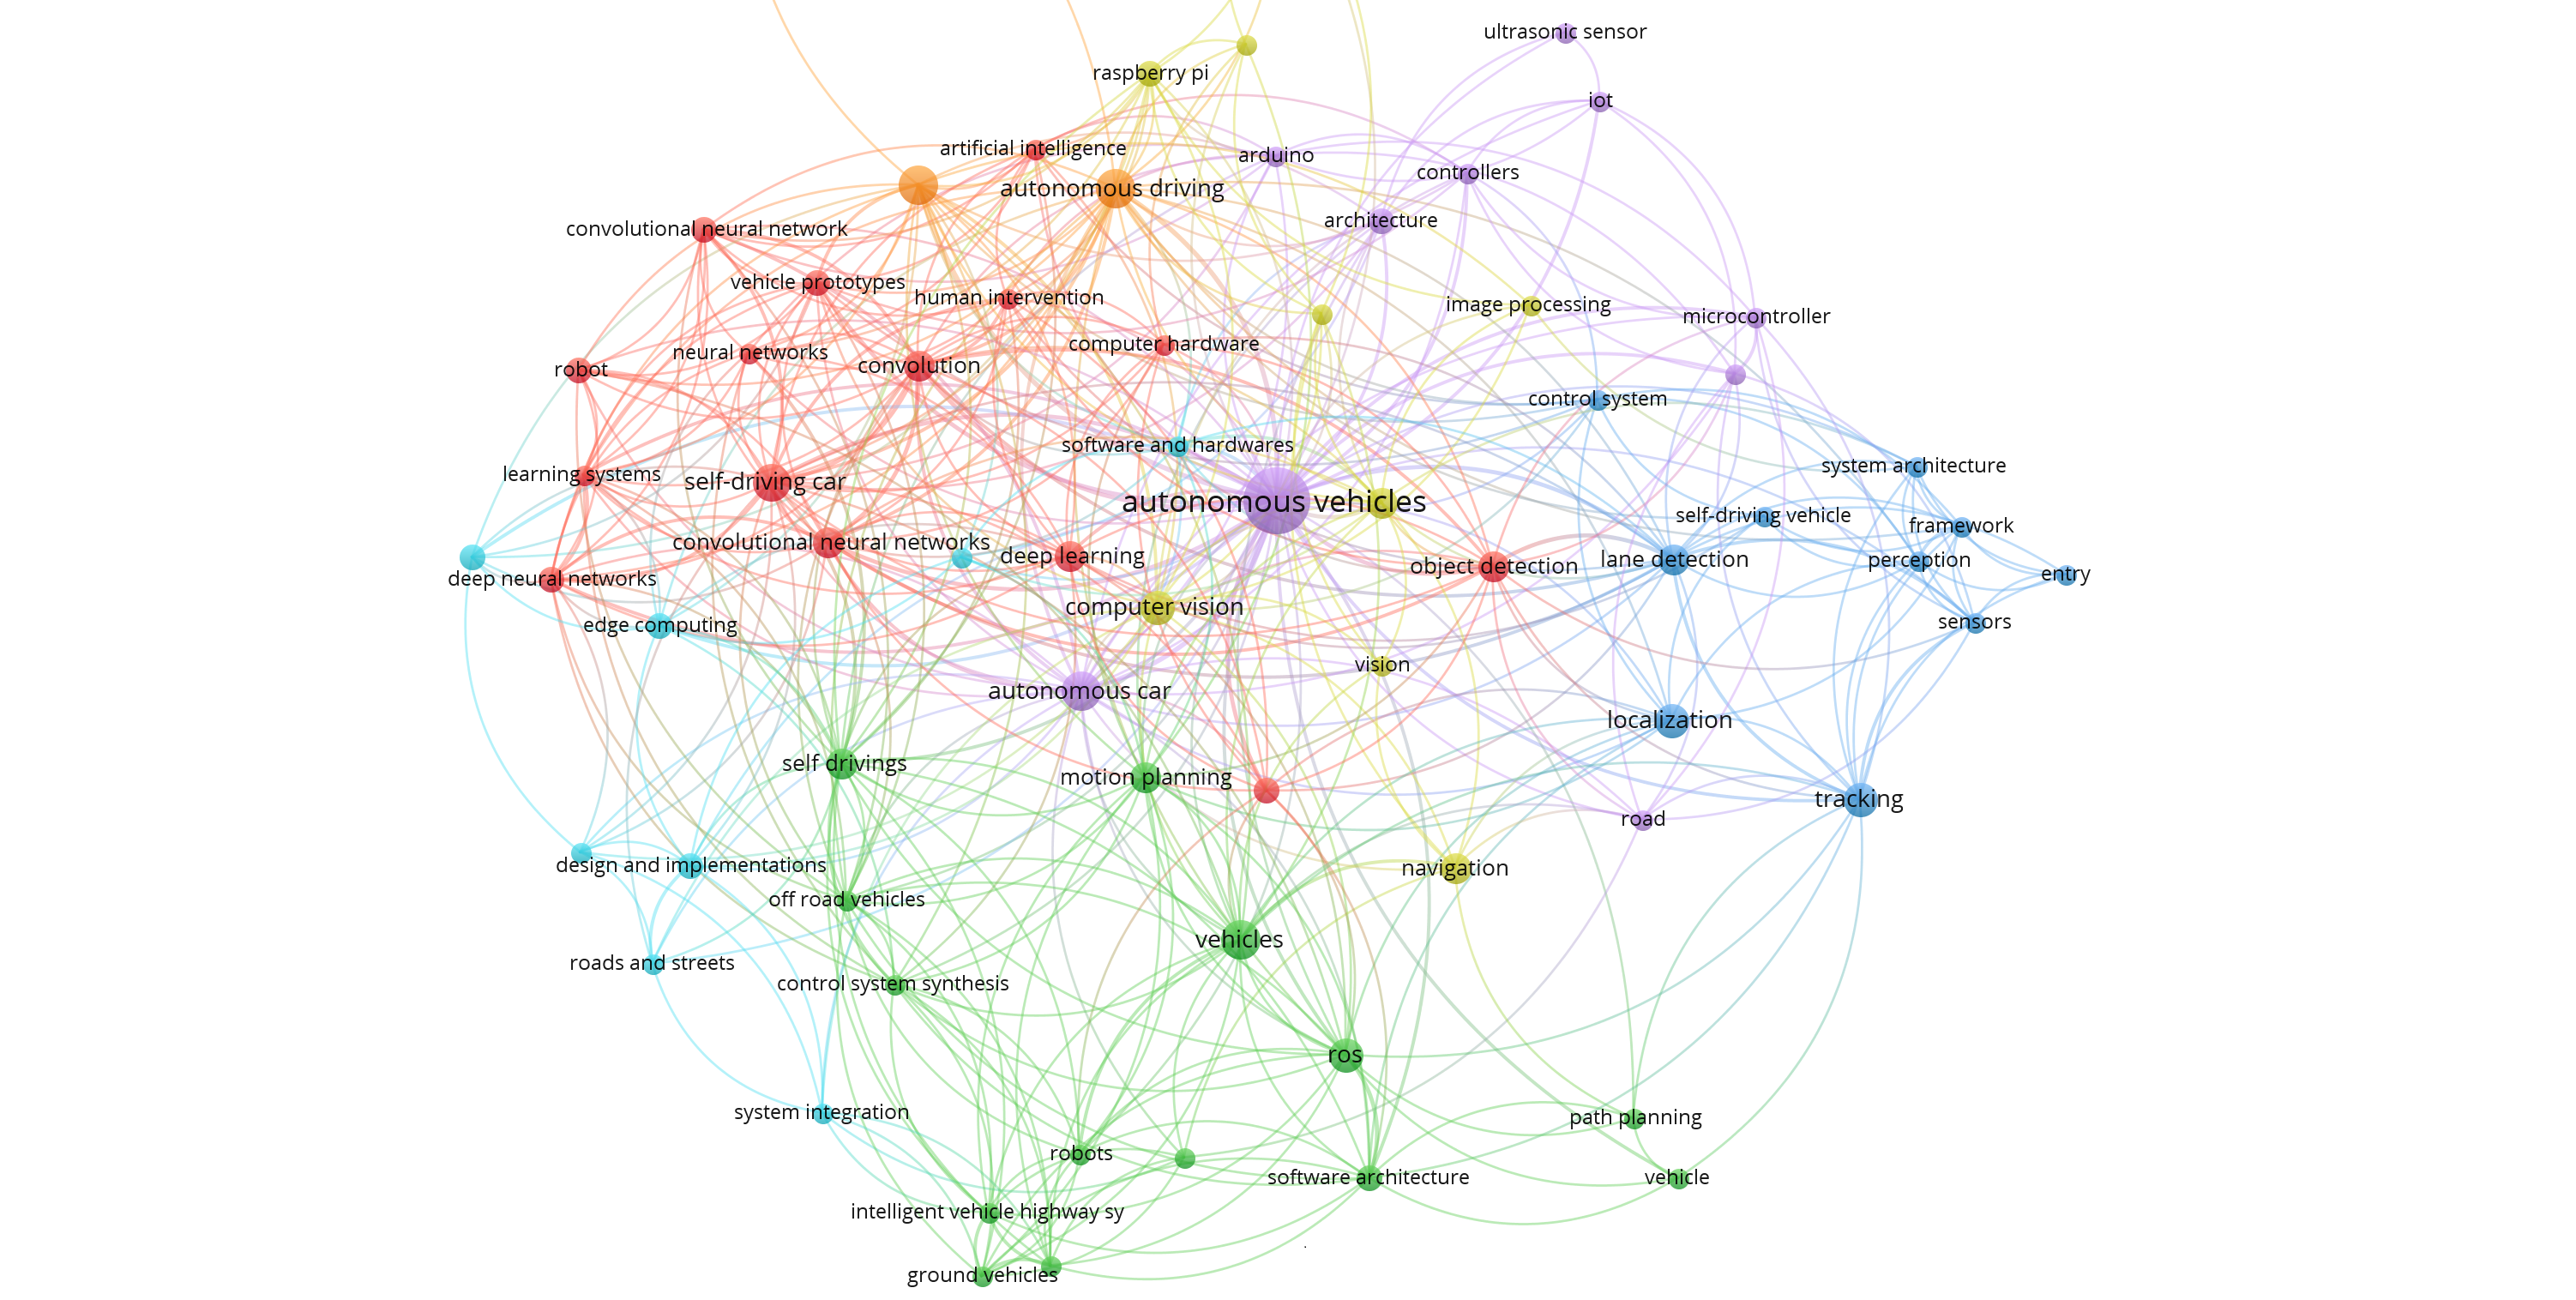
\includegraphics[width=\textwidth, keepaspectratio]{keywordsCORCI2min.png} 
\end{figure*}

The main nodes are the keywords that describe autonomous vehicles and their synonyms. The blue cluster brings the keywords related to the prototype perception system. Lane detection, localization, and tracking are the most recurrent research topics among research works. On the other hand, the red cluster brings the application of neural networks as a hot topic in the ADV prototyping field. It shows vehicle prototypes as a keyword closely connected to convolutional neural networks and their synonyms and deep learning, showing that these are fundamental concepts for developing a prototype.

The green cluster contains the ROS node, which, by its connection, suggests that it should be closely related to developing a software architecture applicable to motion and path planning. The purple node shows the keywords for developing a mini prototype, as devices like the Arduino microcontroller are heavily applied to ADV concept testing with ultrasonic sensors. Image processing for computer vision applied to navigation is also a popular topic in the yellow cluster. In conclusion, all aspects of the perception system, such as lane detection, object detection and localization, image processing, deep learning, and the planning systems of the vehicle, are still hot topics among researchers.

\color{black}
\section{Open Research Issues}

Several vehicle prototypes can show us a trend. However, they also can lead to different choices of hardware, software, and sensors for ADV were found in many domains, providing an enormous opportunity for discovery and exploration. Our mapping shows that there are open issues and opportunities to research. This section discusses some important research fields about developing prototypes and ADV architectures.

\subsection{5G Network}
The emergence of new 5G networks in recent years has opened up new possibilities for developing autonomous vehicles. There are issues related to speed and quality in the data exchange between the different vehicles.

The newly commercialized 5G network is expected to provide one-millisecond latency, ensuring a reliability of 99.999\%, availability of 99.999\%, and very high throughput of 10 Gbps \cite{10.1145/3485767}. Because it is a new technology, much research related to ADV still needs to present this technology among those used. However, it is a fact that it will collaborate with the future of large and small autonomous vehicles. Therefore, it is important to assess the impact of its use and compare it with other technologies.

\subsection{Robot Operating System 2 (ROS2)}
Several studies used the Robot Operating System (ROS) software for developing ADV prototypes (small or large prototypes)
\cite{Gupta2015,Martin2016,Tas2018a,Munir2018,Belcarz2018,Betz2019,Marin-Plaza2019,valera2019design,Reke2020,Angel2020,el2020,Karaman2017,al2018,Gotlib2019,Zhou2019,Wang2019,ILIE2020530,app11167225,10.1145/3556548.3559631}. This software is an open-source framework developed for robotic applications, such as ADV, offering libraries and communication layers. Other surveys also chose other frameworks, for instance, Apollo \cite{Kessler2019} \cite{Buyval2019}, and Autoware \cite{el2020autonomous}. Both frameworks are also extended versions of ROS.

ROS has been evolving into ROS2, a second version that maintains the modularity of the first version and has real-time performance improvements \cite{Reke2020}. Furthermore, according to the ROS and ROS2 website \cite{ros}, ROS2 provides several quality-of-service policies that improve communication on different networks and deliver better features more efficiently at runtime. As a result, more research can use this updated framework version to propose Autonomous Driving Vehicles (ADV) prototypes. Besides, it is important to compare the impacts of its use with previous versions.


\subsection{Simultaneous Localization and Mapping (SLAM)}
Simultaneous Localization and Mapping (SLAM) is the technique used to enable vehicles to move independently. For this, autonomous vehicles need to build maps of the environment while moving and locating themselves. One of the most used sensors for perception, localization, and mapping is the LiDAR (Light Detection and Ranging) \cite{Kessler2019}. Many studies used LiDAR to assist in the SLAM task \cite{Gupta2015,Kato2015,Broggi2015a,Broggi2015,Buechel2015,Belbachir2017,Zong2018,Tas2018a,Munir2018,Belcarz2018,Xu2018,buchegger2018,Kessler2019,Betz2019,Marin-Plaza2019,valera2019design,Angel2020,el2020,Karaman2017,aguilar2017,Percinski2018,fayjie2018,Wang2019,Gotlib2019,Zhou2019,Buyval2019,ILIE2020530,ORJUELA202015161,app11167225,10.1145/3556548.3559631,electronics10192447}. However, that sensor is the barrier to popularizing the ADV due to its high cost, which can get up to 75,000 dollars \cite{Lin2018}. That makes prototype developers search for alternatives for that sensor, like using only cameras \cite{Tang2018}, also used in various surveys \cite{Jo2015,Kunz2015,Kato2015,Broggi2015a,Broggi2015,Buechel2015,Bojarski2016,Belbachir2017,Zong2018,Tas2018a,Munir2018,Belcarz2018,Kessler2019,Betz2019,Marin-Plaza2019,valera2019design,Reke2020,Angel2020,pannu2015,Karaman2017,Bechtel2019,Percinski2018,fayjie2018,deac2018,jain2018,do2018,kwon2018,Sahu2019,Zhou2019,Sun2019,Wang2019,roestam2019,Sajjad2020,Febbo2020,Fathy2020,el2020,chaitra2020,pehlivan2020,Buyval2019,ILIE2020530,ORJUELA202015161,10007388,9297973,albin2021design,app11167225,10.1145/3556548.3559631,9690543,electronics10192447}. Thus, given this scenario, research needs to explore sensor alternatives to replace LiDAR or alternative algorithms for image processing and machine learning that aim to use the images provided by cameras and other sensors to perform the SLAM of the environment.

\subsection{Multi-robots and Edge Computing}
There are many contexts in which multi-robot systems can be used to allow parallel and joint work of different ADV (large and small autonomous vehicles). For instance, in small autonomous vehicles, ground vehicles can work with drones to cover larger areas and different heights.

Multi-robot systems must be able to use Simultaneous Localization and Mapping (SLAM) techniques. Therefore, the localization and mapping of each vehicle are not done independently but in parallel with the other vehicles of the multi-robot operating system in the same environment \cite{9767431}. However, SLAM has a high processing load, and using a efficient cloud system \cite{liu2017b} composed by high-performance edge servers near the vehicles is important. Therefore, an edge server is placed near the vehicle in edge computing to improve responsiveness to many sensor nodes. This results in a concentrated load distribution on the cloud server and eliminates delays and instability caused by network communication \cite{BILAL201894}. In addition to these challenges, no planning algorithm for multiple vehicles considers both global planning and local planning \cite{9902730}.

During the review of the papers, there is still not a considerable number of researchers that explore the context of multi-robot systems. Thus, multi-robot systems are promising opportunities for future research.

\color{black}\subsection{Cybersecurity Concerns} 

Due to its reliance on interconnected systems and components, ADV is susceptible to various cyber threats. Key areas of concern include electronic control units, sensors such as LiDAR and cameras, and the software algorithms that process their data. Cyberattacks can range from altering vehicle operational software to manipulating sensor inputs, compromising safety and functionality \cite{KIM2021}. For example, adversaries could exploit vulnerabilities in the onboard diagnostic port or the vehicle communication system to alter or steal data, disrupt vehicle operations, or gain unauthorized control \cite{PHAM2021}.

To mitigate these threats, there is an urgent need for robust cybersecurity measures specifically designed for the AV environment. This includes developing advanced intrusion detection systems to identify and neutralize threats in real-time and designing vehicle components and communication networks with security in mind \cite{Chattopadhyay2020}. Ensuring the security of ADVs involves not only technological solutions but also a comprehensive approach that includes regulatory frameworks and standards for vehicle manufacturers and software developers. As autonomous driving continues to evolve, so will the cyber threats they face, making ongoing research and development in cybersecurity measures critical for the safe deployment of autonomous vehicles.

\color{black}\subsection{ Level 5 Fully Autonomous Driving}

The advancement of ADV to function reliably in unpredictable weather and road conditions, which is level 5 automation \cite{SAE}, still needs to be achieved but could be met with significant innovations in sensor technology and AI-based adaptive systems. Innovations in LiDAR technology, such as solid-state and Frequency Modulated Continuous Wave (FMCW) LiDAR \cite{kim2022}, offer new possibilities for enhanced detection capabilities in challenging environments. FMCW LiDAR, for instance, is notable for its more extended detection range and immunity to solar light interference, promising substantial improvements in ADVs' ability to navigate adverse weather conditions. Furthermore, incorporating novel sensors, such as stereo thermal and event cameras, into ADVs aims to improve perception in low light conditions and motion robustness, showcasing a potential leap in performance where conventional sensors struggle \cite{Bhadoriya2022}.

However, developing autonomous vehicles capable of navigating unpredictable weather and road conditions is not a single technological challenge. It also involves exploring AI-based and model-based approaches for vehicle safety and perception \cite{Li2018}. AI-based systems, including mediated perception and behavior reflex approaches, offer adaptability to dynamic environments by learning from vast amounts of data. However, these systems face challenges in achieving the reliability required for safe autonomous driving, especially in conditions that deviate significantly from those encountered during training. This underscores the need for continued research into artificial intelligence methodologies to ensure that ADV can safely navigate complex and unpredictable scenarios presented by real-world driving conditions.


\color{black}\subsection{System Evaluation}

Evaluating autonomous driving vehicles (ADVs) includes open research challenges crucial for ensuring their safe and efficient deployment. A key area of focus is the development and enhancement of high-fidelity simulation environments. Such simulations are essential for testing ADVs in various driving scenarios, including those too risky or complex to replicate in real-world tests \cite{rosique2019}. The simulators available have to evolve to use neural rendering to achieve photorealistic reconstructions and enable adjustments to vehicle trajectories and sensor configurations. This approach improves not only the realism of the simulations but also their applicability in comprehensively evaluating the performance of ADVs under various conditions.

Furthermore, integrating vehicle-to-everything (V2X) technologies introduces new layers to the evaluation of ADV, highlighting the importance of collaborative perception. By facilitating communication between ADVs and their environment, including other vehicles, infrastructure, and the cloud, V2X technologies improve ADV situational awareness beyond its sensors' onboard capabilities \cite{wu2023,hakak2023}. However, it also presents challenges in assessing how these advanced capabilities affect the overall performance and safety of ADVs in real-world driving situations. Addressing these challenges requires innovative approaches both in simulation technology and in ADV evaluation frameworks.


\color{black}
\section{Overall Discussion}\label{discussion}

Autonomous Driving Vehicles (ADV) development represents a dynamic and multifaceted domain within modern automotive technology. This paper has systematically reviewed the critical aspects of ADV development, covering vehicle platform choices, hardware and software architectures, and sensor requirements. Our findings offer insights into ADV prototypes' current state and challenges, highlighting technological trends, economic considerations, and practical constraints.

In this section, we synthesize these insights by discussing the answers to the research \textcolor{black}{and publication} questions, drawing conclusions from the systematic review, and suggesting implications for future research and development in autonomous vehicles. The aim is to provide a clear understanding of the current landscape and to pave the way for further advancements in this rapidly evolving sector.
\\

\subsection{\textcolor{black}{\textbf{Research Question 1}}}
The analysis of the choice of vehicle platforms to develop ADV prototypes reveals significant insight into current trends and challenges in the field. The shift from conventional gas vehicles to electric and hybrid vehicles for prototyping ADVs marks a crucial development. This transition is influenced by the inherent limitations of conventional gas vehicles, particularly the delay in vehicle actuation and the need for additional mechanical parts to control the vehicle. These constraints pose significant challenges in meeting the critical-time reaction limit of an ADV, underscoring the need for more compatible and adaptable platforms.

Adopting electric and hybrid vehicles with drive-by-wire systems signifies a pivotal evolution in prototype development. These vehicles inherently support integrating autonomous driving systems, offering a more seamless and efficient approach. This trend also reflects broader market movements, as indicated by the growing use of electric vehicles in recent years. The increasing preference for these platforms suggests a potential standardization in the future, aligning with the announcements from major manufacturers.

Furthermore, the choice of vehicle platforms for mini ADV prototypes highlights the diverse approaches within the field. Using DIY car kits and professional RC cars indicates a range of strategies researchers adopt, balancing flexibility and convenience. The preference for professional RC cars, particularly Traxxas models, underscores their suitability for replicating real-size vehicle performance in miniaturized prototypes. This choice is further influenced by the participation of these prototypes in competitions such as the F1 Tenth and Carolo-Cup, which demand high-performance standards.

However, each platform choice brings its own set of challenges and trade-offs. For example, DIY car kits offer greater customization but require more extensive setup and integration of various components. On the other hand, professional RC cars, while reducing the burden of implementing basic car controls, necessitate adaptations for autonomous functionalities.

The evolution of vehicle platforms for ADV prototyping reflects a dynamic and adaptive field responsive to technological advancements and practical implementation challenges. The trend towards electric and hybrid vehicles for real-size prototypes and the varied approaches for mini ADV prototypes demonstrate the field’s continuous search for an optimal balance between technological capability and practical applicability. Future research could further optimize these platforms, considering aspects like cost-effectiveness, ease of integration of autonomous systems, and scalability to real-world applications.
\\

\subsection{\textcolor{black}{\textbf{Research Question 2}}}
Exploring hardware architecture for ADV prototypes highlights a diverse and evolving landscape. The findings illustrate a clear trend toward integrating advanced networking protocols and sophisticated computing systems to meet the demands of autonomous driving. The prevalence of Ethernet and CAN protocols in real-size prototypes underscores the importance of robust and reliable communication systems in vehicle autonomy.

The distinction between real-size and mini ADV prototype architectures is particularly notable. Real-size prototypes predominantly use high-performance and real-time computing systems, reflecting the complex computational requirements of autonomous driving tasks such as sensing, localization, and planning. This dual-computer setup, where one computer handles real-time vehicle control, and another manages high-performance tasks, demonstrates the critical need for both rapid response capabilities and intensive data processing in ADVs.

Adopting specific hardware such as Nvidia Drive Computers and the Intel i7 CPU across various prototypes indicates a consensus on the effective balance of processing power and efficiency. However, pursuing less complex and cost-effective solutions is evident in using single-board computers like Raspberry Pi and Arduino for mini prototypes. These selections highlight the ongoing challenge of balancing performance with practical constraints such as cost and size.

Although less common, the development of prototypes with distributed computing architecture presents an interesting alternative to centralized systems. These architectures, capable of managing multiple tasks across multiple units, may offer greater flexibility and scalability for future ADVs.

\subsection{\textcolor{black}{\textbf{Research Question 3}}}
The software architecture for ADV prototypes is characterized by a blend of standardized and customized solutions that optimize performance, modularity, and adaptability. Investigating the software architecture of ADV prototypes highlights several key trends and considerations in the field. The diversity in architecture between full-size and mini-prototypes reflects the varying requirements and constraints of different vehicle sizes and purposes. Mini ADV prototypes tend to explore one specific aspect of ADV development, although it is possible to implement the full set of software features as in real-size ADV prototypes. In particular, using the Robot Operating System (ROS) as a primary software framework in mini- and real-size prototypes underscores its versatility and effectiveness in autonomous vehicle development.

Despite its need to run over an operating system, the adaptability of ROS has made it a preferred choice for developers due to its modular design and comprehensive libraries. This choice facilitates the development of complex autonomous driving tasks by promoting modularity and independence between different functions. However, the move towards ROS2, with its enhanced real-time performance capabilities, suggests a continuous evolution in software frameworks to meet the increasing demands of ADV systems.

Integration of other frameworks, such as Apollo and Autoware, and the development of custom solutions, such as $\pi$-OS middleware and Project Cocktail, indicates a response to specific limitations or requirements not fully addressed by ROS. This includes low-power edge computing compatibility, reducing communication overhead, and optimizing real-time performance. These developments reflect the field’s push towards more efficient, scalable, and responsive software architectures.

Moreover, the widespread use of software libraries such as OpenCV and TensorFlow, particularly in mini ADV prototypes, highlights the importance of robust image processing and deep learning capabilities in autonomous driving. The preference for TensorFlow in building and training deep learning models, supplemented by OpenCV for image processing, illustrates the need for advanced machine learning techniques in developing autonomous vehicles.

\subsection{\textcolor{black}{\textbf{Research Question 4}}}
Exploring the sensor requirements for Autonomous Driving Vehicles (ADV) underscores the complexity and diversity of sensor technology needed for effective autonomous navigation. The range of sensors from LiDAR and cameras to radar, ultrasonic, and GNSS-RTK-INS/IMU systems illustrates the multidimensional approach required to address the myriad of challenges in autonomous driving.

Despite its high cost, LiDAR’s pivotal role in perception and localization highlights the ongoing tension between technological capability and economic feasibility in ADV development. The move towards more cost-effective solutions, such as integrating 2D LiDAR with cameras in mini prototypes, reflects a pragmatic approach to overcoming budgetary constraints while maintaining functionality.

The extensive use of cameras in various forms and configurations indicates their versatility and critical role in object detection, classification, and environmental mapping. The disparity between the capabilities of monochrome and stereo cameras and the innovative use of spherical cameras for 360-degree views points to the continuous evolution and specialization of camera technology in ADVs.

Radar’s specific application in detecting obstacles, particularly in cruise mode, and ultrasonic sensors’ role in low-speed tasks like parking exemplify the need for various sensors to cover different operational scenarios. Integrating these sensors with more sophisticated systems such as GNSS-RTK-INS/IMU for navigation further emphasizes the complexity of sensor integration in ADVs.

The sensors’ array and varying applications across different prototypes demonstrate the field’s adaptability and responsiveness to diverse operational requirements and constraints. However, the challenge lies in balancing performance, cost, and complexity, particularly in mini prototypes where processing power and space are limited.


\color{black}
\subsection{{\textbf{Publication Questions}}}

The findings reveal a predominant preference for conferences as publication venues over journals. This trend might reflect the field's rapid evolution, where researchers favor faster dissemination platforms to share cutting-edge findings. However, the concentration in a few venues reveals the need for diverse dissemination channels to promote broader discussions. The co-citation analysis highlights influential venues, guiding researchers towards platforms with substantial impact and recognition.

The variation in the number of publications correlates with significant technological changes and focuses within the field. Periods of reduced publication activity, such as 2016-2017 and 2021-2022, likely indicate consolidation phases in which the community absorbed and implemented new technological advances or has concluded that this field has reached its saturation point. The predominance of academic institutions in developing ADV prototypes signals a strong foundation in theoretical research and innovation. However, it could mean no industry collaboration due to competition between the private sector to lead the market in this field. This could be overcome with the incentive from public research funds, such as those provided in the competition prize from the DARPA and GCDC challenges. Furthermore, the influence of specific references and competitions accents the importance of foundational studies and practical challenges in shaping the field. These milestones not only guide the focus of the research but also stimulate innovation and collaboration within the community.

The wide geographical distribution of ADV research reflects global interest and investment in autonomous vehicle technology. However, the concentration of publications from specific countries suggests regional hubs of expertise and funding. The analysis of the main research topics reveals a strong emphasis on perception systems, neural networks, and software architecture. The persistent focus on these areas suggests their critical role in advancing ADV technology. Future research should continue to innovate in these core areas while exploring new directions, such as the ethical implications of autonomous driving, integration with smart city infrastructure, and addressing societal impacts.


\section{Future Research Directions}
The evolution of autonomous vehicles requires continuous innovation and exploration. In addition to the Overall Discussion and the Open Research Issues, this section outlines future research directions to guide the development of robust ADV prototypes.

\subsection{Optimizing Heterogeneous Processing Architectures for ADV}
\begin{itemize}
    \item \textbf{Efficiency and Performance:} Future studies should focus on optimizing the allocation of tasks between different processors within a heterogeneous architecture. This includes developing algorithms that can dynamically adjust to the vehicle's processing needs in real time, ensuring optimal performance and energy efficiency.
    \item \textbf{Custom Hardware Accelerators:} Investigate the development of custom hardware accelerators tailored for specific ADV tasks, such as image processing or machine learning inference. These accelerators can significantly improve the speed and efficiency of critical operations within an ADV system.
    \item \textbf{Software Frameworks for Heterogeneous Computing:} Development of advanced software frameworks that simplify the programming and management of heterogeneous computing resources in ADVs. These frameworks should support the smooth integration of CPUs, GPUs, FPGAs, and custom accelerators.
\end{itemize}

\subsection{Enhancing Cyber-security in Autonomous Driving Vehicles}
\begin{itemize}
    \item \textbf{Resilience to Emerging Threats:} Research should focus on developing ADV systems that are resilient to a wide range of cybersecurity threats. This includes creating robust encryption methods, secure communication protocols, and advanced anomaly detection systems.
    \item \textbf{Secure V2X Communications:} V2X communications are crucial for the functioning of ADV, so ensuring their security is essential. Future research should explore secure messaging protocols and authentication mechanisms to protect against attacks and ensure data integrity.
    \item \textbf{Cyber-security Testing and Validation Frameworks:} Developing comprehensive testing and validation frameworks that can simulate cyber-attacks on ADV systems. This will help identify vulnerabilities and assess the robustness of cybersecurity measures.
\end{itemize}

\subsection{Advancing Vehicle-to-Everything (V2X) Communications}
\begin{itemize}
    \item \textbf{5G and Beyond for V2X:} Investigate the application of 5G and future telecommunications technologies in enhancing V2X communication capabilities. This includes exploring the use of low-latency, high-reliability features of 5G for real-time communication between vehicles and infrastructure.
    \item \textbf{Interoperability Standards:} Developing universal interoperability standards for V2X communications is crucial for the widespread adoption of ADV technologies. Research should focus on creating protocols enabling seamless communication between manufacturers' vehicles and infrastructure elements.
    \item \textbf{Edge Computing for V2X:} Explore the role of edge computing in processing V2X communications. This involves studying how data from vehicles and infrastructure can be processed closer to the source, reducing latency and improving the responsiveness of ADV systems.
\end{itemize}

\color{black}

\section{Threats to Validity}

As in any empirical experiment, this manuscript suffers threats to validity. These points are discussed and considered in this section. So, we looked into the main risks that this work presents.

This research aims to identify studies that have contributed to  ADV prototypes on a real and diminished scale, discussing important development details, architectures, hardware, and software. The searches returned by Search String and accepted in the defined inclusion and exclusion criteria must necessarily have the concept of architecture, hardware, or prototype as the first goal of the studies. For instance, this study did not accept approaches that aim to improve artificial intelligence techniques applied in an ADV context, even if they were tried on a real prototype. On the other hand, approaches that present ADV prototypes that use artificial intelligence techniques were considered in this mapping.

Another important observation is that some studies returned by the Search String and accepted in the inclusion and exclusion criteria presented very simple prototypes with few contributions concerning the other works. For example, we observed this in some studies related to mini prototypes of autonomous vehicles. Nevertheless, because our study is a systematic mapping that follows inclusion and exclusion criteria, these works with simple contributions were used in the studies. Therefore, as much as citing this information here is important, it does not threaten the study's validity. We added papers with few contributions but did not add unsubstantiated information.

Finally, it is also important to emphasize that we considered as an exclusion criterion papers focused on simulations because it would return a large number of papers in which the majority would not present contributions related to real prototypes. Even so, it is important to emphasize that some of these studies disqualified in this exclusion criterion may significantly contribute to the future of ADV prototypes.

\color{black}
\section{Conclusion}\label{conclusao}

This paper presented a systematic mapping study on the current autonomous vehicles' prototype technical characteristics regarding platform, hardware, software, and sensors. It also produced relevant information about the venues, countries, author affiliations, and years of the published papers. Although there is some related work mapping the ADV in different aspects, such as machine learning applications and algorithms employed, none of them focused on mapping the characteristics of the developed prototypes in recent years.

To achieve that, a set of research and publication questions were elaborated. A total of 68 papers were selected out of 548 acquired from the research string, and every available detail of prototypes was identified and analyzed.

It was possible to build a generic overview of the ADV's overall architecture, and the main differences and exceptions were analyzed, which brings innovation possibilities in the development.

The information from the big companies was not available to the public, which suggests that some advances in the field are being withheld from researchers. Furthermore, the academic interest in ADV development was clear, as it could be found in papers worldwide.

There is a significant trend to use electric vehicles as a preferred choice for ADV development. Even though the generic software and hardware architecture was established, there is much research to improve each aspect of it. In addition, there is a trend to reduce the number of computers in the vehicle. The ADV sensors set is well-defined. However, despite many attempts to refrain from using it, sensors like LiDAR must get cheaper to make the ADV popular. 

This study can work as a survey for researchers to design their own ADV prototypes, whether small or real-size ones, by following the findings of this work. Moreover, it can narrow research to a specific field by knowing all the necessary information to build a fully functioning autonomous driving vehicle.


\textcolor{black}{For future works, mapping studies could focus on many other aspects of the ADV prototype, such as the algorithms applied in each task, e.g., machine learning, performance aspects of each prototype, simulation tools, hardware and software testing, security, networking, and edge computing, e.g., vehicles-to-everything.}


\section*{Acknowledgments}

We would like to extend our heartfelt gratitude to Acir Galvão, whose artistic prowess greatly enhanced the visual appeal and clarity of this paper. The figures and tables crafted by Acir not only added aesthetic value but also significantly contributed to the comprehensibility of our work. 

In addition, we deeply appreciate Prof. Jean-Luc Gaudiot and Dr. Shaoshan Liu for their expert review and constructive feedback. Their astute observations and recommendations were instrumental in refining the arguments and enhancing the rigor of this paper. Their dedication to scholarly excellence has left an indelible mark on our work.

Furthermore, we would like to acknowledge the unwavering support provided by CAPES (Financing Code 001), CNPq, PUC Minas and University of California - Irvine. Their contributions have been instrumental in the realization of this research, and we are profoundly grateful for their trust and encouragement.


\ifCLASSOPTIONcaptionsoff
  \newpage
\fi

\bibliographystyle{IEEEtran}
\bibliography{references.bib}
% \nocite{*} %cita todas as referencias sem serem chamadas


\begin{IEEEbiography}[{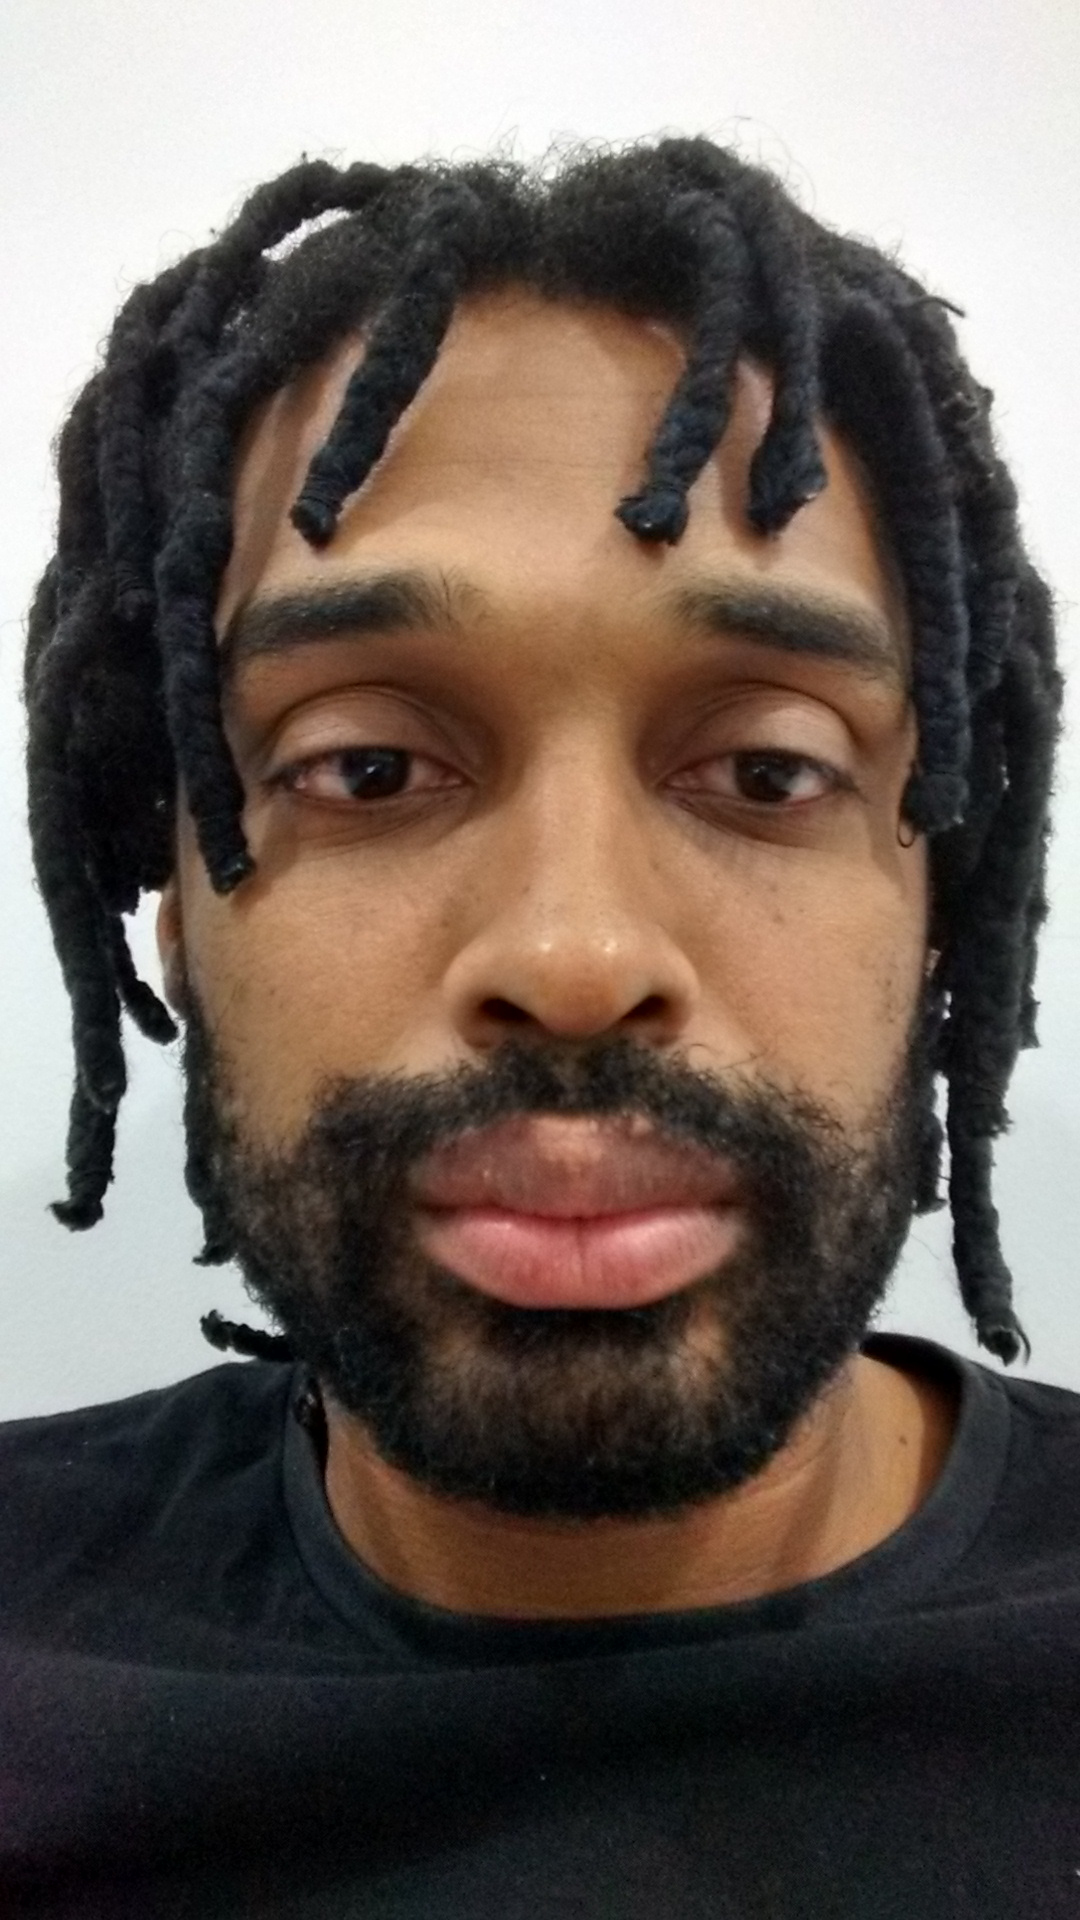
\includegraphics[width=1in,height=1.25in,clip,keepaspectratio]{Figure2.png}}]{Ericson Marquiere Reis Silva} received his B.Eng. degree in Control and Automation Engineering (2006) from the Pontificia Universidade Católica de Minas Gerais (PUC Minas), Belo Horizonte, Brazil, and his M.Sc. degree in Electrical and Electronics Engineering (2011) from the University of cyanwich, London, United Kingdom. He is currently pursuing his Ph.D. degree in Computer Science with PUC Minas and is a visiting student at the University of California, Irvine, USA. His research interest includes autonomous vehicles, embedded systems, machine learning, computer architecture, and parallel programming techniques.
\end{IEEEbiography}

\begin{IEEEbiography}
[{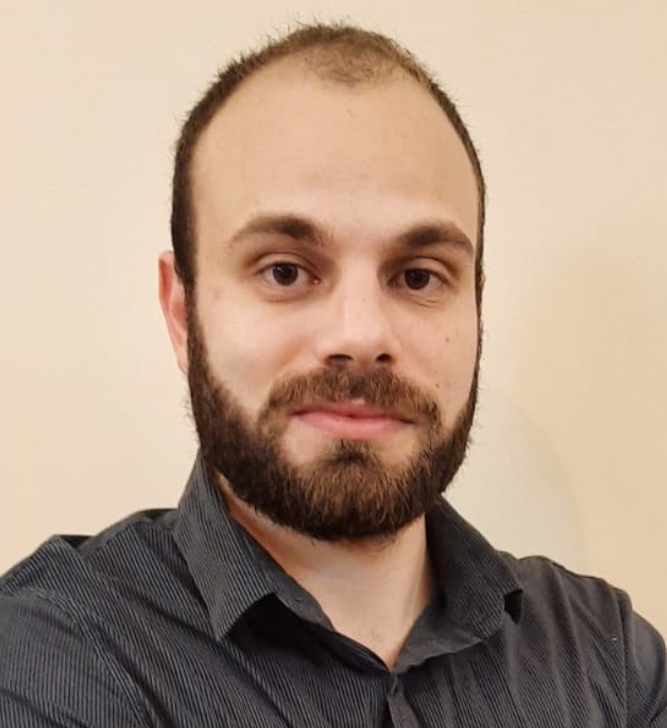
\includegraphics[width=1in,height=1.25in,clip,keepaspectratio]{Figure5.png}}]{Felipe Augusto Lara Soares} is a Ph.D. student in Informatics at the Pontifícia Universidade Católica de Minas Gerais (PUC Minas), Belo Horizonte, Brazil. He received his Master's in Informatics (2020) and Computer Engineering (2016) from PUC Minas. He is an Assistant Professor at PUC Minas, and his research interests are data analytics, machine learning, high-performance computing, autonomous vehicles, robotics, and internet-of-things.
\end{IEEEbiography}

\begin{IEEEbiography}[{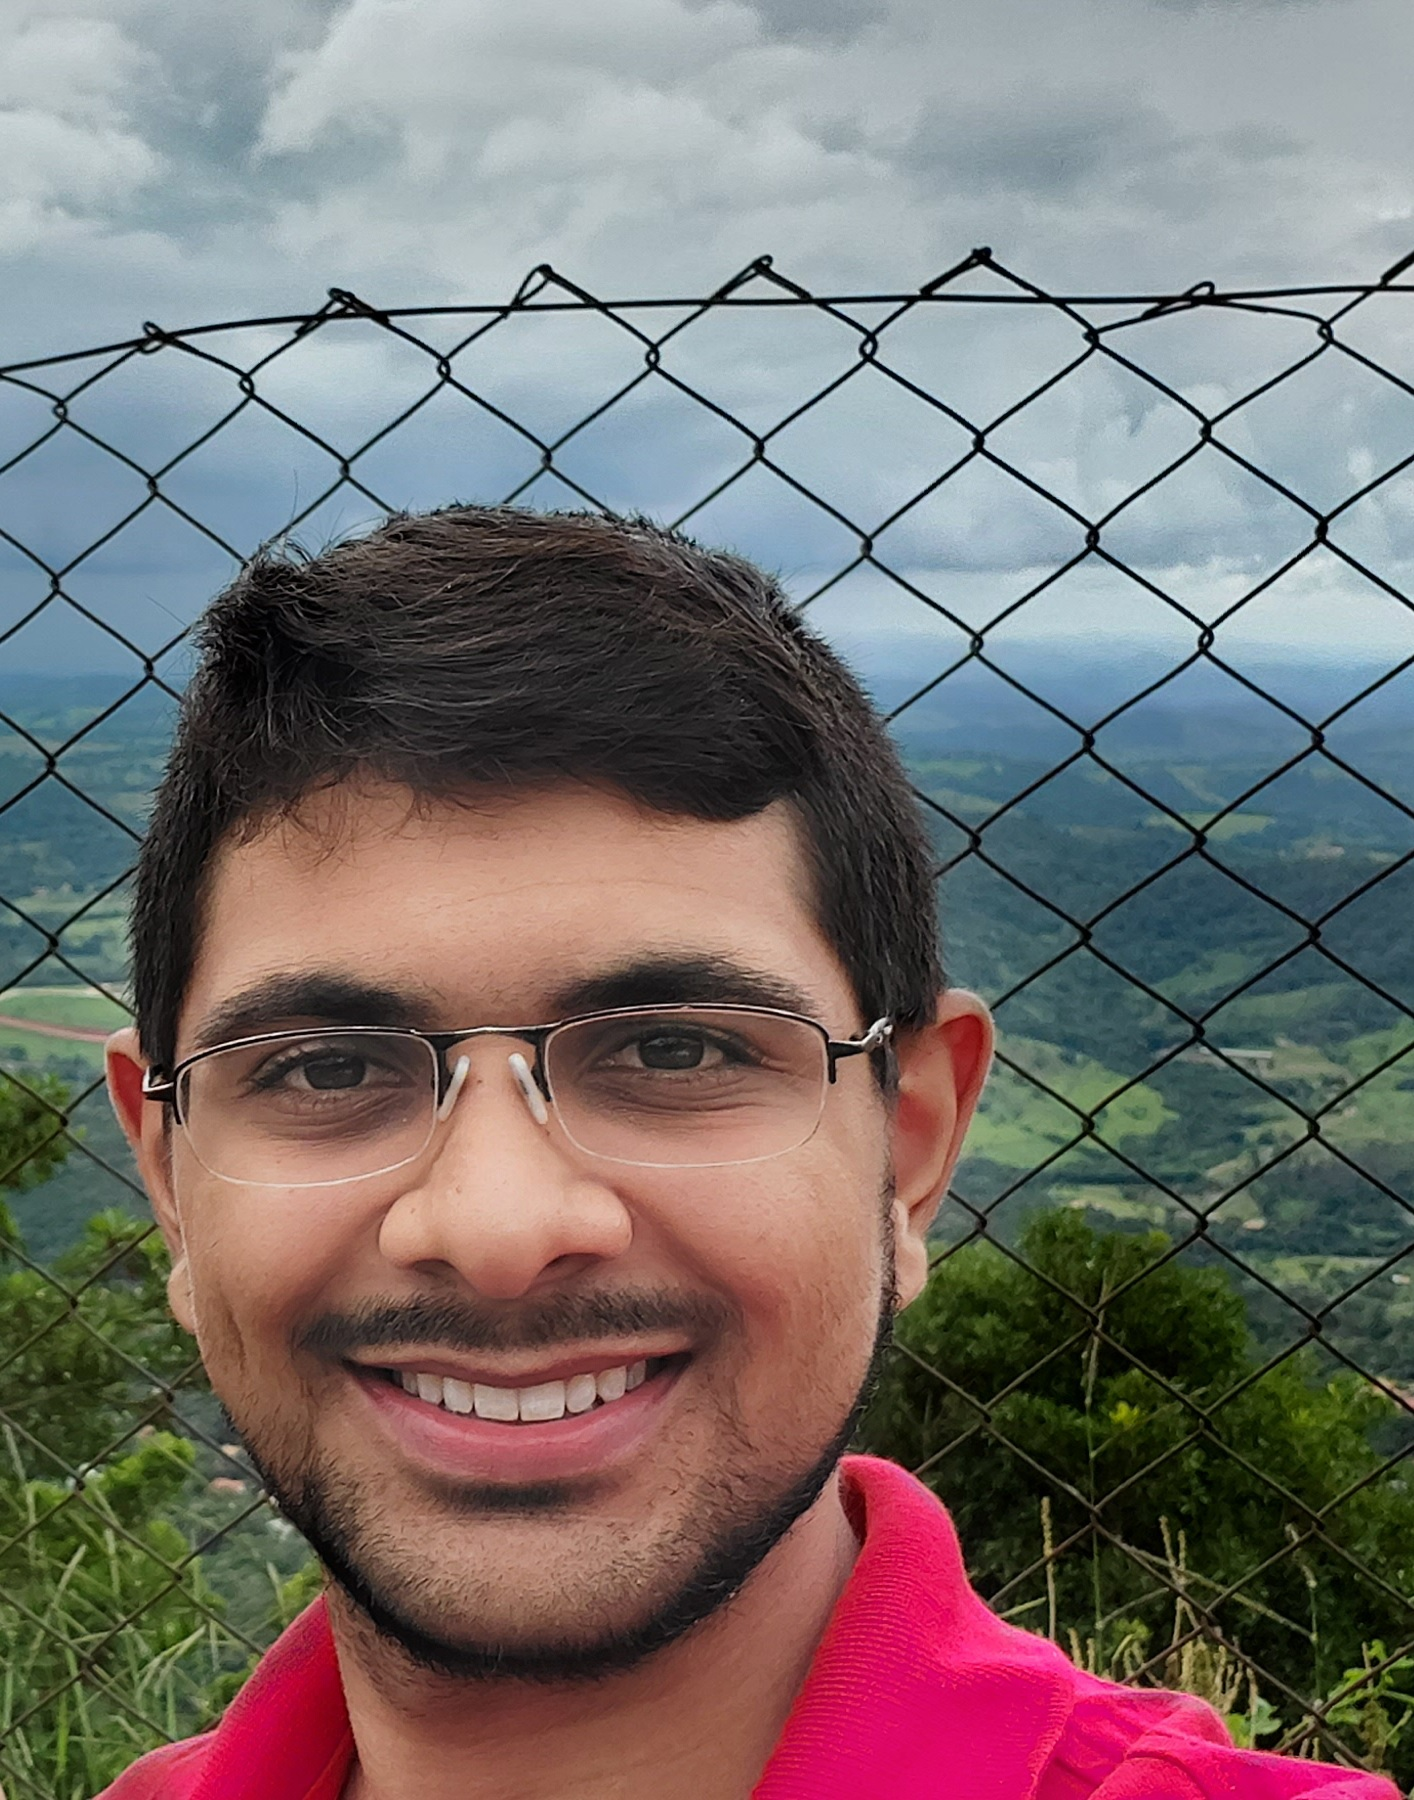
\includegraphics[width=1in,height=1.25in,clip,keepaspectratio]{Figure3.png}}]{Wenderson Júnio de Souza} received his B.Eng. degree in Computer Engineering (2021) from the Pontificia Universidade Católica de Minas Gerais (PUC Minas), Belo Horizonte, Brazil.  His research interest includes autonomous vehicles, high-performance computing, embedded systems, and machine learning.
\end{IEEEbiography}

% \vskip 0pt plus -1fil

\begin{IEEEbiography}[{
\includegraphics[width=1in,height=1.25in,clip,keepaspectratio]{Figure4.png}}]{Henrique Cota de Freitas} received his B.Sc. degree in Computer Science (2000) and M.Sc. degree in Electrical Engineering (2003) from the Pontifícia Universidade Católica de Minas Gerais (PUC Minas), Belo Horizonte, Brazil, and a Ph.D. in Computer Science (2009) from the Universidade Federal do Rio Grande do Sul (UFRGS). He was a visiting researcher at Université Grenoble Alpes, France, from 2015 to 2016. Henrique is an Associate Professor with the Department of Computer Science at PUC Minas. His research interest includes computer architecture, high-performance computing, heterogeneous computing, parallel computing, and autonomous vehicles.


\end{IEEEbiography}

% \IEEEPARstart{T}{his} file is intended to serve as a ``sample article file''
% for IEEE journal papers produced under \LaTeX\ using
% IEEEtran.cls version 1.8b and later. The most common elements are covered in the simplified and updated instructions in ``New\_IEEEtran\_how-to.pdf''. For less common elements you can refer back to the original ``IEEEtran\_HOWTO.pdf''. It is assumed that the reader has a basic working knowledge of \LaTeX. Those who are new to \LaTeX \ are encouraged to read Tobias Oetiker's ``The Not So Short Introduction to \LaTeX ,'' available at: \url{http://tug.ctan.org/info/lshort/english/lshort.pdf} which provides an overview of working with \LaTeX.

% \section{The Design, Intent, and \\ Limitations of the Templates}
% The templates are intended to {\bf{approximate the final look and page length of the articles/papers}}. {\bf{They are NOT intended to be the final produced work that is displayed in print or on IEEEXplore\textsuperscript{\textregistered}}}. They will help to give the authors an approximation of the number of pages that will be in the final version. The structure of the \LaTeX\ files, as designed, enable easy conversion to XML for the composition systems used by the IEEE. The XML files are used to produce the final print/IEEEXplore pdf and then converted to HTML for IEEEXplore.

% \section{Where to Get \LaTeX \ Help --- User Groups}
% The following online groups are helpful to beginning and experienced \LaTeX\ users. A search through their archives can provide many answers to common questions.
% \begin{list}{}{}
% \item{\url{http://www.latex-community.org/}} 
% \item{\url{https://tex.stackexchange.com/} }
% \end{list}

% \section{Other Resources}
% See \cite{ref1,ref2,ref3,ref4,ref5} for resources on formatting math into text and additional help in working with \LaTeX .

% \section{Text}
% For some of the remainer of this sample we will use dummy text to fill out paragraphs rather than use live text that may violate a copyright.

% Itam, que ipiti sum dem velit la sum et dionet quatibus apitet voloritet audam, qui aliciant voloreicid quaspe volorem ut maximusandit faccum conemporerum aut ellatur, nobis arcimus.
% Fugit odi ut pliquia incitium latum que cusapere perit molupta eaquaeria quod ut optatem poreiur? Quiaerr ovitior suntiant litio bearciur?

% Onseque sequaes rectur autate minullore nusae nestiberum, sum voluptatio. Et ratem sequiam quaspername nos rem repudandae volum consequis nos eium aut as molupta tectum ulparumquam ut maximillesti consequas quas inctia cum volectinusa porrum unt eius cusaest exeritatur? Nias es enist fugit pa vollum reium essusam nist et pa aceaqui quo elibusdandis deligendus que nullaci lloreri bla que sa coreriam explacc atiumquos simolorpore, non prehendunt lam que occum\cite{ref6} si aut aut maximus eliaeruntia dia sequiamenime natem sendae ipidemp orehend uciisi omnienetus most verum, ommolendi omnimus, est, veni aut ipsa volendelist mo conserum volores estisciis recessi nveles ut poressitatur sitiis ex endi diti volum dolupta aut aut odi as eatquo cullabo remquis toreptum et des accus dolende pores sequas dolores tinust quas expel moditae ne sum quiatis nis endipie nihilis etum fugiae audi dia quiasit quibus.
% \IEEEpubidadjcol
% Ibus el et quatemo luptatque doluptaest et pe volent rem ipidusa eribus utem venimolorae dera qui acea quam etur aceruptat.
% Gias anis doluptaspic tem et aliquis alique inctiuntiur?

% Sedigent, si aligend elibuscid ut et ium volo tem eictore pellore ritatus ut ut ullatus in con con pere nos ab ium di tem aliqui od magnit repta volectur suntio. Nam isquiante doluptis essit, ut eos suntionsecto debitiur sum ea ipitiis adipit, oditiore, a dolorerempos aut harum ius, atquat.

% Rum rem ditinti sciendunti volupiciendi sequiae nonsect oreniatur, volores sition ressimil inus solut ea volum harumqui to see\eqref{deqn_ex1a} mint aut quat eos explis ad quodi debis deliqui aspel earcius.

% \begin{equation}
% \label{deqn_ex1a}
% x = \sum_{i=0}^{n} 2{i} Q.
% \end{equation}

% Alis nime volorempera perferi sitio denim repudae pre ducilit atatet volecte ssimillorae dolore, ut pel ipsa nonsequiam in re nus maiost et que dolor sunt eturita tibusanis eatent a aut et dio blaudit reptibu scipitem liquia consequodi od unto ipsae. Et enitia vel et experferum quiat harum sa net faccae dolut voloria nem. Bus ut labo. Ita eum repraer rovitia samendit aut et volupta tecupti busant omni quiae porro que nossimodic temquis anto blacita conse nis am, que ereperum eumquam quaescil imenisci quae magnimos recus ilibeaque cum etum iliate prae parumquatemo blaceaquiam quundia dit apienditem rerit re eici quaes eos sinvers pelecabo. Namendignis as exerupit aut magnim ium illabor roratecte plic tem res apiscipsam et vernat untur a deliquaest que non cus eat ea dolupiducim fugiam volum hil ius dolo eaquis sitis aut landesto quo corerest et auditaquas ditae voloribus, qui optaspis exero cusa am, ut plibus.


% \section{Some Common Elements}
% \subsection{Sections and Subsections}
% Enumeration of section headings is desirable, but not required. When numbered, please be consistent throughout the article, that is, all headings and all levels of section headings in the article should be enumerated. Primary headings are designated with Roman numerals, secondary with capital letters, tertiary with Arabic numbers; and quaternary with lowercase letters. Reference and Acknowledgment headings are unlike all other section headings in text. They are never enumerated. They are simply primary headings without labels, regardless of whether the other headings in the article are enumerated. 

% \subsection{Citations to the Bibliography}
% The coding for the citations is made with the \LaTeX\ $\backslash${\tt{cite}} command. 
% This will display as: see \cite{ref1}.

% For multiple citations code as follows: {\tt{$\backslash$cite\{ref1,ref2,ref3\}}}
%  which will produce \cite{ref1,ref2,ref3}. For reference ranges that are not consecutive code as {\tt{$\backslash$cite\{ref1,ref2,ref3,ref9\}}} which will produce  \cite{ref1,ref2,ref3,ref9}

% \subsection{Lists}
% In this section, we will consider three types of lists: simple unnumbered, numbered, and bulleted. There have been many options added to IEEEtran to enhance the creation of lists. If your lists are more complex than those shown below, please refer to the original ``IEEEtran\_HOWTO.pdf'' for additional options.\\

% \subsubsection*{\bf A plain  unnumbered list}
% \begin{list}{}{}
% \item{bare\_jrnl.tex}
% \item{bare\_conf.tex}
% \item{bare\_jrnl\_compsoc.tex}
% \item{bare\_conf\_compsoc.tex}
% \item{bare\_jrnl\_comsoc.tex}
% \end{list}

% \subsubsection*{\bf A simple numbered list}
% \begin{enumerate}
% \item{bare\_jrnl.tex}
% \item{bare\_conf.tex}
% \item{bare\_jrnl\_compsoc.tex}
% \item{bare\_conf\_compsoc.tex}
% \item{bare\_jrnl\_comsoc.tex}
% \end{enumerate}

% \subsubsection*{\bf A simple bulleted list}
% \begin{itemize}
% \item{bare\_jrnl.tex}
% \item{bare\_conf.tex}
% \item{bare\_jrnl\_compsoc.tex}
% \item{bare\_conf\_compsoc.tex}
% \item{bare\_jrnl\_comsoc.tex}
% \end{itemize}





% \subsection{Figures}
% Fig. 1 is an example of a floating figure using the graphicx package.
%  Note that $\backslash${\tt{label}} must occur AFTER (or within) $\backslash${\tt{caption}}.
%  For figures, $\backslash${\tt{caption}} should occur after the $\backslash${\tt{includegraphics}}.

% \begin{figure}[!t]
% \centering
% 
\includegraphics[width=2.5in]{fig1}
% \caption{Simulation results for the network.}
% \label{fig_1}
% \end{figure}

% Fig. 2(a) and 2(b) is an example of a double column floating figure using two subfigures.
%  (The subfig.sty package must be loaded for this to work.)
%  The subfigure $\backslash${\tt{label}} commands are set within each subfloat command,
%  and the $\backslash${\tt{label}} for the overall figure must come after $\backslash${\tt{caption}}.
%  $\backslash${\tt{hfil}} is used as a separator to get equal spacing.
%  The combined width of all the parts of the figure should do not exceed the text width or a line break will occur.
% %
% \begin{figure*}[!t]
% \centering
% \subfloat[]{
\includegraphics[width=2.5in]{fig1}%
% \label{fig_first_case}}
% \hfil
% \subfloat[]{
\includegraphics[width=2.5in]{fig1}%
% \label{fig_second_case}}
% \caption{Dae. Ad quatur autat ut porepel itemoles dolor autem fuga. Bus quia con nessunti as remo di quatus non perum que nimus. (a) Case I. (b) Case II.}
% \label{fig_sim}
% \end{figure*}

% Note that often IEEE papers with multi-part figures do not place the labels within the image itself (using the optional argument to $\backslash${\tt{subfloat}}[]), but instead will
%  reference/describe all of them (a), (b), etc., within the main caption.
%  Be aware that for subfig.sty to generate the (a), (b), etc., subfigure
%  labels, the optional argument to $\backslash${\tt{subfloat}} must be present. If a
%  subcaption is not desired, leave its contents blank,
%  e.g.,$\backslash${\tt{subfloat}}[].


 

% \section{Tables}
% Note that, for IEEE-style tables, the
%  $\backslash${\tt{caption}} command should come BEFORE the table. Table captions use title case. Articles (a, an, the), coordinating conjunctions (and, but, for, or, nor), and most short prepositions are lowercase unless they are the first or last word. Table text will default to $\backslash${\tt{footnotesize}} as
%  the IEEE normally uses this smaller font for tables.
%  The $\backslash${\tt{label}} must come after $\backslash${\tt{caption}} as always.
 
% \begin{table}[!t]
% \caption{An Example of a Table\label{tab:table1}}
% \centering
% \begin{tabular}{|c||c|}
% \hline
% One & Two\\
% \hline
% Three & Four\\
% \hline
% \end{tabular}
% \end{table}

% \section{Algorithms}
% Algorithms should be numbered and include a short title. They are set off from the text with rules above and below the title and after the last line.

% \begin{algorithm}[H]
% \caption{Weighted Tanimoto ELM.}\label{alg:alg1}
% \begin{algorithmic}
% \STATE 
% \STATE {\textsc{TRAIN}}$(\mathbf{X} \mathbf{T})$
% \STATE \hspace{0.5cm}$ \textbf{select randomly } W \subset \mathbf{X}  $
% \STATE \hspace{0.5cm}$ N_\mathbf{t} \gets | \{ i : \mathbf{t}_i = \mathbf{t} \} | $ \textbf{ for } $ \mathbf{t}= -1,+1 $
% \STATE \hspace{0.5cm}$ B_i \gets \sqrt{ \textsc{max}(N_{-1},N_{+1}) / N_{\mathbf{t}_i} } $ \textbf{ for } $ i = 1,...,N $
% \STATE \hspace{0.5cm}$ \hat{\mathbf{H}} \gets  B \cdot (\mathbf{X}^T\textbf{W})/( \mathbb{1}\mathbf{X} + \mathbb{1}\textbf{W} - \mathbf{X}^T\textbf{W} ) $
% \STATE \hspace{0.5cm}$ \beta \gets \left ( I/C + \hat{\mathbf{H}}^T\hat{\mathbf{H}} \right )^{-1}(\hat{\mathbf{H}}^T B\cdot \mathbf{T})  $
% \STATE \hspace{0.5cm}\textbf{return}  $\textbf{W},  \beta $
% \STATE 
% \STATE {\textsc{PREDICT}}$(\mathbf{X} )$
% \STATE \hspace{0.5cm}$ \mathbf{H} \gets  (\mathbf{X}^T\textbf{W} )/( \mathbb{1}\mathbf{X}  + \mathbb{1}\textbf{W}- \mathbf{X}^T\textbf{W}  ) $
% \STATE \hspace{0.5cm}\textbf{return}  $\textsc{sign}( \mathbf{H} \beta )$
% \end{algorithmic}
% \label{alg1}
% \end{algorithm}

% Que sunt eum lam eos si dic to estist, culluptium quid qui nestrum nobis reiumquiatur minimus minctem. Ro moluptat fuga. Itatquiam ut laborpo rersped exceres vollandi repudaerem. Ulparci sunt, qui doluptaquis sumquia ndestiu sapient iorepella sunti veribus. Ro moluptat fuga. Itatquiam ut laborpo rersped exceres vollandi repudaerem. 
% \section{Mathematical Typography \\ and Why It Matters}

% Typographical conventions for mathematical formulas have been developed to {\bf provide uniformity and clarity of presentation across mathematical texts}. This enables the readers of those texts to both understand the author's ideas and to grasp new concepts quickly. While software such as \LaTeX \ and MathType\textsuperscript{\textregistered} can produce aesthetically pleasing math when used properly, it is also very easy to misuse the software, potentially resulting in incorrect math display.

% IEEE aims to provide authors with the proper guidance on mathematical typesetting style and assist them in writing the best possible article. As such, IEEE has assembled a set of examples of good and bad mathematical typesetting \cite{ref1,ref2,ref3,ref4,ref5}. 

% Further examples can be found at \url{http://journals.ieeeauthorcenter.ieee.org/wp-content/uploads/sites/7/IEEE-Math-Typesetting-Guide-for-LaTeX-Users.pdf}

% \subsection{Display Equations}
% The simple display equation example shown below uses the ``equation'' environment. To number the equations, use the $\backslash${\tt{label}} macro to create an identifier for the equation. LaTeX will automatically number the equation for you.
% \begin{equation}
% \label{deqn_ex1}
% x = \sum_{i=0}^{n} 2{i} Q.
% \end{equation}

% \noindent is coded as follows:
% \begin{verbatim}
% \begin{equation}
% \label{deqn_ex1}
% x = \sum_{i=0}^{n} 2{i} Q.
% \end{equation}
% \end{verbatim}

% To reference this equation in the text use the $\backslash${\tt{ref}} macro. 
% Please see (\ref{deqn_ex1})\\
% \noindent is coded as follows:
% \begin{verbatim}
% Please see (\ref{deqn_ex1})\end{verbatim}

% \subsection{Equation Numbering}
% {\bf{Consecutive Numbering:}} Equations within an article are numbered consecutively from the beginning of the
% article to the end, i.e., (1), (2), (3), (4), (5), etc. Do not use roman numerals or section numbers for equation numbering.

% \noindent {\bf{Appendix Equations:}} The continuation of consecutively numbered equations is best in the Appendix, but numbering
%  as (A1), (A2), etc., is permissible.\\

% \noindent {\bf{Hyphens and Periods}}: Hyphens and periods should not be used in equation numbers, i.e., use (1a) rather than
% (1-a) and (2a) rather than (2.a) for subequations. This should be consistent throughout the article.

% \subsection{Multi-Line Equations and Alignment}
% Here we show several examples of multi-line equations and proper alignments.

% \noindent {\bf{A single equation that must break over multiple lines due to length with no specific alignment.}}
% \begin{multline}
% \text{The first line of this example}\\
% \text{The second line of this example}\\
% \text{The third line of this example}
% \end{multline}

% \noindent is coded as:
% \begin{verbatim}
% \begin{multline}
% \text{The first line of this example}\\
% \text{The second line of this example}\\
% \text{The third line of this example}
% \end{multline}
% \end{verbatim}

% \noindent {\bf{A single equation with multiple lines aligned at the = signs}}
% \begin{align}
% a &= c+d \\
% b &= e+f
% \end{align}
% \noindent is coded as:
% \begin{verbatim}
% \begin{align}
% a &= c+d \\
% b &= e+f
% \end{align}
% \end{verbatim}

% The {\tt{align}} environment can align on multiple  points as shown in the following example:
% \begin{align}
% x &= y & X & =Y & a &=bc\\
% x' &= y' & X' &=Y' &a' &=bz
% \end{align}
% \noindent is coded as:
% \begin{verbatim}
% \begin{align}
% x &= y & X & =Y & a &=bc\\
% x' &= y' & X' &=Y' &a' &=bz
% \end{align}
% \end{verbatim}





% \subsection{Subnumbering}
% The amsmath package provides a {\tt{subequations}} environment to facilitate subnumbering. An example:

% \begin{subequations}\label{eq:2}
% \begin{align}
% f&=g \label{eq:2A}\\
% f' &=g' \label{eq:2B}\\
% \mathcal{L}f &= \mathcal{L}g \label{eq:2c}
% \end{align}
% \end{subequations}

% \noindent is coded as:
% \begin{verbatim}
% \begin{subequations}\label{eq:2}
% \begin{align}
% f&=g \label{eq:2A}\\
% f' &=g' \label{eq:2B}\\
% \mathcal{L}f &= \mathcal{L}g \label{eq:2c}
% \end{align}
% \end{subequations}

% \end{verbatim}

% \subsection{Matrices}
% There are several useful matrix environments that can save you some keystrokes. See the example coding below and the output.

% \noindent {\bf{A simple matrix:}}
% \begin{equation}
% \begin{matrix}  0 &  1 \\ 
% 1 &  0 \end{matrix}
% \end{equation}
% is coded as:
% \begin{verbatim}
% \begin{equation}
% \begin{matrix}  0 &  1 \\ 
% 1 &  0 \end{matrix}
% \end{equation}
% \end{verbatim}

% \noindent {\bf{A matrix with parenthesis}}
% \begin{equation}
% \begin{pmatrix} 0 & -i \\
%  i &  0 \end{pmatrix}
% \end{equation}
% is coded as:
% \begin{verbatim}
% \begin{equation}
% \begin{pmatrix} 0 & -i \\
%  i &  0 \end{pmatrix}
% \end{equation}
% \end{verbatim}

% \noindent {\bf{A matrix with square brackets}}
% \begin{equation}
% \begin{bmatrix} 0 & -1 \\ 
% 1 &  0 \end{bmatrix}
% \end{equation}
% is coded as:
% \begin{verbatim}
% \begin{equation}
% \begin{bmatrix} 0 & -1 \\ 
% 1 &  0 \end{bmatrix}
% \end{equation}
% \end{verbatim}

% \noindent {\bf{A matrix with curly braces}}
% \begin{equation}
% \begin{Bmatrix} 1 &  0 \\ 
% 0 & -1 \end{Bmatrix}
% \end{equation}
% is coded as:
% \begin{verbatim}
% \begin{equation}
% \begin{Bmatrix} 1 &  0 \\ 
% 0 & -1 \end{Bmatrix}
% \end{equation}\end{verbatim}

% \noindent {\bf{A matrix with single verticals}}
% \begin{equation}
% \begin{vmatrix} a &  b \\ 
% c &  d \end{vmatrix}
% \end{equation}
% is coded as:
% \begin{verbatim}
% \begin{equation}
% \begin{vmatrix} a &  b \\ 
% c &  d \end{vmatrix}
% \end{equation}\end{verbatim}

% \noindent {\bf{A matrix with double verticals}}
% \begin{equation}
% \begin{Vmatrix} i &  0 \\ 
% 0 & -i \end{Vmatrix}
% \end{equation}
% is coded as:
% \begin{verbatim}
% \begin{equation}
% \begin{Vmatrix} i &  0 \\ 
% 0 & -i \end{Vmatrix}
% \end{equation}\end{verbatim}

% \subsection{Arrays}
% The {\tt{array}} environment allows you some options for matrix-like equations. You will have to manually key the fences, but there are other options for alignment of the columns and for setting horizontal and vertical rules. The argument to {\tt{array}} controls alignment and placement of vertical rules.

% A simple array
% \begin{equation}
% \left(
% \begin{array}{cccc}
% a+b+c & uv & x-y & 27\\
% a+b & u+v & z & 134
% \end{array}\right)
% \end{equation}
% is coded as:
% \begin{verbatim}
% \begin{equation}
% \left(
% \begin{array}{cccc}
% a+b+c & uv & x-y & 27\\
% a+b & u+v & z & 134
% \end{array} \right)
% \end{equation}
% \end{verbatim}

% A slight variation on this to better align the numbers in the last column
% \begin{equation}
% \left(
% \begin{array}{cccr}
% a+b+c & uv & x-y & 27\\
% a+b & u+v & z & 134
% \end{array}\right)
% \end{equation}
% is coded as:
% \begin{verbatim}
% \begin{equation}
% \left(
% \begin{array}{cccr}
% a+b+c & uv & x-y & 27\\
% a+b & u+v & z & 134
% \end{array} \right)
% \end{equation}
% \end{verbatim}

% An array with vertical and horizontal rules
% \begin{equation}
% \left( \begin{array}{c|c|c|r}
% a+b+c & uv & x-y & 27\\ \hline
% a+b & u+v & z & 134
% \end{array}\right)
% \end{equation}
% is coded as:
% \begin{verbatim}
% \begin{equation}
% \left(
% \begin{array}{c|c|c|r}
% a+b+c & uv & x-y & 27\\
% a+b & u+v & z & 134
% \end{array} \right)
% \end{equation}
% \end{verbatim}
% Note the argument now has the pipe "$\vert$" included to indicate the placement of the vertical rules.


% \subsection{Cases Structures}
% Many times cases can be miscoded using the wrong environment, i.e., {\tt{array}}. Using the {\tt{cases}} environment will save keystrokes (from not having to type the $\backslash${\tt{left}}$\backslash${\tt{lbrace}}) and automatically provide the correct column alignment.
% \begin{equation*}
% {z_m(t)} = \begin{cases}
% 1,&{\text{if}}\ {\beta }_m(t) \\ 
% {0,}&{\text{otherwise.}} 
% \end{cases}
% \end{equation*}
% \noindent is coded as follows:
% \begin{verbatim}
% \begin{equation*}
% {z_m(t)} = 
% \begin{cases}
% 1,&{\text{if}}\ {\beta }_m(t),\\ 
% {0,}&{\text{otherwise.}} 
% \end{cases}
% \end{equation*}
% \end{verbatim}
% \noindent Note that the ``\&'' is used to mark the tabular alignment. This is important to get  proper column alignment. Do not use $\backslash${\tt{quad}} or other fixed spaces to try and align the columns. Also, note the use of the $\backslash${\tt{text}} macro for text elements such as ``if'' and ``otherwise.''

% \subsection{Function Formatting in Equations}
% Often, there is an easy way to properly format most common functions. Use of the $\backslash$ in front of the function name will in most cases, provide the correct formatting. When this does not work, the following example provides a solution using the $\backslash${\tt{text}} macro:

% \begin{equation*} 
%   d_{R}^{KM} = \underset {d_{l}^{KM}} {\text{arg min}} \{ d_{1}^{KM},\ldots,d_{6}^{KM}\}.
% \end{equation*}

% \noindent is coded as follows:
% \begin{verbatim}
% \begin{equation*} 
%  d_{R}^{KM} = \underset {d_{l}^{KM}} 
%  {\text{arg min}} \{ d_{1}^{KM},
%  \ldots,d_{6}^{KM}\}.
% \end{equation*}
% \end{verbatim}

% \subsection{ Text Acronyms Inside Equations}
% This example shows where the acronym ``MSE" is coded using $\backslash${\tt{text\{\}}} to match how it appears in the text.

% \begin{equation*}
%  \text{MSE} = \frac {1}{n}\sum _{i=1}^{n}(Y_{i} - \hat {Y_{i}})^{2}
% \end{equation*}

% \begin{verbatim}
% \begin{equation*}
%  \text{MSE} = \frac {1}{n}\sum _{i=1}^{n}
% (Y_{i} - \hat {Y_{i}})^{2}
% \end{equation*}
% \end{verbatim}

% \section{Conclusion}
% The conclusion goes here.


% \section*{Acknowledgments}
% This should be a simple paragraph before the References to thank those individuals and institutions who have supported your work on this article.



% {\appendix[Proof of the Zonklar Equations]
% Use $\backslash${\tt{appendix}} if you have a single appendix:
% Do not use $\backslash${\tt{section}} anymore after $\backslash${\tt{appendix}}, only $\backslash${\tt{section*}}.
% If you have multiple appendixes use $\backslash${\tt{appendices}} then use $\backslash${\tt{section}} to start each appendix.
% You must declare a $\backslash${\tt{section}} before using any $\backslash${\tt{subsection}} or using $\backslash${\tt{label}} ($\backslash${\tt{appendices}} by itself
%  starts a section numbered zero.)}



% %{\appendices
% %\section*{Proof of the First Zonklar Equation}
% %Appendix one text goes here.
% % You can choose not to have a title for an appendix if you want by leaving the argument blank
% %\section*{Proof of the Second Zonklar Equation}
% %Appendix two text goes here.}



% \section{References Section}
% You can use a bibliography generated by BibTeX as a .bbl file.
%  BibTeX documentation can be easily obtained at:
%  http://mirror.ctan.org/biblio/bibtex/contrib/doc/
%  The IEEEtran BibTeX style support page is:
%  http://www.michaelshell.org/tex/ieeetran/bibtex/
 
%  % argument is your BibTeX string definitions and bibliography database(s)
% %\bibliography{IEEEabrv,../bib/paper}
% %
% \section{Simple References}
% You can manually copy in the resultant .bbl file and set second argument of $\backslash${\tt{begin}} to the number of references
%  (used to reserve space for the reference number labels box).

% \begin{thebibliography}{1}
% \bibliographystyle{IEEEtran}

% \bibitem{ref1}
% {\it{Mathematics Into Type}}. American Mathematical Society. [Online]. Available: https://www.ams.org/arc/styleguide/mit-2.pdf

% \bibitem{ref2}
% T. W. Chaundy, P. R. Barrett and C. Batey, {\it{The Printing of Mathematics}}. London, U.K., Oxford Univ. Press, 1954.

% \bibitem{ref3}
% F. Mittelbach and M. Goossens, {\it{The \LaTeX Companion}}, 2nd ed. Boston, MA, USA: Pearson, 2004.

% \bibitem{ref4}
% G. Gr\"atzer, {\it{More Math Into LaTeX}}, New York, NY, USA: Springer, 2007.

% \bibitem{ref5}M. Letourneau and J. W. Sharp, {\it{AMS-StyleGuide-online.pdf,}} American Mathematical Society, Providence, RI, USA, [Online]. Available: http://www.ams.org/arc/styleguide/index.html

% \bibitem{ref6}
% H. Sira-Ramirez, ``On the sliding mode control of nonlinear systems,'' \textit{Syst. Control Lett.}, vol. 19, pp. 303--312, 1992.

% \bibitem{ref7}
% A. Levant, ``Exact differentiation of signals with unbounded higher derivatives,''  in \textit{Proc. 45th IEEE Conf. Decis.
% Control}, San Diego, CA, USA, 2006, pp. 5585--5590. DOI: 10.1109/CDC.2006.377165.

% \bibitem{ref8}
% M. Fliess, C. Join, and H. Sira-Ramirez, ``Non-linear estimation is easy,'' \textit{Int. J. Model., Ident. Control}, vol. 4, no. 1, pp. 12--27, 2008.

% \bibitem{ref9}
% R. Ortega, A. Astolfi, G. Bastin, and H. Rodriguez, ``Stabilization of food-chain systems using a port-controlled Hamiltonian description,'' in \textit{Proc. Amer. Control Conf.}, Chicago, IL, USA,
% 2000, pp. 2245--2249.

% \end{thebibliography}


% \newpage

% \section{Biography Section}
% If you have an EPS/PDF photo (graphicx package needed), extra braces are
%  needed around the contents of the optional argument to biography to prevent
%  the LaTeX parser from getting confused when it sees the complicated
%  $\backslash${\tt{includegraphics}} command within an optional argument. (You can create
%  your own custom macro containing the $\backslash${\tt{includegraphics}} command to make things
%  simpler here.)
 
% \vspace{11pt}

% \bf{If you include a photo:}\vspace{-33pt}
% \begin{IEEEbiography}[{
\includegraphics[width=1in,height=1.25in,clip,keepaspectratio]{fig1}}]{Michael Shell}
% Use $\backslash${\tt{begin\{IEEEbiography\}}} and then for the 1st argument use $\backslash${\tt{includegraphics}} to declare and link the author photo.
% Use the author name as the 3rd argument followed by the biography text.
% \end{IEEEbiography}

% \vspace{11pt}

% \bf{If you will not include a photo:}\vspace{-33pt}
% \begin{IEEEbiographynophoto}{John Doe}
% Use $\backslash${\tt{begin\{IEEEbiographynophoto\}}} and the author name as the argument followed by the biography text.
% \end{IEEEbiographynophoto}




\vfill

\end{document}


